\documentclass[12pt]{report}
\usepackage[greek]{babel}
\usepackage{fontspec}
\usepackage{graphicx}
\usepackage{booktabs}
%!TEX TS-program = xelatex
%!TEX encoding = UTF-8 Unicode
\usepackage{xltxtra}
\usepackage{titlesec}
\setmainfont{Times New Roman}
\usepackage{subcaption}
\usepackage[export]{adjustbox}
\usepackage{wrapfig}
\usepackage[locale=DE]{siunitx}
\usepackage[a4paper, 
    top=3cm, 
    bottom=2.54cm, 
    left=2.54cm, 
    right=2.54cm,
    headheight=28pt,  % Critical for header space
    headsep=1.2cm,
    includehead,      % Include header in page area
    includefoot]{geometry}
\usepackage{hyperref}
\usepackage{makecell}
\usepackage{float}
\usepackage{chngcntr}
\usepackage{caption}
\usepackage[justification=centering]{caption}
\usepackage[noabbrev]{cleveref}

\usepackage[font={smaller,it}]{caption}
\usepackage[backend=biber, style=apa, sorting=ynt]{biblatex}
\usepackage{setspace}
\usepackage{tablefootnote}
\usepackage{csquotes}
\usepackage{longtable}
\usepackage{array}
\usepackage{fancyhdr}
\usepackage{etoolbox}
\usepackage{tocloft}
\usepackage{listings}
\usepackage{cleveref}
\usepackage{xcolor}
\addbibresource{references.bib}
\usepackage{nomencl}
\usepackage[table]{xcolor}
\usepackage{multirow}
\captionsetup{tablename=Πίνακας}
\renewcommand\theadfont{\bfseries}
\renewcommand{\arraystretch}{1.5}

% \pagestyle{fancy}
% \fancyhf{} % Clear all headers/footers
% \addto\captionsgreek{%
%   \crefname{lstlisting}{κώδικας}{κώδικες}%
%   \Crefname{lstlisting}{Κώδικας}{Κώδικες}%
%   \crefname{appendix}{παράρτημα}{παραρτήματα}%
%   \Crefname{appendix}{Παράρτημα}{Παραρτήματα}%
% }

\captionsetup[figure]{
  labelformat=simple,
  labelsep=space,
  name=Εικόνα,
  format=plain
}
\counterwithin{figure}{chapter}

\captionsetup[table]{
  labelformat=simple,
  labelsep=space,
  name=Πίνακας,
  format=plain
}
\counterwithin{table}{chapter}

\renewcommand{\thesubfigure}{\roman{subfigure}}
\renewcommand{\thesubtable}{\roman{subtable}}

\titleformat{\chapter}[display]
    {\fontsize{16pt}{18pt}\selectfont\bfseries\raggedright}
    {\appendixname\ \thechapter}
    {0pt}
    {}
\titlespacing*{\chapter}{0pt}{0pt}{18pt}

\lstset{
    basicstyle=\fontsize{9}{11}\selectfont\ttfamily, % Courier New equivalent
    breaklines=true,
    frame=single,
    numbers=left,
    numberstyle=\tiny,
    stepnumber=1,
    tabsize=4,
    backgroundcolor=\color{gray!5},
    keywordstyle=\color{blue},
    commentstyle=\color{green!50!black},
    stringstyle=\color{red},
    showstringspaces=false
}

\fancypagestyle{mainstyle}{
    \fancyhf{}
    \fancyhead[L]{\hspace{2em}
\includegraphics[height=1.21cm,width=3.24cm]{university1-logo.png}}
    \fancyhead[C]{\raisebox{1ex}{%
        \parbox{\dimexpr\textwidth-7.5cm-4em\relax}{%
            \itshape\footnotesize%
            Κωνσταντίνος Περπερίδης\\%
            Ανάλυση δεδομένων γονιδιακής έκφρασης\\%
            και χαρτογράφηση λειτουργικών δικτύων\\%
            στη νόσο του Πάρκινσον%
        }}}
    \fancyhead[R]{
\includegraphics[height=1.21cm,width=4cm]{university2-logo.png}\hspace{2em}}
    \fancyfoot[C]{\thepage}
    \renewcommand{\headrulewidth}{0pt}
    % Remove the headsep from here since we set it in geometry
}


\fancypagestyle{plain}{
    \fancyhf{}
    \fancyfoot[C]{\thepage}
    \renewcommand{\headrulewidth}{0pt}
}

\makeatletter

\let\oldchapter\chapter
\renewcommand{\chapter}{\@ifstar{\starchapter}{\nostarchapter}}
\newcommand{\starchapter}[1]{\oldchapter*{#1}\thispagestyle{mainstyle}}
\newcommand{\nostarchapter}[1]{\oldchapter{#1}\thispagestyle{mainstyle}}
\makeatother

\makenomenclature
\renewcommand{\nomname}{Συντομογραφίες και Ακρωνύμια} % Custom title
\renewcommand{\nomlabelwidth}{2.5cm} % Adjust as needed

% Formatting to match your document
\renewcommand{\nompreamble}{\vspace{6pt}} % Space before list
\setlength{\nomitemsep}{6pt} 

% Reduce spacing in TOC
\setlength{\cftbeforechapskip}{6pt} % Space before chapter entries (was ~10pt)
\setlength{\cftbeforesecskip}{3pt} % Space before section entries
\setlength{\cftbeforesubsecskip}{3pt} % Space before subsection entries

% Add dot leaders for chapters (normally missing in report class)
\renewcommand{\cftchapleader}{\cftdotfill{\cftdotsep}} % Dot leaders for chapters
\renewcommand{\cftsecleader}{\cftdotfill{\cftdotsep}} % Ensures section leaders
\renewcommand{\cftsubsecleader}{\cftdotfill{\cftdotsep}} % Subsection leaders

% Font settings for TOC entries
\renewcommand{\cftchapfont}{\normalfont} % Chapter font
\renewcommand{\cftchappagefont}{\normalfont} % Chapter page number font

\onehalfspacing % 1.5 line spacing

% Header settings
\newlength{\logoheight}
\setlength{\logoheight}{1.21cm}
\newlength{\logowidth}
\setlength{\logowidth}{3.24cm}
\newlength{\headertextwidth}
\setlength{\headertextwidth}{\dimexpr\textwidth-2\logowidth-2em\relax}

\newcommand{\frontmatter}{
    \cleardoublepage
    \pagenumbering{roman}
    \pagestyle{plain} % Simple page numbers only
    \setcounter{page}{1} % Explicit reset
}

% Chapter formatting
\titleformat{\chapter}[display]
    {\fontsize{16pt}{18pt}\selectfont\bfseries\raggedright}
    {\thechapter}
    {0pt}
    {}
\titlespacing*{\chapter}{0pt}{0pt}{18pt}

% Section formatting
\titleformat{\section}
    {\fontsize{14pt}{12pt}\selectfont\bfseries\raggedright}
    {\thesection}
    {1em}
    {}
\titlespacing*{\section}{0pt}{12pt}{12pt}

% Subsection formatting
\titleformat{\subsection}
    {\fontsize{12pt}{6pt}\selectfont\bfseries\raggedright}
    {\thesubsection}
    {1em}
    {}
\titlespacing*{\subsection}{0pt}{0pt}{6pt}

% Subsubsection formatting
\titleformat{\subsubsection}
    {\fontsize{12pt}{6pt}\selectfont\bfseries\itshape\raggedright}
    {}
    {0pt}
    {}
\titlespacing*{\subsubsection}{0pt}{0pt}{6pt}

% Paragraph settings
\setlength{\parindent}{0pt}
\setlength{\parskip}{6pt}

% Caption settings
\captionsetup{
    font=footnotesize,
    labelfont=bf,
    justification=centering,
    singlelinecheck=off,
    skip=6pt,
    belowskip=12pt
}

\captionsetup[subfigure]{
    font=footnotesize
}
\DeclareCaptionLabelFormat{chapter}{\thechapter.#1}
% \captionsetup[figure]{labelformat=chapter}
% \captionsetup[table]{labelformat=chapter}

% Prevent figure/table captions from breaking across pages
% \pretocmd{\figure}{\begin{minipage}{\linewidth}}{}{}
% \apptocmd{\endfigure}{\end{minipage}}{}{}
% \pretocmd{\table}{\begin{minipage}{\linewidth}}{}{}
% \apptocmd{\endtable}{\end{minipage}}{}{}

% Footnote settings
\renewcommand{\footnotesize}{\fontsize{10pt}{1}\selectfont}
\let\oldfootnote\footnote
\renewcommand{\footnote}[1]{\oldfootnote{\onehalfspacing #1}}


% \title{\fontsize{16pt}{18pt}\selectfont\bfseries Ανάλυση δεδομένων γονιδιακής έκφρασης και χαρτογράφηση λειτουργικών δικτύων στη νόσο του Πάρκινσον}
% \author{Κωνσταντίνος Περπερίδης}
% \date{\today}
% \maketitle

\makeatletter
\renewcommand{\@makechapterhead}[1]{%
  \vspace*{0pt}%
  {\parindent \z@ \raggedright \normalfont
    \fontsize{16pt}{18pt}\selectfont\bfseries
    \mbox{\thechapter.\ #1}\par
    \nobreak
    \vskip 18pt
  }}
\makeatother

\makeatletter
\newcommand{\addtotoc}[1]{
    \cleardoublepage
    \phantomsection
    \addcontentsline{toc}{chapter}{#1}
}
\renewcommand{\maketitle}{
    \begin{titlepage}
        % \null\vfill
        \noindent
        \begin{minipage}[t]{0.6\textwidth}
            \centering
            
\includegraphics[height=2.4cm,width=6cm]{university1-logo.png}\\
            \fontsize{12pt}{14pt}\selectfont
            Σχολή Θετικών Επιστημών και Τεχνολογίας
        \end{minipage}
        \hfill
        \begin{minipage}[t]{0.4\textwidth}
            \centering
            
\includegraphics[height=1.8cm,width=6.5cm]{university2-logo.png}\\
            \fontsize{12pt}{14pt}\selectfont
            Τμήμα Πληροφορικής
        \end{minipage}
        \vspace*{2cm}
        \begin{center}
            \fontsize{16pt}{14pt}\selectfont
            Διαπανεπιστημιακό Μεταπτυχιακό Πρόγραμμα Σπουδών\\[14pt]
            Βιοπληροφορική και Νευροπληροφορική\\[48pt]
            Μεταπτυχιακή Διπλωματική Εργασία\\[24pt]
    
            {\fontsize{16pt}{18pt}\selectfont\bfseries \@title\\[18pt]}
            {\large \@author\\[12pt]}\\[24pt]
            \fontsize{12pt}{14pt}\selectfont
            Επιβλέπων καθηγητής: Μάριος Κροκίδης\\
            \vspace{5cm}
            \fontsize{14pt}{16pt}\selectfont
            Κιλκίς, {\large \@date}
        \end{center}
        % \vfill\null
    \end{titlepage}
}
\makeatother

% Document body
\begin{document}
\frontmatter

\title{Ανάλυση δεδομένων γονιδιακής έκφρασης και χαρτογράφηση λειτουργικών δικτύων στη νόσο του Πάρκινσον}
\author{Κωνσταντίνος Περπερίδης}
\date{\today}
\maketitle
\thispagestyle{empty} 
\cleardoublepage
\thispagestyle{empty} 
\vspace*{\fill} % Push content to vertical center
\begin{center}
\fontsize{10pt}{12pt}\selectfont
\textcopyright
Η παρούσα εργασία αποτελεί πνευματική ιδιοκτησία του/της φοιτητή/φοιτήτριας («συγγραφέας/δημιουργός»)
που την εκπόνησε. Στο πλαίσιο της πολιτικής ανοικτής πρόσβασης ο συγγραφέας/δημιουργός εκχωρεί στο
ΕΑΠ, μη αποκλειστική άδεια χρήσης του δικαιώματος αναπαραγωγής, προσαρμογής, δημόσιου δανεισμού,
παρουσίασης στο κοινό και ψηφιακής διάχυσής τους διεθνώς, σε ηλεκτρονική μορφή και σε οποιοδήποτε
μέσο, για διδακτικούς και ερευνητικούς σκοπούς, άνευ ανταλλάγματος και για όλο το χρόνο διάρκειας των
δικαιωμάτων πνευματικής ιδιοκτησίας. Η ανοικτή πρόσβαση στο πλήρες κείμενο για μελέτη και ανάγνωση
δεν σημαίνει καθ’ οιονδήποτε τρόπο παραχώρηση δικαιωμάτων διανοητικής ιδιοκτησίας του
συγγραφέα/δημιουργού ούτε επιτρέπει την αναπαραγωγή, αναδημοσίευση, αντιγραφή, αποθήκευση, πώληση,
εμπορική χρήση, μετάδοση, διανομή, έκδοση, εκτέλεση, «μεταφόρτωση» (downloading), «ανάρτηση»
(uploading), μετάφραση, τροποποίηση με οποιονδήποτε τρόπο, τμηματικά ή περιληπτικά της εργασίας, χωρίς
τη ρητή προηγούμενη έγγραφη συναίνεση του συγγραφέα/δημιουργού. Ο συγγραφέας/δημιουργός διατηρεί
το σύνολο των ηθικών και περιουσιακών του δικαιωμάτων.
\end{center}
\vspace*{\fill} % Ensure it stays at bottom
\clearpage


\clearpage
\thispagestyle{empty} % No header/footer
\begin{center}
    
    \begin{minipage}[t]{0.45\textwidth}
        \centering
        
\includegraphics[height=2.4cm,width=6cm]{university1-logo.png}\\
    \end{minipage}
    \hfill
    \begin{minipage}[t]{0.45\textwidth}
        \centering
        
\includegraphics[height=1.8cm,width=6.5cm]{university2-logo.png}\\
    \end{minipage}
    \vspace*{2cm}
    
    \fontsize{18pt}{22pt}\selectfont\
        Ανάλυση δεδομένων γονιδιακής έκφρασης και χαρτογράφηση λειτουργικών δικτύων στη νόσο του Πάρκινσον\\
    \vspace*{2.5cm}
    \large Κωνσταντίνος Περπερίδης\\
    \vspace*{2.5cm}
    \begin{center}
    \fontsize{12pt}{14pt}\selectfont
    Επιτροπή Επίβλεψης Διπλωματικής Εργασίας\\[16pt]
    \begin{minipage}[t]{0.45\textwidth}
        \centering
        \fontsize{12pt}{14pt}\selectfont
        \textbf{Επιβλέπων Καθηγητή}\\
        Μάριος Κροκίδης\\
        Επίκουρος Καθηγητής - Ιόνιο Πανεπιστήμιο
    \end{minipage}
    \hfill % Maximizes horizontal space between minipages
    \begin{minipage}[t]{0.45\textwidth}
        \centering
        \fontsize{12pt}{14pt}\selectfont
        \textbf{Συν-Επιβλέπων Καθηγητής}\\
        Θεμιστοκλής Έξαρχος\\
        Αναπληρωτής Καθηγητής - Ιόνιο Πανεπιστήμιο
    \end{minipage}
    \end{center}
    \vspace*{2.5cm}
    \fontsize{14pt}{16pt}\selectfont
    Πάτρα, {\large \today}
    
    \vfill
\end{center}
\clearpage

\cleardoublepage
\pagestyle{mainstyle}

\chapter*{Περίληψη}
\addcontentsline{toc}{chapter}{Περίληψη}
    \par
        H εργασία αυτή διαπραγματεύεται την ανάλυση μεταγραφικών δεδομένων αλληλούχισης RNA από δείγματα ολικού αίματος, καθώς και την χαρτογράφηση πιθανών λειτουργικών δικτύων στη νόσο του Πάρκινσον. Σκοπό αποτελεί η εφαρμογή κατάλληλων βιοπληροφοριακών εργαλείων προκειμένου να εντοπιστούν διαφορές στη γονιδιακή έκφραση μεταξύ συγκεκριμένων δεδομένων της νόσου και παράλληλα να αναζητηθούν γονίδια-στόχοι που εμπλέκονται στην παθοφυσιολογία.
    \par
        Η νόσος του Πάρκινσον χαρακτηρίζεται από έντονη κινητική δυσχέρεια με χαρακτηριστικό τρόμο στα άκρα και οφείλεται στην απώλεια ντοπαμινεργικών νευρώνων στην μέλαινα ουσία του εγκεφάλου. Η απώλεια λειτουργικών νευρώνων οδηγεί στην μείωση έκλυσης του νευροδιαβιβαστή της Ντοπαμίνης και οφείλεται στην συσσώρευση της πρωτεΐνης α-Συνουκλεϊνης και τη διαμόρφοση των λεγόμενων σωμάτιων Lewy εντός του κυττοπλάσματος των ντοπαμινεργικών νευρώνων (\emph{\cite{Balestrino2020ParkinsonDisease}}).
    \par
        Τα δείγματα προέρχονται από μια εκτεταμένη μελέτη, την Parkinson Progression Markers Initiative \emph{(PPMI\footnote{https://www.ppmi-info.org/})} τα οποία διανέμονται διαδικτυακά κατόπιν εγγραφής στις σελίδας του Imaging and Data Archive \emph{(IDA\footnote{https://ida.loni.usc.edu/})}. Πρόκειται για μια πολυδιάστατη μελέτη, καθώς πέραν των δεδομένων αλληλούχισης μεταγραφώματος διανέμονται μεταξύ άλλων και δεδομένα πρωτεομικής, μεθυλίωσης, κλινικών μελετών και απεικονιστικών εξετάσεων από ομάδες νοσούντων, ελέγχου αλλά και ατόμων με πιθανή γενετική προδιάθεση, ως φορείς γενετικών μεταλλάξεων σε γνωστά γονίδια τα οποία εμπλέκονται στην παθοφυσιολογία της νόσου.
    \par
        Καθώς τα διαγνωστικά πρωτόκολλα στηρίζονται κατά βάση σε κλινική αξιολόγηση των κινητικών συμπτωμάτων από ειδικούς νευρολόγους. Έχουν καθιερωθεί πρωτόκολλα αξιολόγησης κλινικών συμπτωμάτων, τα οποία στηρίζουν τη διαφορική διάγνωση (\emph{\cite{Koller2018TableGuidelines}}), τα συμπτώματα που παρουσιάζουν κινητική παθολογία είναι πιθανόν να αλληλεπικαλύπτονται με άλλες παθήσεις του νευρικού συστήματος (\emph{\cite{Tolosa2021ChallengesDisease}}). 
    \par
        Μια έγκαιρη διάγνωση η οποία στηρίζεται σε βιοδείκτες, όπως ενδείξεις εγκεφαλογραφημάτων, απεικονιστικών εξετάσεων όπως αυτής της μαγνητικής τομογραφίας εγκεφάλου αλλά και βιολογικού υλικού όπως εγκεφαλονωτιαίου υγρού αλλά και προϊόντα αίματος δεν έχουν καθιερωθεί καθώς ποικίλες έρευνες διαπραγματεύονται την ανεύρεση βιοδεικτών από διάφορες πηγές του οργανισμού (\emph{\cite{Miller2015BiomarkersFuture}}) (\emph{\cite{Maitin2022SurveyReview}}).
    \par
        Στην παρούσα εργασία χρησιμοποιούνται δείγματα ολικού αίματος ως μια προσιτή και πλούσια πηγή βιολογικής πληροφορίας. Ταυτόχρονα η αφθονία μεταγραφικής πληροφορίας που εμπεριέχεται στο αίμα, καθιστά μια εξαιρετική πρόκληση στην εύρεση και διαφοροποίηση σημαντικής πληροφορίας ως προς την αναγνώριση πιθανών βιοδεικτών και λειτουργικών δικτύων που θα μπορούσαν να επιτρέψουν τον συσχετισμό με τη νόσο του Πάρκινσον. Άρα, το βιολογικό ερώτημα που επιχειρεί να προσεγγίσει η παρούσα εργασία είναι, αν υπάρχουν μεταγραφομικοί μάρτυρες στο αίμα που θα μπορούσαν να συνοδέψουν συντηρητικές ή καινοτόμες προσεγγίσεις και μεθόδους με στόχο της αξιόπιστης διάγνωσης της νόσου του Πάρκινσον.
    \par
        Τα εργαλεία της βιοπληροφορικής που χρησιμοποιήθηκαν σε αυτή τη διπλωματική εργασία είναι μέθοδοι στατιστικής ανάλυσης, όπως η διαφορική ανάλυση γονιδιακής έκφρασης, η ανάλυση εμπλουτισμού και η μηχανική μάθηση, για την ανεύρεση χαρακτηριστικών που καθιστούν πιθανή την αναγνώριση της νόσου αλλά και την διασταύρωση των αποτελεσμάτων με πληροφορίες από βάσεις δεδομένων σχολιασμού.
        
    \cleardoublepage

    \chapter*{Abstract}
    \addcontentsline{toc}{chapter}{Abstract}
        \selectlanguage{english}
            \par
                This thesis handles the analysis of transcriptome data from RNA sequencing on whole-blood samples and the mapping of functional gene networks in Parkinson's disease. It aims at the application of suitable bioinformatics toolsets in order to recognise differences in gene expressions between particular data of the disease and in parallel to search for target genes with possible involvement in the pathophysiology.
            \par
                Parkinson's disease on the surface is defined by intense movement distress with a characteristic tremor on the limbs which is assumed to be due to the loss of dopaminergic neurons in the substantia nigra of the brain. The loss of functional neurons leads to progressive reduction of the neurotransmitter Dopamine and effectively happens because of accumulation of α-Synuclein to Lewy bodies in the inside of the dopaminergic cells (\emph{\cite{Balestrino2020ParkinsonDisease}}).
            \par
                The samples used in the this thesis originate from a large-scale study, the Parkinson Progression Markers Initiative (\emph{PPMI}) which are made available to download on the internet after registration on the pages of the Imaging and Data Archive (\emph{IDA}). It is indeed a multi-dimensional study since there are results from several examinations available apart from genetic data, such as Proteomics results, Methylation profiles, Clinical studies and Imaging results from case and control cohorts and dditionally from individuals with a possible genetic predisposition as carriers of genetic mutations in genes that are known to be involved in the pathophysiology of the disease.
            \par
                Since the diagnostic protocols are based on clinical assessment of the symptoms from neurologists and standards that guide the diagnosis (\emph{\cite{Koller2018TableGuidelines}}), symptoms still may overlap with other disease of the nervous system that also have a severe impact on the locomotor system (\emph{\cite{Tolosa2021ChallengesDisease}}).
            \par
                An early diagnosis that relies on biomarkers like indications from EEG's or MRI's and also biological samples like cerebrospinal fluid and ideally non-invasive samples like blood products, haven't been established by now and several research attempts focus on biomarker discovery from different sources of the organism (\emph{\cite{Miller2015BiomarkersFuture}}) (\emph{\cite{Maitin2022SurveyReview}}).
            \newpage
            \par
                The present thesis uses whole-blood samples as a non-invasive and affordable source of information. At the same time, the abundance of transcriptomic information included in the blood bears an extraordinary challenge for the search and recognition of potential biomarkers and functional networks that could allow a correlation with Parkinson's disease. Thus, the biological question addressed in this thesis is whether transcriptomic evidence is available in the blood that could accompany other either conservative or innovative approaches towards an accurate diagnosis of Parkinson's disease.
            \par
                The bioinformatics toolset as employed in this thesis contains methods from the field of biostatistical analysis, like differential gene expression analysis or gene-set enrichment analysis and machine learning for finding potential features that could aid as diagnostic support and to validate the information against enrichment and annotation resources.
    
    \selectlanguage{greek}
    \cleardoublepage
    \tableofcontents
    \thispagestyle{mainstyle}
    \addtotoc{\contentsname}
    \cleardoublepage

    \addcontentsline{toc}{chapter}{\listfigurename}
    \listoffigures
    \thispagestyle{mainstyle}

    \cleardoublepage
    \addcontentsline{toc}{chapter}{\listtablename}
    \listoftables
    \thispagestyle{mainstyle}

    \cleardoublepage
    \printnomenclature[2.5cm] % The number sets indent
    \thispagestyle{mainstyle}
    \addcontentsline{toc}{chapter}{\nomname}
    
    % Main matter
    \cleardoublepage
    \pagestyle{mainstyle}
    \pagenumbering{arabic}

    \chapter{Εισαγωγή}
        Η νόσος του Πάρκινσον έλαβε το όνομά της από τον ιατρό που την περιέγραψε πρώτος, τον Τζέιμς Πάρκινσον (\emph{James Parkinson}), το 1817. Περιέγραψε τα συμπτώματα της νόσου ως ακούσιο τρόμο με ελαττωμένη μυϊκή ισχύ, σε μέλη που δεν ενεργούν και ακόμη υπό στήριξη, με κλίση του κορμού προς τα εμπρός και εναλλαγή του ρυθμού βάδισης, με αλώβητες τις αισθήσεις και τη νόηση (\emph{\cite{Goetz2011TheTherapies}}). Στα μέσα του 19ου αιώνα, ο νευρολόγος Ζαν-Μαρτίν Σαρκό (\emph{Jean-Martin Charcot}) άσκησε σημαντική επιρροή στη διεθνή διανομή σχετικών με τη νόσο πληροφοριών και επίσης διαχώρισε τη νόσο του Πάρκινσον από την πολλαπλή σκλήρυνση και άλλες διαταραχές που χαρακτηρίζονται από συμπτώματα τρόμου. Επιπλέον, αναγνώρισε και περιπτώσεις οι οποίες αργότερα πιθανώς θα κατηγοριοποιούνταν μεταξύ των παθήσεων στο φάσμα του παρκινσονισμού.
        \par
        Η σημερινή εικόνα της νόσου την χαρακτηρίζει ως την πιο συνηθισμένη νευροεκφυλιστική πάθηση με κινητική διαταραχή (\emph{\cite{Balestrino2020ParkinsonDisease}}). Ως παράγοντες κινδύνου θεωρούνται η ηλικία, το ανδρικό φύλο και μερικοί περιβαλλοντικοί παράγοντες. Στις περισσότερες περιπτώσεις, η αιτιολογία για την εκδήλωση της νόσου παραμένει άγνωστη. Βέβαια, έχουν ταυτοποιηθεί διάφορες αιτίες γενετικής φύσεως. Τα κύρια κινητικά συμπτώματα είναι οι τρόμοι, η ακαμψία, η βραδυκινησία ή η ακινησία και η αστάθεια της σωματικής στάσης. Η κλινική εικόνα περιλαμβάνει βέβαια και άλλα συμπτώματα κινητικού χαρακτήρα αλλά και μη-κινητικά συμπτώματα όπως νοητικές διαταραχές, δυσκοιλιότητα και ορθοστατική υπόταση, διαταραχές του ύπνου και της όσφρησης (\emph{\cite{Trevisan2024GeneticsPerspectives}}). Η διάγνωση είναι κυρίως κλινική αλλά μπορεί να συμπεριλάβει και άλλες, πιο συγκεκριμένες έρευνες ως βοήθεια της διαφορικής διάγνωσης για την διάκριση της πάθησης από άλλες μορφές παρκινσονισμού.
        
        \section{Επιδημιολογία}
        Η νόσος του Πάρκινσον προσβάλλει 1 με 2 ανά 1.000 άτομα ανά πάσα στιγμή με τη συχνότητα να αυξάνεται με την ηλικία και να επικρατεί στο 1\% των ηλικιών άνω των 60 ετών (\emph{\cite{Tysnes2017EpidemiologyDisease}}). Στην Ευρώπη η συχνότητα νέων διαγνώσεων ανά έτος εκτιμάται σε 11-19 ανά 100.000 (\emph{\cite{Balestrino2020ParkinsonDisease}}) καθώς η μορφή της νόσου με γενετική προέλευση επικρατεί με 5\%-15\% του συνόλου των περιπτώσεων.
        \par
        Ο κύριος και αδιαμφισβήτητος παράγοντας κινδύνου είναι η προχωρημένη ηλικία, καθώς η συχνότητα νέων περιστατικών αυξάνεται σε συνάρτηση με την ηλικία, κάτι που αποτελεί κοινό εύρημα σε όλες τις μελέτες, ανεξάρτητα από τον επιπολασμό της νόσου στον πληθυσμό (\emph{\cite{Tanner2005EPIDEMIOLOGYDISEASE}}). Σύμφωνα με εκτεταμένες μελέτες, οι πιθανότητες για την εκδήλωση της νόσου είναι περισσότερες για το ανδρικό φύλο αντί για τις γυναίκες, καθιστώντας το φύλο ως παράγοντα κινδύνου νόσησης (\emph{\cite{Baldereschi2000ParkinsonsMen}, \cite{VanDenEeden2003IncidenceRace/Ethnicity}}). 
        \par
        Η γενετική προδιάθεση καθιστά επίσης έναν παράγοντα κινδύνου για την εκδήλωση της νόσου, μιας και έχουν αναφερθεί ποικίλες περιπτώσεις κρουσμάτων παρκινσονισμού εντός οικογενειών ως φορείς επικρατούς αλληλόμορφου  (\emph{\cite{Tanner2005EPIDEMIOLOGYDISEASE}}). Η έκθεση σε τοξικές ουσίες όπως παρασιτοκτόνα έχει επίσης συνδεθεί με την εκδήλωση της νόσου καθώς και σε τοξίνες ως συστατικά ναρκωτικών ουσιών, με παρόμοια χημική σύσταση.
        
        \section{Γονίδια και Πρωτεϊνες}
        Τα γονίδια που βρέθηκαν να συμβάλλουν στην εκδήλωση της νόσου είναι τα SNCA, LRRK2, PRKN, PINK1, VPS35, ενώ ως γενετικοί παράγοντες κινδύνου θεωρούνται το GBA1 και επίσης πάλι το LRRK2. Το γονίδιο SNCA κωδικοποιεί την πρωτεΐνη συνουκλείνη-α, μια νευρωνική πρωτεΐνη που, μεταξύ άλλων διεργασιών, εμπλέκεται και στην έκλυση νευροδιαβιβαστών (\emph{\cite{Trevisan2024GeneticsPerspectives}, \cite{Jankovic2020ParkinsonsTreatment}}). Παθολογικές μεταλλάξεις είναι σπάνιες αλλά συμβάλλουν αδιαμφισβήτητα στην κληρονομημένη μορφή της νόσου και έχουν περιγραφεί σε ασθενείς με νεότερη ηλικία εκδήλωσης των συμπτωμάτων. Οι παθολογικές μεταλλάξεις του γονιδίου SYNCA οδηγούν σε εσφαλμένη αναδιπλωμένη μορφή πρωτεΐνης η οποία επιβαρύνει την αποδόμηση της καθώς και τη συσσώρευση εσφαλμένα αναδιπλωμένων πρωτεϊνών εντός των κυττάρων.
        \par
        Το γονίδιο LRRK2 \nomenclature{LRRK2}{Leucine Rich Repeat Kinase 2} κωδικοποιεί μια κινάση πρωτεΐνης η οποία λειτουργεί έμμεσα ως ρυθμιστής διεργασιών νευρικών κυττάρων (\emph{\cite{Trevisan2024GeneticsPerspectives}}). Παρόλο που υπάρχουν πολλές παραλλαγές του γονιδίου αυτού, λίγες μόνο είναι γνωστές, που έχουν χαρακτηριστεί ως παθολογικές. Οι παθολογικές μεταλλάξεις είναι αυτοσωμικά επικρατούσες και κληρονομούνται με πιθανότητες εκδήλωσης 30\% στα 50 έτη και 70\% στα 80 έτη ζωής (\emph{\cite{Healy2008PhenotypeStudy}}). Βιοχημικά, η επιρροή της μετάλλαξης θεωρείται ως έμμεσος παράγοντας νευροφλεγμονής ενώ έχει ερευνηθεί και πιθανή αλληλεπίδραση μεταξύ συνουκλεΐνης-α και του γονιδίου LRRK2 σε μοντέλο ποντικιών από τους \cite{Bieri2019LRRK2Neurons}.
        \par
        Το γονίδιο PRKN κωδικοποιεί την πρωτεΐνη Παρκίνη, συστατικό ενός συμπλόκου ουβικουιτίνης (\emph{\cite{Trevisan2024GeneticsPerspectives}}). Μαζί με άλλες πρωτεΐνες, όπως την PINK1, προάγει την αποδόμηση ελαττωματικών μιτοχονδρίων. Θεωρείται ως το πιο συνηθισμένο αυτοσωμικά υπολειπόμενο γονίδιο και συμβάλει με ποσοστό μέχρι 40\% στην εκδήλωση της νόσου σε πολύ μικρές ηλικίες, δηλαδή κάτω των 40 ετών. Μεταλλάξεις στο γονίδιο PRKN έχουν ως αποτέλεσμα την εσφαλμένη αναδίπλωση της πρωτεΐνης η οποία αδυνατεί να ταυτοποιήσει σωστά άλλες ελαττωματικές πρωτεΐνες με αυτό να οδηγεί σε αυξημένη ουβικουιτίνωση και βλάβη στην αποδόμηση του πρωτεασώματος. Λόγω αυτού, δημιουργείται ένας φαύλος κύκλος όπου συσσωρεύονται μεταλλαγμένες πρωτεΐνες, οι οποίες επηρεάζουν περισσότερα μονοπάτια και, κατ' επέκταση, καταληκτικά σε συσσώρευση τοξικών συμπλόκων εντός των κυττάρων και νευροφλεγμωνή.
        \par
        Το γονίδιο PINK1 κωδικοποεί μια κινάση με προστατευτική λειτουργία μιτοχονδρικής δυσλειτουργίας. Διαλληλικές παραλλαγές σχετίζονται με εκδήλωση της νόσου σε νεαρή ηλικία με σίγουρη εκδήλωση της νόσου και αντιπροσωπεύει το δεύτερο πιο συχνό αίτιο πρώϊμης εκδήλωσης της νόσου λόγω αυτοσωμικά υπολοιπόμενου γονιδίο μετά το PRKN.
        
        \section{Νευροβιολογία}
        \section{Βιοδείκτες}
        \section{Θεραπευτική αντιμετώπιση}
        \section{Ο ρόλος της Βιοπληροφορικής στη νόσο του Πάρκινσον}
    
    \chapter{Μέθοδοι}
    \par
        Χρησιμοποιήθηκαν δεδομένα RNA από το Project 133 IR3 με τελευταία έκδοση την 4η Φεβρουαρίου 2021, σύμφωνα με τη σελίδα του PPMI\nomenclature{PPMI}{Parkinson's Progression Markers Initiative}. Το σύνολο των δειγμάτων καθώς και αρχείο CSV το οποίο περιλαμβάνει μέτα-πληροφορίες αναφορικά με τα δείγματα διενεργήθηκε μέσω Download μετά από εγγραφή στις σελίδες του παρόχου δεδομένων της μελέτης του PPMI, IDA\nomenclature{IDA}{Imaging and Data Archive}. Το συμπιεσμένο αρχείο περιλαμβάνει μεμονωμένα αρχεία για κάθε δείγμα. Υπάρχουν αρχεία με τιμές έκφρασης με κανονικοποίηση TPM\nomenclature{TPM}{Transcripts per Million} (\emph{\cite{Zhao2021TPMRepository}}) και με μετατροπή σε μορφή feature counts (\emph{\cite{Liao2014FeatureCounts:Features}}). Η ανάκτηση σε FASTQ \nomenclature{FASTQ}{Επέκταση του τύπου FASTA - Τύπος αρχείου βασισμένο σε κείμενο για την καταγραφή βιολογικών αλληλουχιών} δεν είναι δυνατή διαδικτυακά, παρά μόνο με αποστολή σκληρού δίσκου μετά από ειδική αίτηση από την έδρα του IDA στις ΗΠΑ. Πρόκειται για όγκο δεδομένων μεγέθους 184 TB\nomenclature{TB}{Tera Byte} σύμφωνα με το εγχειρίδιο \footnote{\url{https://www.ppmi-info.org/sites/default/files/docs/PPMI\%20Data\%20User\%20Guide.pdf}}.
    \par
        Στην παρούσα εργασία έγινε χρήση των feature counts μιας και η κανονικοποίηση σε TPM θα περιόριζε την καταλληλότητα των δεδομένων ως προς την ανάλυση, ειδικά σε μεθόδους όπως την ανάλυση διαφορικής έκφρασης. Αυτό οφείλεται στο γεγονός ότι η συγκεκριμένη κανονικοποίηση γενικά λειτουργεί σε επίπεδο δείγματος, καθιστώντας τα δείγματα ακατάλληλα για μια μεταξύ τους σύγκριση. Ιδανικά, τα πακέτα λογισμικού ανάλυσης γονιδιακής έκφρασης όπως DESeq απαιτούν τα δεδομένα σε μορφή RAW, δηλαδή σε ακατέργαστη μορφή, χωρίς κάποια κανονικοποίηση. Δεδομένου των προϋποθέσεων για μια ανάκτηση των αντίστοιχων πληροφοριών, όπως αναφέρθηκε και παραπάνω, η μορφή feature counts φάνηκε ως η πιο κατάλληλη, καθώς είναι ότι πιο κοντινό σε ακατέργαστα δεδομένα μεταγραφικής πληροφορίας.
        
    \section{Συγκρότηση και Συγχώνευση Δεδομένων}
        \par
            Τα δεδομένα της μελέτης του PPMI περιέχουν ξεχωριστά αρχεία ανά δείγμα. Για την ανάλυση είναι χρήσιμη η διάθεση ενός μοναδικού συνόλου με όλα τα δείγματα, τις τιμές έκφρασης ανά δείγμα αλλά και μέτα-πληροφορίες όπως σε ποια ομάδα, ελέγχου ή νοσούντων, ανήκει ένα δείγμα, το φύλο, η ηλικία κα. για την συγκρότηση ενός τέτοιου συνόλου συγγράφηκε το σενάριο στον κώδικα~\ref{lst:readdatapy} και το σενάριο στον κώδικα~\ref{lst:preparedatapy}. Στο πρώτο συλλέγονται τα αρχεία-δείγματα και καταγράφονται σε ένα CSV\nomenclature{CSV}{Comma Separated Values} αρχείο, ενώ στο 2ο γίνεται ανάγνωση αυτού του αρχείου, επικόλληση των μέτα-δεδομένων ανά δείγμα και εκκαθάριση του συνόλου εφαρμόζοντας φίλτρο σε στήλη η οποία ορίζει αν ένα δείγμα πληροί τα ποιοτικά κριτήρια του πειράματος ή όχι. Σαφώς στο σενάριο γίνεται εκκαθάριση όσων δειγμάτων δεν φέρουν την τιμή "pass" στην αντίστοιχη στήλη.
        \par
            Για την καλύτερη διαχείριση, σε οποιοδήποτε αναλυτικό σκέλος της εργασίας, θεωρήθηκε σκόπιμη η συγκρότηση των δεδομένων σε αντικείμενο AnnData (\emph{\cite{Virshup2024Anndata:Matrices}}) καθώς και η αποθήκευση σε αρχείο τύπου h5ad. Ακολουθεί μια ιεραρχική δομή όπου παρέχεται εύκολη πρόσβαση σε παρατηρήσεις (\emph{obs}) και σε μεταβλητές (\emph{var}) αλλά και σε άλλες συλλογές πληροφορίας, όπως κανονικοποιημένες τιμές έκφρασης και πίνακες αντιστοίχησης με σύμβολα γονιδίων. Επιπλέον, οι μεμονωμένες ηλικίες ανά άτομο συγκροτήθηκαν στις ηλικιακές ομάδες 30-50, 50-70, 70-80 και >80 (\emph{κώδικας~\ref{lst:dataconsolidationpy}}).
            \begin{figure}[h]
                \centering
                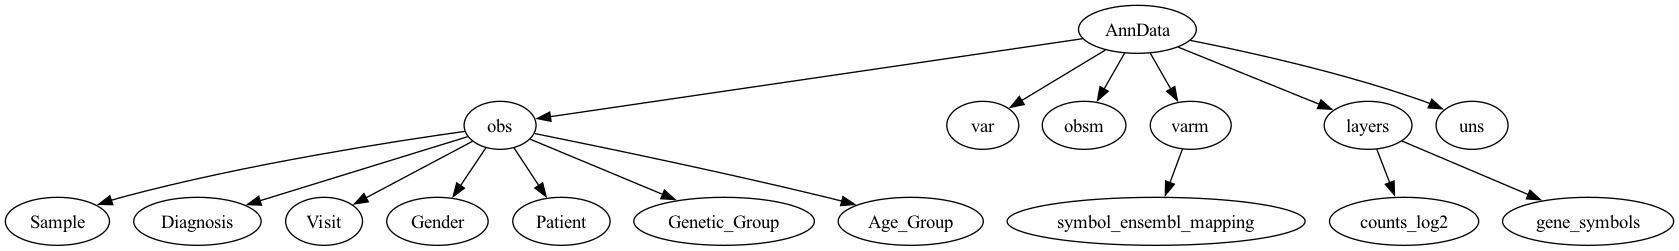
\includegraphics[width=0.8\textwidth]{anndata_structure.png}
                \caption{Δομή του AnnData αντικειμένου της εργασίας}
                \label{fig:figure-1}
            \end{figure}
    \section{Χρήση στατιστικών και βιοπληροφοριακών μεθόδων}
        \par
            Το σύνολο των δεδομένων που επιλέχθηκε σε αυτή την εργασία περιέχει μερικές αξιοσημείωτες προκλήσεις για την ανάλυση. Αφενός, αυτές προκύπτουν από τη φύση των δειγμάτων αίματος, όπου η ποικιλία μεταγραφικού προϊόντος είναι πιθανόν να εμπεριέχει και βιολογικό θόρυβο, ο οποίος δύναται να υπερκαλύπτει τυχόν σχετική με τη νόσο του Πάρκινσον πληροφορία. Αφετέρου, η ηλικία και το φύλο μπορεί να συμβάλουν σημαντικά σε μία διαφοροποίηση των δειγμάτων με χρήση στατιστικών μεθόδων ή αλγορίθμων μηχανικής μάθησης. Επιπλέον, τα άτομα που συμμετείχαν στη μελέτη κλήθηκαν σε επανειλημμένη δειγματοληψία, συνολικά σε πέντε επισκέψεις, σε απόσταση δύο μηνών από την προηγούμενη. Εξ αυτού κρίθηκε αναγκαία η στρωματοποίηση (\emph{Stratification}) των δειγμάτων σύμφωνα με το φύλο, την ηλικία αλλά και τις επισκέψεις.
        \par
            Με στόχο την λεπτομερή ανάλυση της γονιδιακής έκφρασης για την εξερεύνηση πιθανών λειτουργικών δικτύων, καθιερώθηκε πρωτόκολλο ανάλυσης αποτελούμενο από:
            \begin{enumerate}
                \item Την ανάλυση κυρίων συνιστωσών PCA\nomenclature{PCA}{Principal Component Analysis}, για την εξερεύνηση των δεδομένων, σύμφωνα με διαφορετικούς παράγοντες που πιθανώς επηρεάζουν τις τιμές έκφρασης.
                \item Την ανάλυση διαφορικής έκφρασης ανά στρώμα, για την ανάδειξη διαφορικά εκφραζόμενων γονιδίων.
                \item Την εφαρμογή ευρέως διαδομένων αλγορίθμων μηχανικής μάθησης στους τομείς της βιοπληροφορικής και την εξαγωγή χαρακτηριστικών που κρίθηκαν από τον εκάστοτε αλγόριθμο ως σημαντικά για την κατηγοριοποίηση.
                \item Την εφαρμογή της ανάλυσης εμπλουτισμού GSEA\nomenclature{GSEA}{Gene Set Enrichment Analysis} σε γονίδια που αναγνωρίστικαν ως διαφορικά εκφραζόμενα και σε αυτά που χαρακτηρίστικαν σημαντικά κατά την καηγοριοποίηση.
                \item Την αποτίμηση και σύκγριση των αποτελεσμάτων της ανάλυσης διαφορικής έκφρασης και της μηχανικής μάθησης.
                \item Την ανάλυση και κατασκευή/οπτικοποίηση πιθανών δικτύων συνέκφρασης σε γονίδια που βρέθηκαν ως διαφορικά εκφραζόμενα καθώς και από την σημαντικότητα χαρακτηριστικών των αποτελεσμάτων των αλγόρίθμων μηχανικής μάθησης.
            \end{enumerate}
    \chapter{Ανάλυση των δεδομένων}
        \section{Χαρακτηρισμός του συνόλου δεδομένων}
        \par
            Στην εικόνα \ref{fig:ppmi-proportion-of-genders-absolute-and-per-cohort} παρουσιάζονται οι αριθμοί συμμετεχόντων από κάθε φύλο, ανεξάρτητα από την ομάδα και τον τελικό αριθμό δειγμάτων. Πλην δύο μόνο συμμετεχόντων αγνώστου φύλου, ο χαρακτηρισμός των υπολοίπων είναι πλήρης για κάθε ομάδα. Το γράφημα στα δεξιά παρουσιάζει την ποσοστιαία κατανομή των συμμετεχόντων ανά φύλο και ομάδα. Στο κάτω μέρος παρουσιάζονται οι αριθμοί συμμετεχόντων της κάθε ομάδας ανά επίσκεψη (\emph{Visit}). Στην παρούσα εργασία χρησιμοποιήθηκαν μόνο δείγματα των ομάδων PD \nomenclature{PD}{Parkinson's Disease} και Control. Το πλήθος συμμετεχόντων για αυτές τις δύο ομάδες παρουσιάζεται στο γράφημα κάτω δεξιά, όπου απεικονίζονται οι απόλυτοι αριθμοί ατόμων ανά ομάδα και επίσκεψη. Χαρακτηριστικό είναι ότι η ομάδα ελέγχου υστερεί σε πλήθος της ομάδας PD, γεγονός το οποίο πρέπει να λαμβάνεται υπόψη ιδιαίτερα στην μοντελοποίηση κατηγοριοποιητών μηχανικής μάθησης.
            \begin{figure}[h]
                \centering
                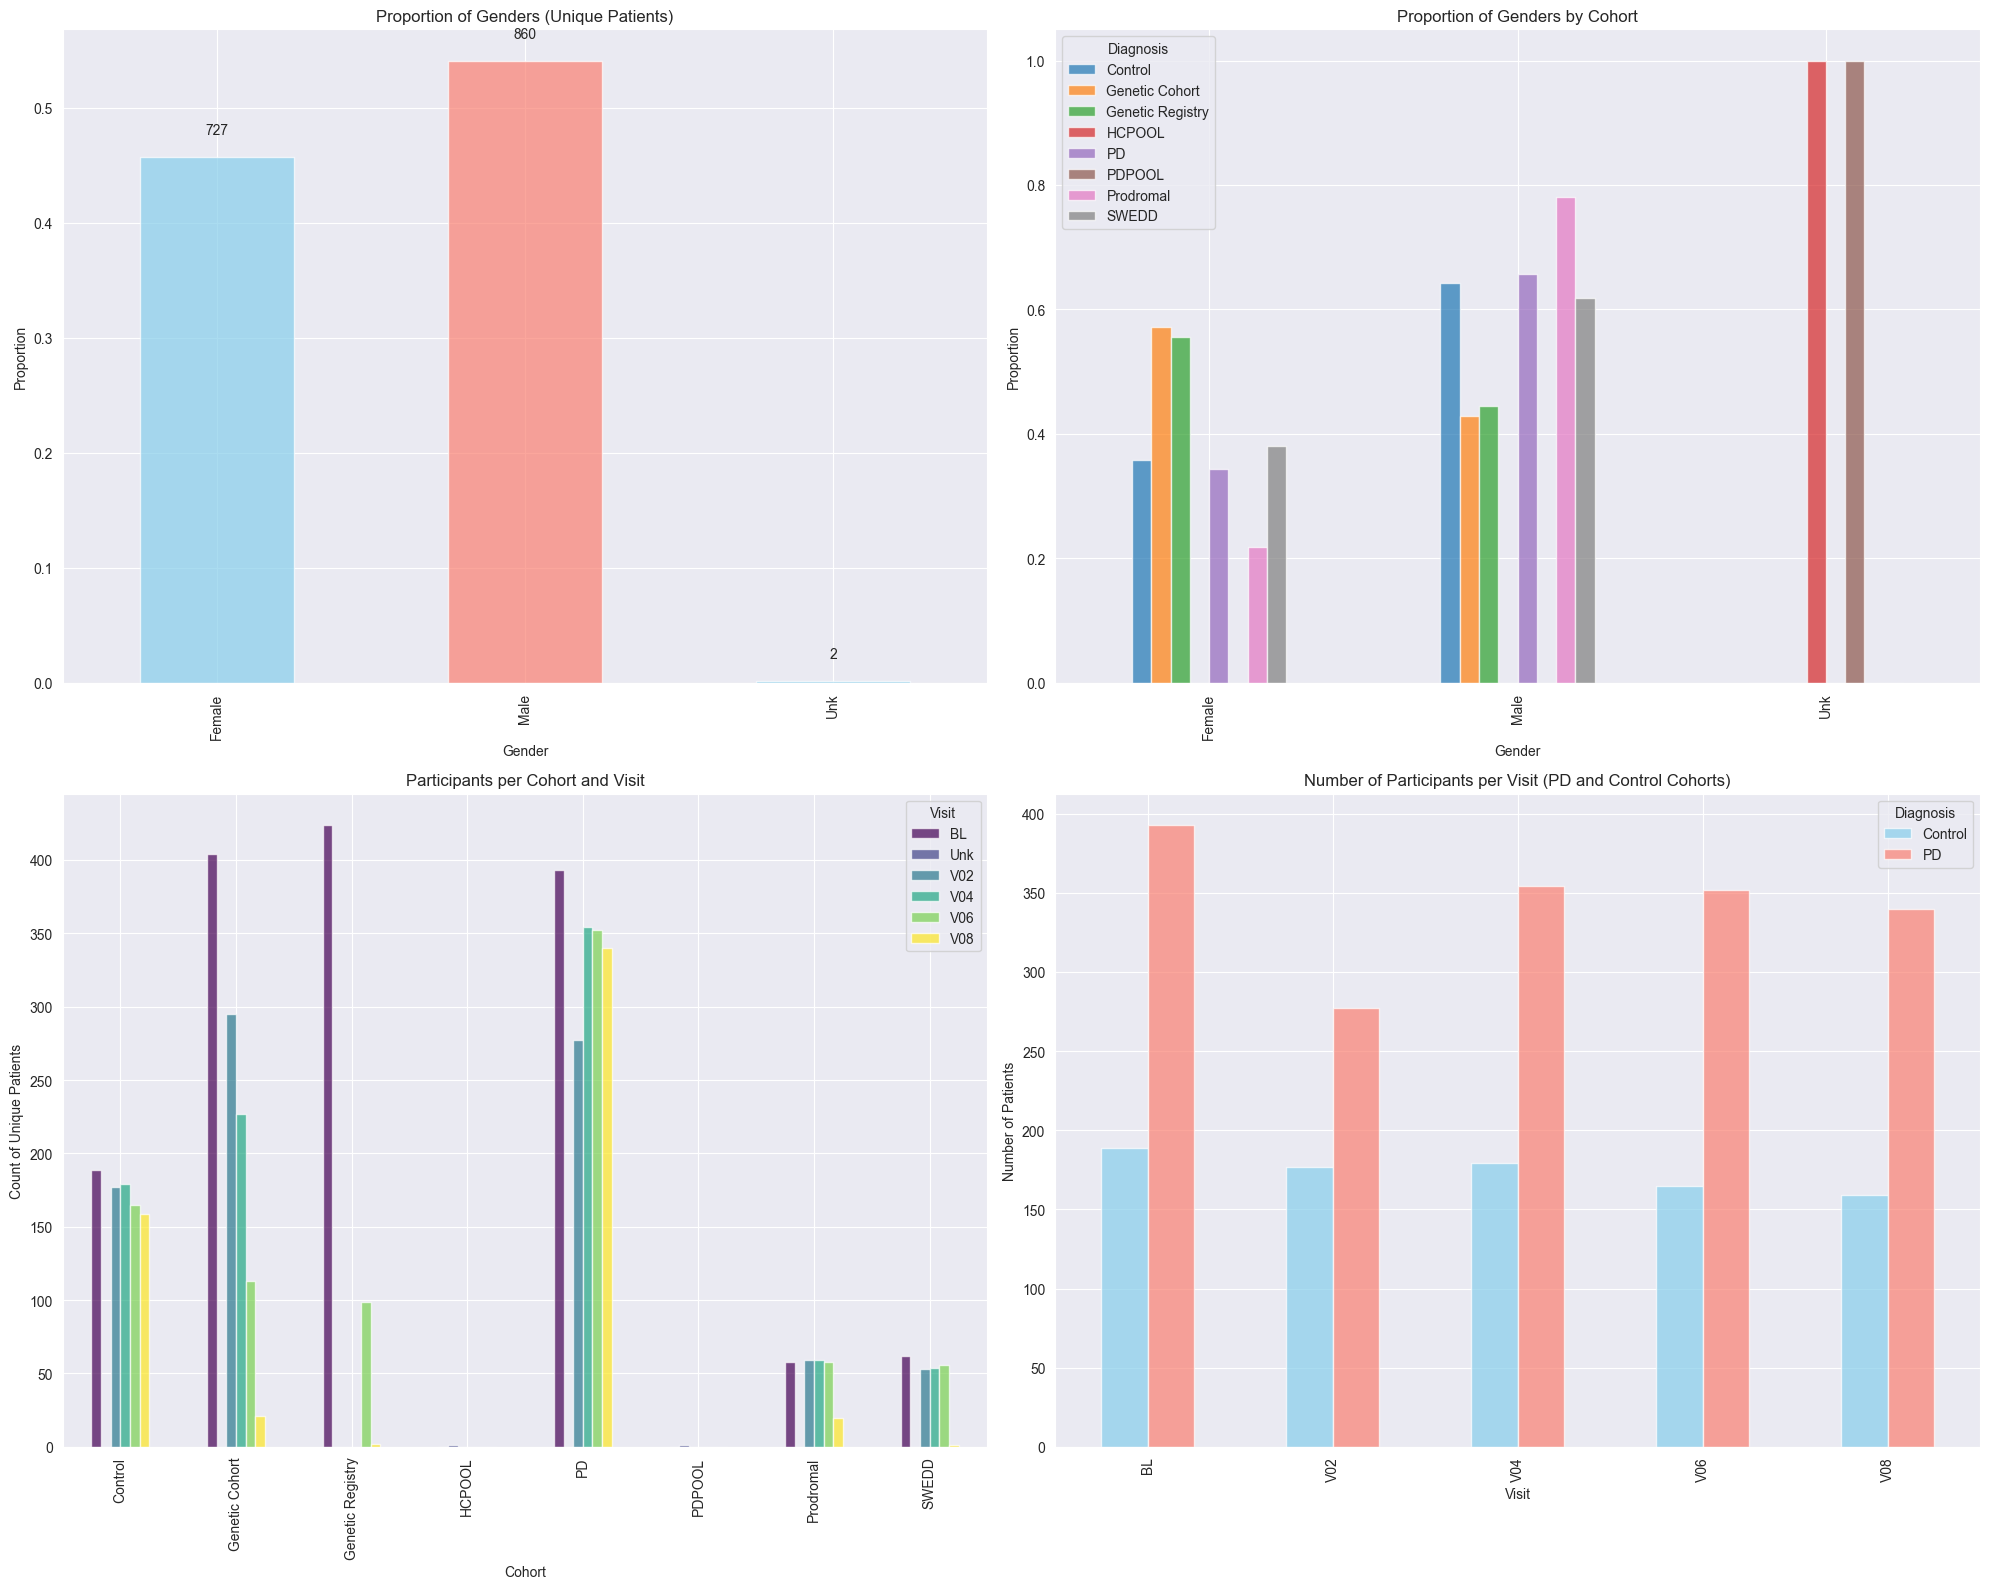
\includegraphics[width=0.73\linewidth]{Chapter-2-Section-2.1/ppmi-prop-gender-abs-per-cohort_samples-per-coh-visit-all-coh_pd-vs-ctrl.png}
                \caption[Πλήθος συμμετέχοντων ανά φύλο]{Επάνω αριστερά: Συμμετέχοντες ανά φύλο συνολικα, Επάνω δεξιά: Συμμετέχοντες ανά ομάδα. Κάτω αριστερά: Συμμετέχοντες ανά ομάδα και επίσκεψη. Κάτω δεξιά: Συμμετέχοντες ανά ομάδα και επίσκεψη.}
                \label{fig:ppmi-proportion-of-genders-absolute-and-per-cohort}
            \end{figure}
        \par
            Πρέπει να σημειωθεί ότι η αλληλούχιση διενεργήθηκε σε δύο διαφορετικές φάσεις. Αυτό δεν σημαίνει πως η δειγματοληψία ακολούθησε επίσης αυτόν τον διαχωρισμό, έτσι ώστε να προκύψουν για κάθε συμμετέχοντα δέκα δείγματα, ήτοι πέντε επισκέψεις επί δύο φάσεις, αλλά δείγματα από τις πέντε (\emph{ή και λιγότερες}) διαφορετικές επισκέψεις μπορεί να αλληλουχίστηκαν σε διαφορετικές φάσεις. Σαφώς αυτό καθιστά έναν τεχνικό παράγοντα που μπορεί να οδηγήσει σε ανακριβή αποτελέσματα σε αναλύσεις. Ειδικά η αλληλούχιση των δειγμάτων της δεύτερης επίσκεψης έχει γίνει αποκλειστικά στη δεύτερη φάση, σύμφωνα με την εικόνα~\ref{fig:ppmi-bars-pd-ctrl-visits-per-phase}. Ένα επίσης ερώτημα μπορεί να απαντηθεί ως προς το αν τα δείγματα όλων των ηλικιακών ομάδων εκπροσωπούνται και στις δύο φάσεις. Με το γράφημα στην εικόνα~\ref{fig:ppmi-bars-pd-ctrl-age_groups-per-phase} η απάντηση μπορεί να δοθεί καταφατικά, όπως επίσης και ότι δεν υπάρχει αξιοσημείωτη ασυμμετρία στην κατανομή των ηλικιακών ομάδων ανά φάση αλληλούχισης.

            \begin{figure}[ht]
                \centering
                \begin{subfigure}[b]{0.48\textwidth}
                    \centering
                    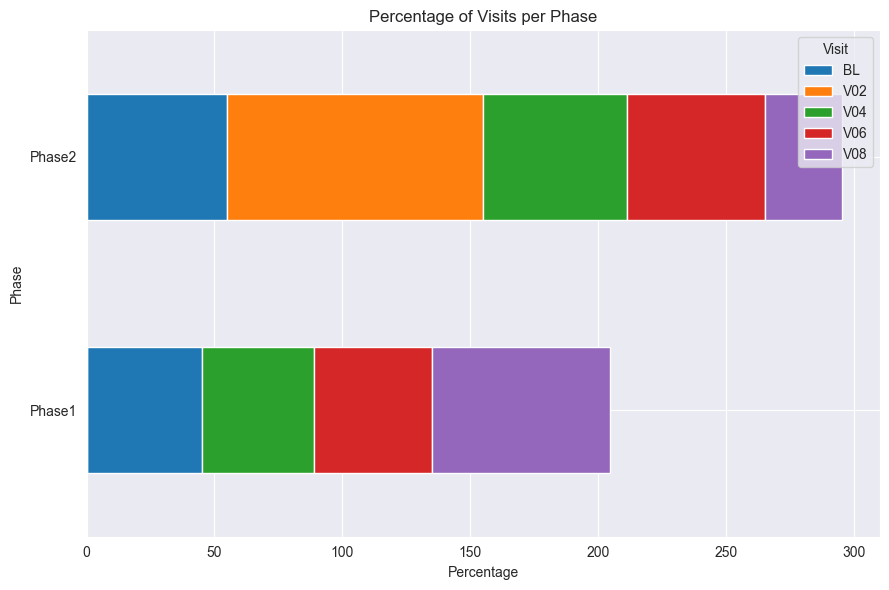
\includegraphics[width=\linewidth,height=7.5cm]{Chapter-2-Section-2.1/ppmi-bars-pd-ctrl-visits-per-phase.png}
                    \caption{Κατανομή δειγμάτων ανά επίσκεψη και φάση αλληλούχισης}
                    \label{fig:ppmi-bars-pd-ctrl-visits-per-phase}
                \end{subfigure}
                \hfill
                \begin{subfigure}[b]{0.48\textwidth}
                \centering
                    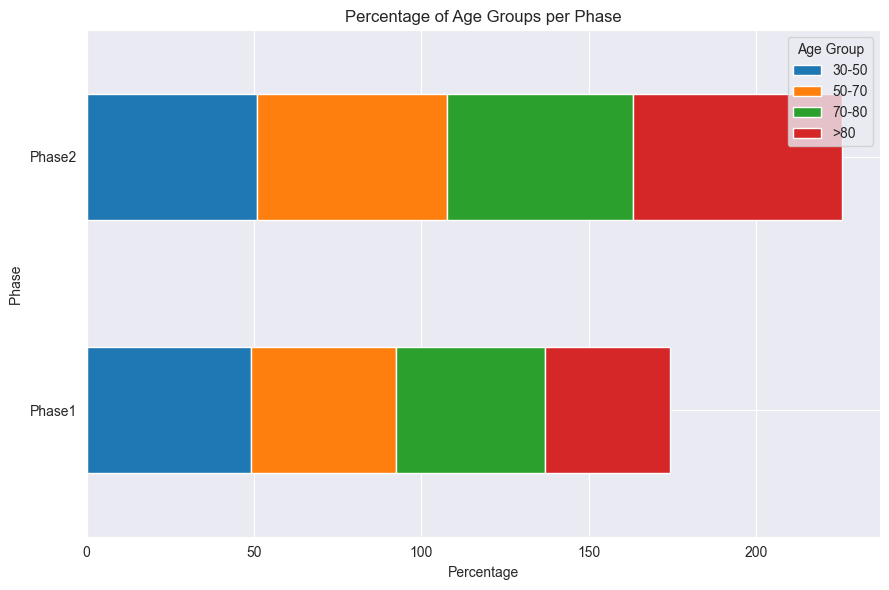
\includegraphics[width=\linewidth,height=7.5cm]{Chapter-2-Section-2.1/ppmi-bars-pd-ctrl-age_groups-per-phase.png}
                    \caption{Κατανομή ηλικιακών ομάδων ανά φάση αλληλούχισης}
                    \label{fig:ppmi-bars-pd-ctrl-age_groups-per-phase}
                \end{subfigure}
                \label{fig:ppmi-visit-phase-sample-distributions}
                \caption{Οπτικοποίηση δειγμάτων ανά φάση αλληλούχισης}
            \end{figure}
        \newpage

        \section{Ανάλυση κυρίων συνιστωσών}
            \par
                Στην εικόνα \ref{fig:ppmi-pca-pd-ctrl-all-visits-hue_diagnosis} παρουσιάζεται το αποτέλεσμα της PCA για τις πρώτες πέντε συνιστώσες, όπου ο χρωματισμός πραγματοποιήθηκε σύμφωνα με τη διάγνωση. Δεν διακρίνονται ξεχωριστές συστάδες, γεγονός που συνιστά πως η μεταβλητότητα των εκφράσεων δεν διαχωρίζει σε αυτό το επίπεδο ανάλυσης δείγματα νοσούντων από υγιείς. Ενδιαφέρουσα είναι η απεικόνιση κυρίων συνιστωσών με χρωματισμό με βάση το φύλο, όπου διακρίνονται συστάδες μεταξύ της πέμπτης συνιστώσας και όλων των υπολοίπων. Το συμπέρασμα είναι πως υπάρχει μεταβλητότητα σύμφωνα με γονιδιακές εκφράσεις στα δείγματα ολικού αίματος, με την οποία δύναται να διακριθούν τα δείγματα των δύο φύλων. Πρόκειται για πολύ μικρό μέρος εκ του συνόλου της μεταβλητότητας (\emph{Πίνακας~\ref{tab:pca}}). Η στρωμάτωση των δειγμάτων σε παρακάτω βήματα χρησιμεύει προς αποφυγήν της όποιας πιθανής παρεμβολής στις διάφορες αναλύσεις.

            \begin{figure}[ht]
                \centering
                \begin{subfigure}[b]{0.48\textwidth}
                    \centering
                    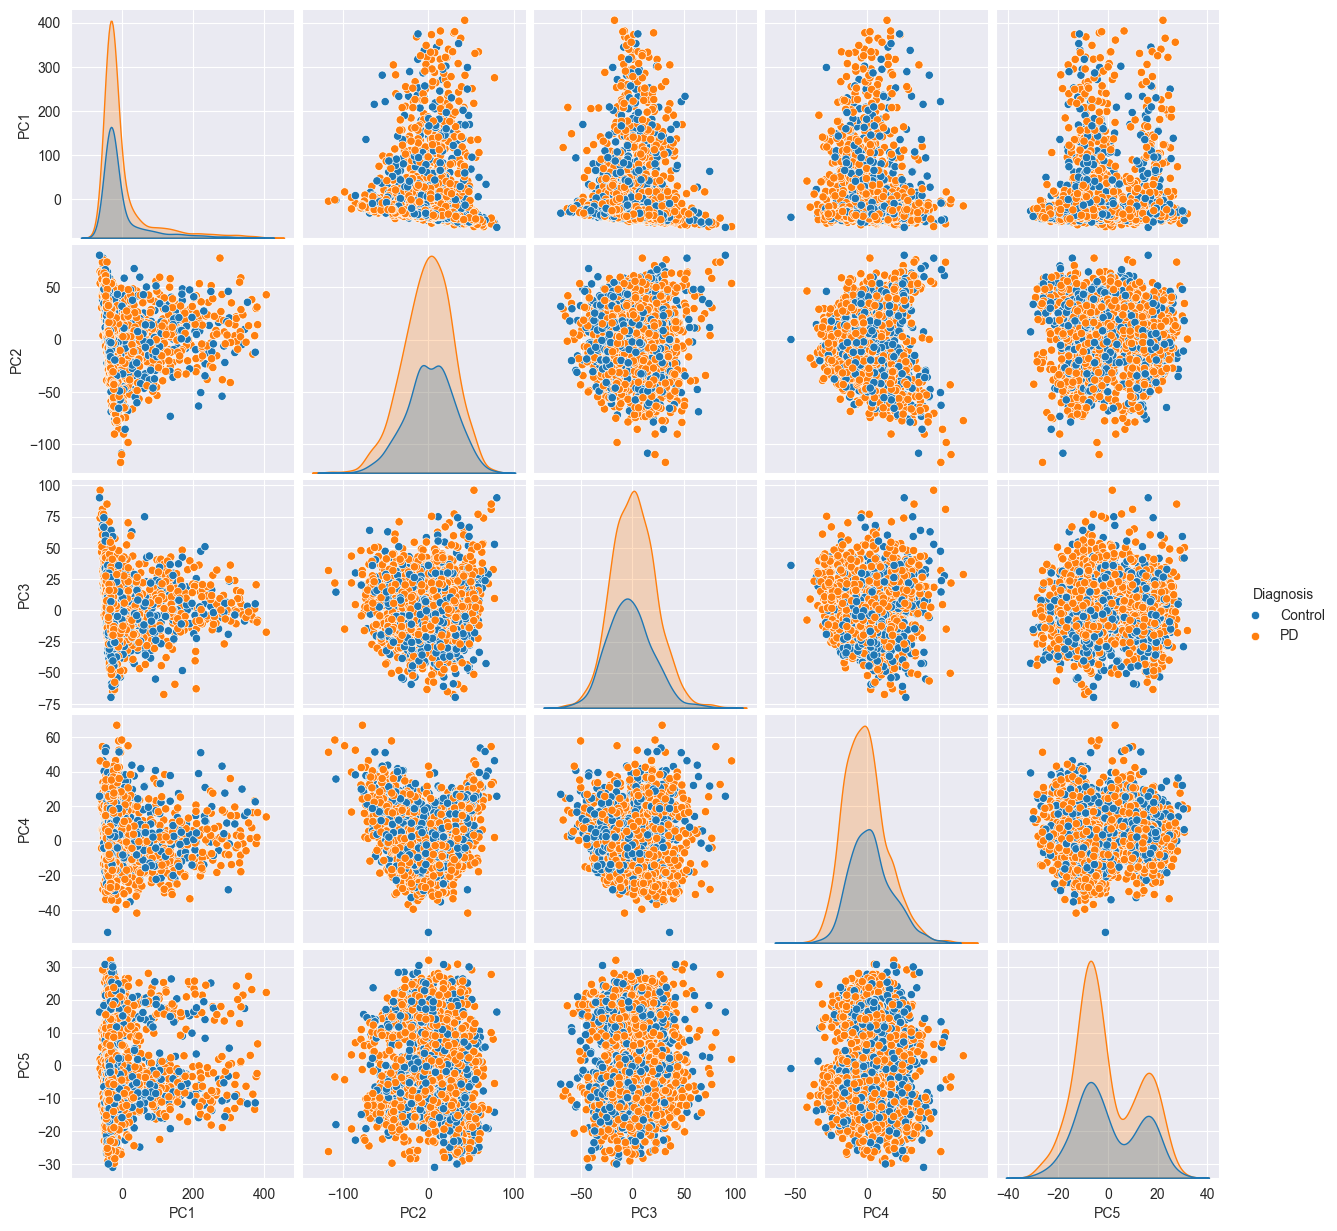
\includegraphics[width=\linewidth,height=7cm]{Chapter-2-Section-2.1/ppmi-pca-pd-ctrl-all-visits-hue_diagnosis.png}
                    \caption{PCA σύμφωνα με την διάγνωση}
                    \label{fig:ppmi-pca-pd-ctrl-all-visits-hue_diagnosis}                
                \end{subfigure}
                \hfill
                \begin{subfigure}[b]{0.48\textwidth}
                    \centering
                    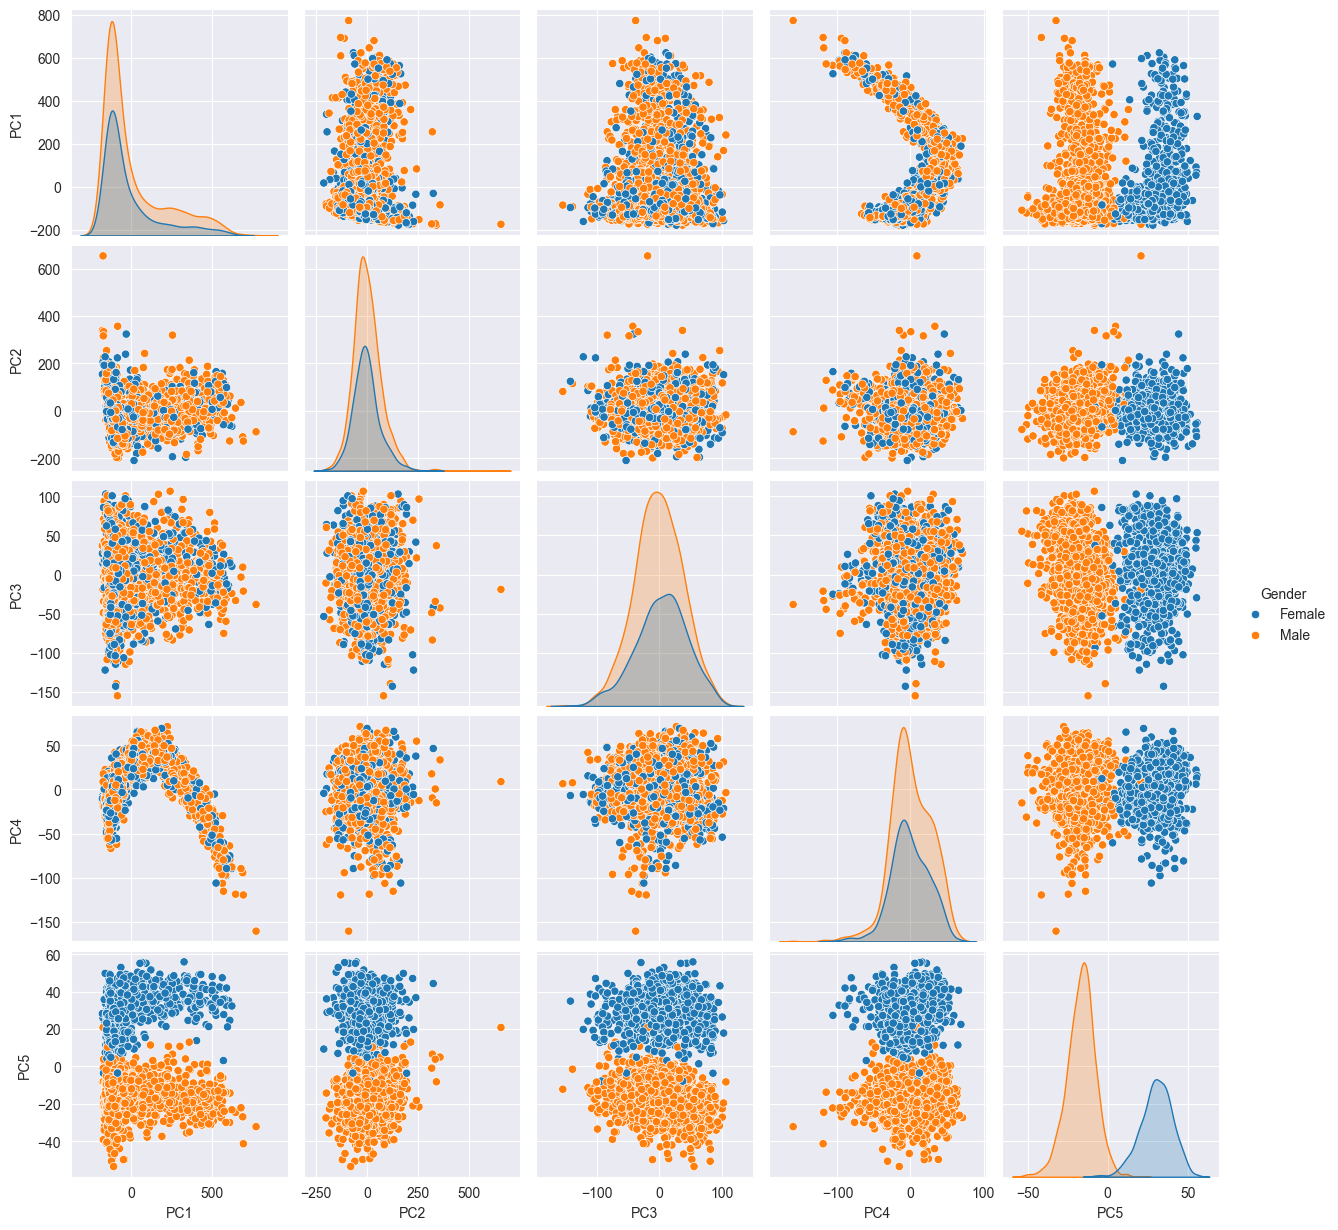
\includegraphics[width=\linewidth,height=7cm]{Chapter-2-Section-2.1/ppmi-pca-pd-ctrl-all-visits-hue_gender.png}
                    \caption{PCA σύμφωνα με τo φύλο}
                    \label{fig:ppmi-pca-pd-ctrl-all-visits-hue_gender}    
                \end{subfigure}
                \label{fig:ppmi-pca-scatterplot}
                \caption{Αποτελέσματα PCA}
            \end{figure}

            \begin{table}[ht]
                \centering
                \caption{Μεταβλητότητα ανά συνιστώσα}
                \begin{tabular}{lcccc} % No vertical lines
                    \toprule
                    \textbf{PC 1} & \textbf{PC 2} & \textbf{PC 3} & \textbf{PC 4} & \textbf{PC 5} \\
                    \midrule
                    56,88\% & 8,77\% & 5,15\% & 2,44\% & 1,78\% \\
                    \bottomrule
                \end{tabular}
                \label{tab:pca}
            \end{table}
            \newpage
            \par
                Παρακάτω απεικονίζεται το αποτέλεσμα της PCA σύμφωνα με τη φάση αλληλούχισης. Εντός των πρώτων πέντε κύριων συνιστωσών δεν παρατηρείται ομαδοποίηση και μαζί με αυτό προκύπτει και η διαβεβαίωση πως δεν εισάγεται τεχνικός θόρυβος από τη φάση αλληλούχισης.
                \begin{figure}[H]
                    \centering
                    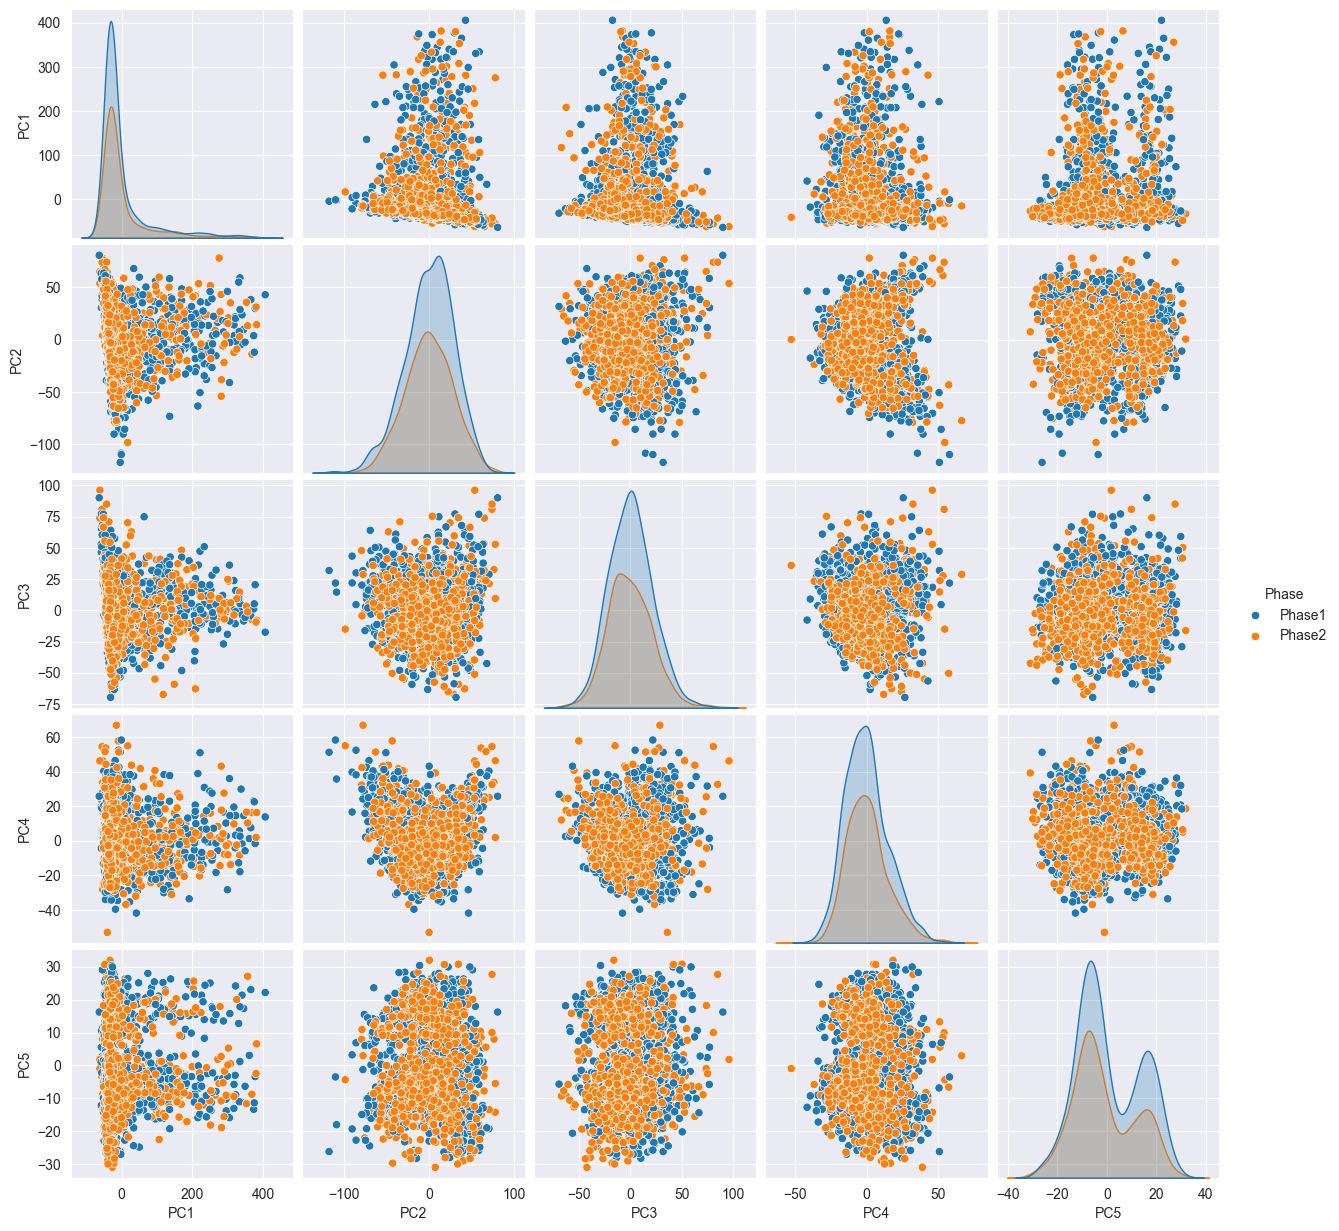
\includegraphics[width=0.75\textwidth]{Chapter-2-Section-2.1/ppmi-pca-pd-ctrl-all-visits-hue-phase.png}
                    \caption{PCA σύμφωνα με τη φάση αλληλούχισης}
                    \label{fig:ppmi-pca-pd-ctrl-all-visits-hue-phase}
                \end{figure}
    \section{Ανάλυση διαφορικής γονιδιακής έκφρασης}
        \par
            Η ανάλυση διαφορικής έκφρασης (\emph{DGEA\nomenclature{DGEA}{Differential Gene Expression Analysis}}) διενεργήθηκε μετά από στρωματοποίηση των δειγμάτων σύμφωνα με το φύλο και την ηλικιακή ομάδα με τη χρήση του πακέτου λογισμικού της R, DESeq2 (\emph{\cite{Love2014ModeratedDESeq2}}) (\emph{κώδικας~\ref{lst:mainr}}) και αντίστοιχη οπτικοποίηση με χρήση σεναρίου στην γλώσσα Python (\emph{κώδικας~\ref{lst:processdegconsolidatedvisitspy}}). Η επίσκεψη της κάθε δειγματοληψίας συμπεριλήφθηκε ως συμμεταβλητή και θεωρήθηκε ως τεχνικός παράγοντας, χωρίς να ερευνηθεί αν έχει βιολογικό χαρακτήρα ως προς την πρόοδο της νόσου. Ως όριο για την έκφραση $|log_2FoldChange|$ τέθηκε η τιμή $>0,5$ ενώ για την τιμή της $padj<0,05$.
        \par
            Το αντίστοιχο τμήμα της διαδικασίας ανάλυσης (\emph{Pipeline}) παρουσιάζεται στην εικόνα~\ref{fig:msci-big-pic-DEGs-blocks}. Το κομμάτι αυτό κατακερματίζει το σύνολο δεδομένων σύμφωνα με το φύλο και την ηλικιακή ομάδα των συμμετεχόντων σε υποσύνολα, όπου για κάθε υποσύνολο διεξάγεται η διαφορική ανάλυση μέσω DESeq2. Πέραν της διάγνωσης, συμπεριλήφθηκε και η παρατήρηση των επισκέψεων δειγματοληψίας (\emph{Visit}), καθώς καθιστά πηγή μεταβλητότητας η οποία πρέπει να ληφθεί υπόψη ως τεχνικός παράγοντας στην στατιστική ανάλυση (\emph{\cite{Love2016DifferentialPackage}}).
        \par
            Τα αποτελέσματα περιέχουν τα διαφορικά εκφραζόμενα και καταγράφονται σε μορφή CSV σε διαφορετικά αρχεία για περαιτέρω ανάλυση.
            \begin{figure}[h]
                \centering
                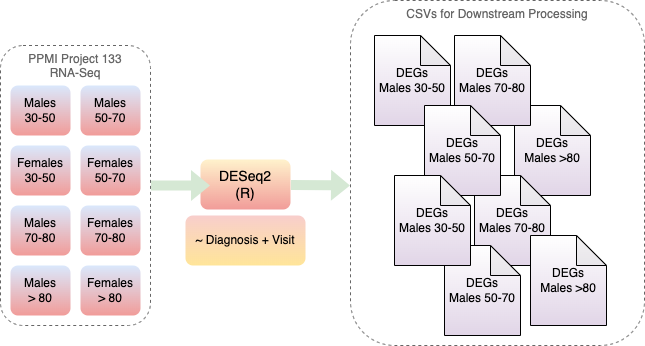
\includegraphics[width=0.7\textwidth]{Chapter-3/msci-big-pic-DEGs-blocks.png}
                \caption{Pipeline για την ανάλυση διαφορικής έκφρασης με εξαγωγή αποτελεσμάτων σε αρχεία CSV}
                \label{fig:msci-big-pic-DEGs-blocks}
            \end{figure}
        \subsection{Διαφορική έκφραση γονιδίων σε γυναίκες}
         \par
            Το πλήθος των στατιστικά σημαντικών εκφραζόμενων γονιδίων ποικίλει ανά ηλικιακή ομάδα. Στη σειρά διαγραμμάτων της εικόνας~\ref{fig:volcano_plot_consoVisits_Female} διακρίνονται περισσότερα γονίδια στατιστικής σημασίας στην ηλικιακή ομάδα 30-50 έναντι της ομάδας 50-70 ετών. Ενδεχομένως η νόσος να διαφοροποιείται σε γονιδιακό επίπεδο σε περιπτώσεις όπου η νόσος εκδηλώνεται σε μικρότερες ηλικίες. Σε ηλικίες άνω των 70 ετών το πλήθος των διαφορικά εκφραζόμενων γονιδίων στατιστικής σημασίας αυξάνεται σημαντικά, κάτι που μπορεί να παραπέμπει και στην πρόοδο της νόσου με αυξανόμενη ηλικία. Όσον αφορά το πλήθος των υπέρ-έναντι των υπό-εκφραζόμενων γονιδίων, ισχύει σύμφωνα με την παρακάτω οπτικοποίηση στην εικόνα~\ref{fig:barplot_plot_consoVisits_Female}, ότι υπάρχουν περισσότερα υπέρ-εκφραζόμενα γονίδια σε όλες τις ηλικιακές ομάδες υπό παρατήρηση.
            \begin{figure}[h]
                \centering
                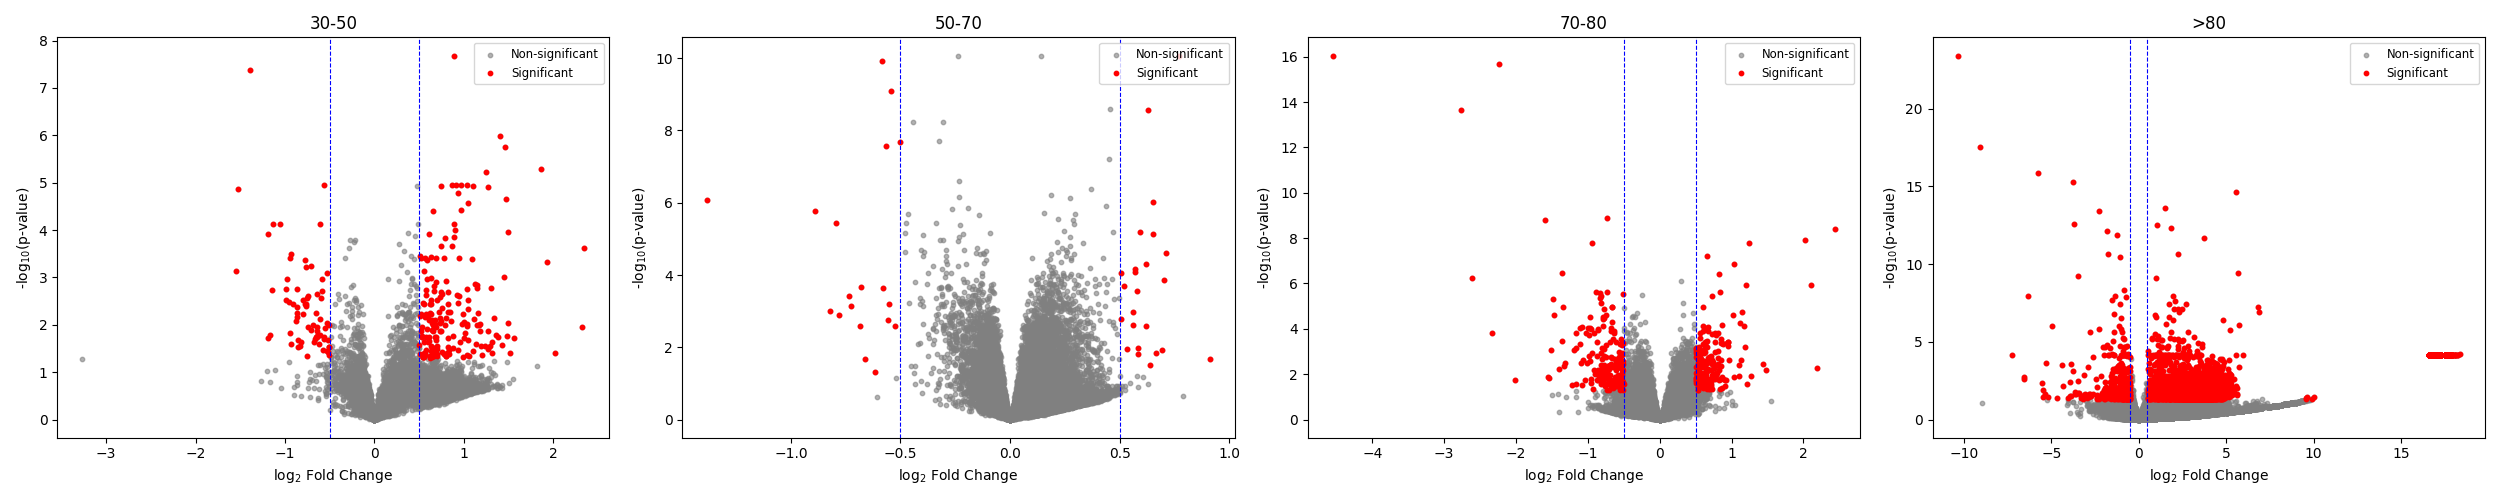
\includegraphics[width=\textwidth,height=4cm]{Chapter-3/volcano_plot_consoVisits_Female.png}
                \caption{Διαγράμματα Ηφαιστείου ανά ηλικιακή ομάδα γυναικών}
                \label{fig:volcano_plot_consoVisits_Female}
            \end{figure}
            \begin{figure}[H]
                \centering
                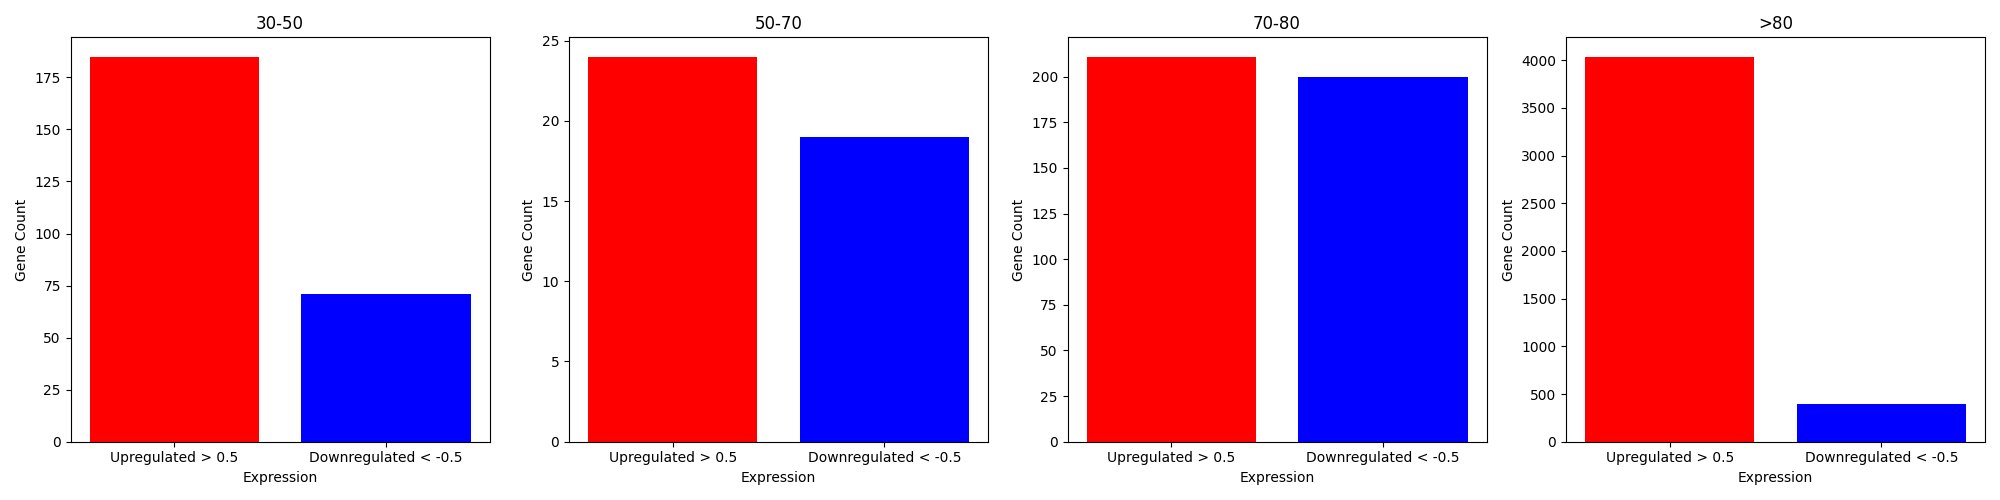
\includegraphics[width=\textwidth,height=4cm]{Chapter-3/barplot_plot_consoVisits_Female.png}
                \caption{Πλήθος στατιστικά σημαντικών διαφορικά εκφραζόμενων γονιδίων - Γυναίκες}
                \label{fig:barplot_plot_consoVisits_Female}
            \end{figure}

        \subsection{Διαφορική έκφραση γονιδίων σε άνδρες}
        \par
            Συνολικά η διαφορική έκφραση γονιδίων στους άνδρες σε κάθε ηλικιακή ομάδα διαφέρει από τις εκφράσεις των γυναικών. Χαρακτηριστική είναι η παρουσία περισσότερων υπέρ-εκφραζόμενων γονιδίων έναντι ελάχιστων υπό-εκφραζόμενων στην ηλικιακή ομάδα των 50-70, ενώ στις υπόλοιπες περιπτώσεις ο αριθμός των υπό-εκφραζόμενων δείχνει να είναι περίπου διπλάσιος από των υπέρ-εκφραζόμενων.
            \begin{figure}[h]
                \centering
                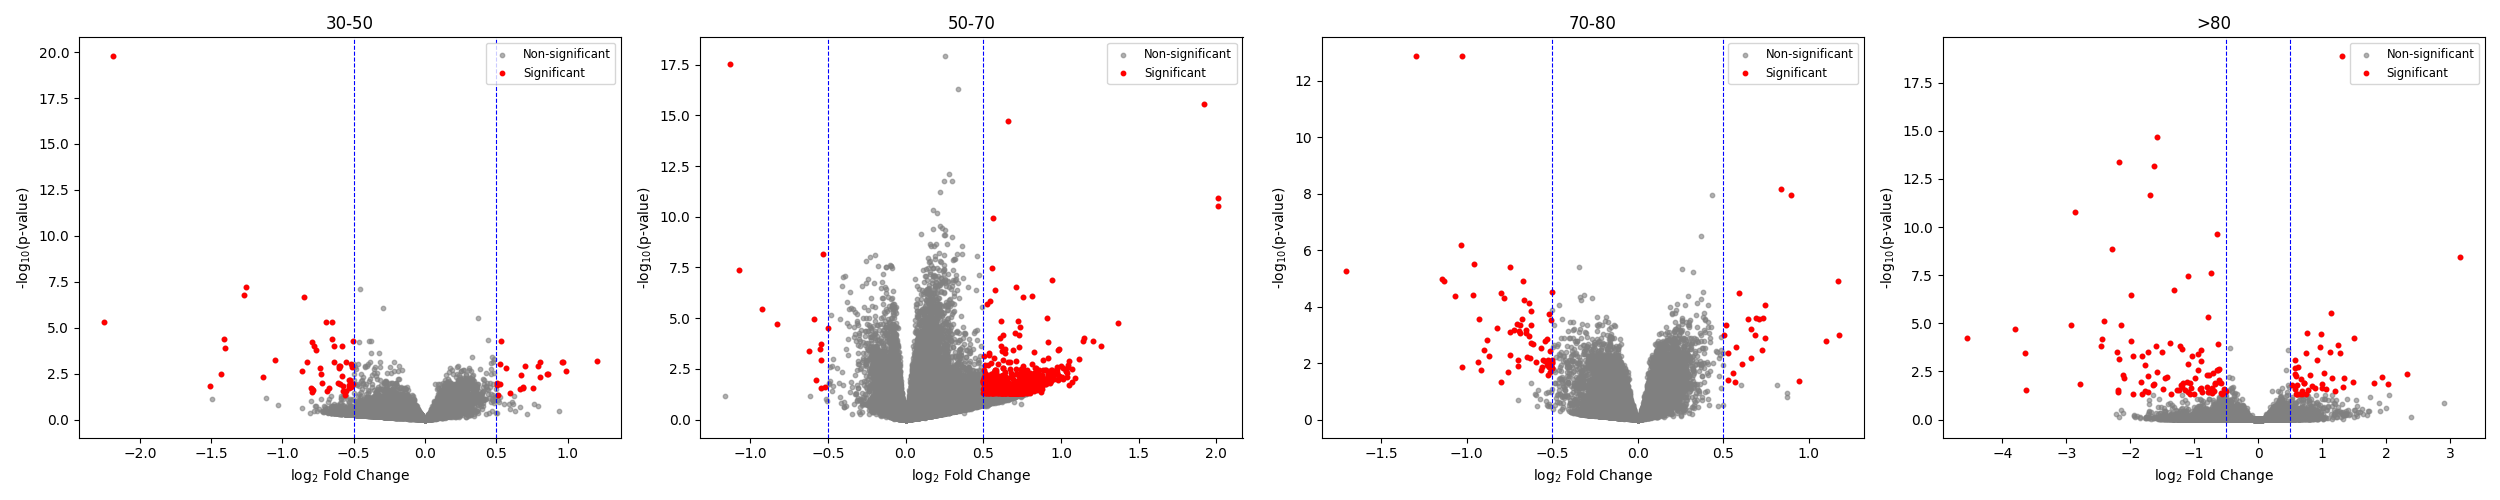
\includegraphics[width=\textwidth,height=4cm]{Chapter-3/volcano_plot_consoVisits_Male.png}
                \caption{Διαγράμματα Ηφαιστείου ανά ηλικιακή ομάδα ανδρών}
                \label{fig:volcano_plot_consoVisits_Male}
            \end{figure}
            \begin{figure}[H]
                \centering
                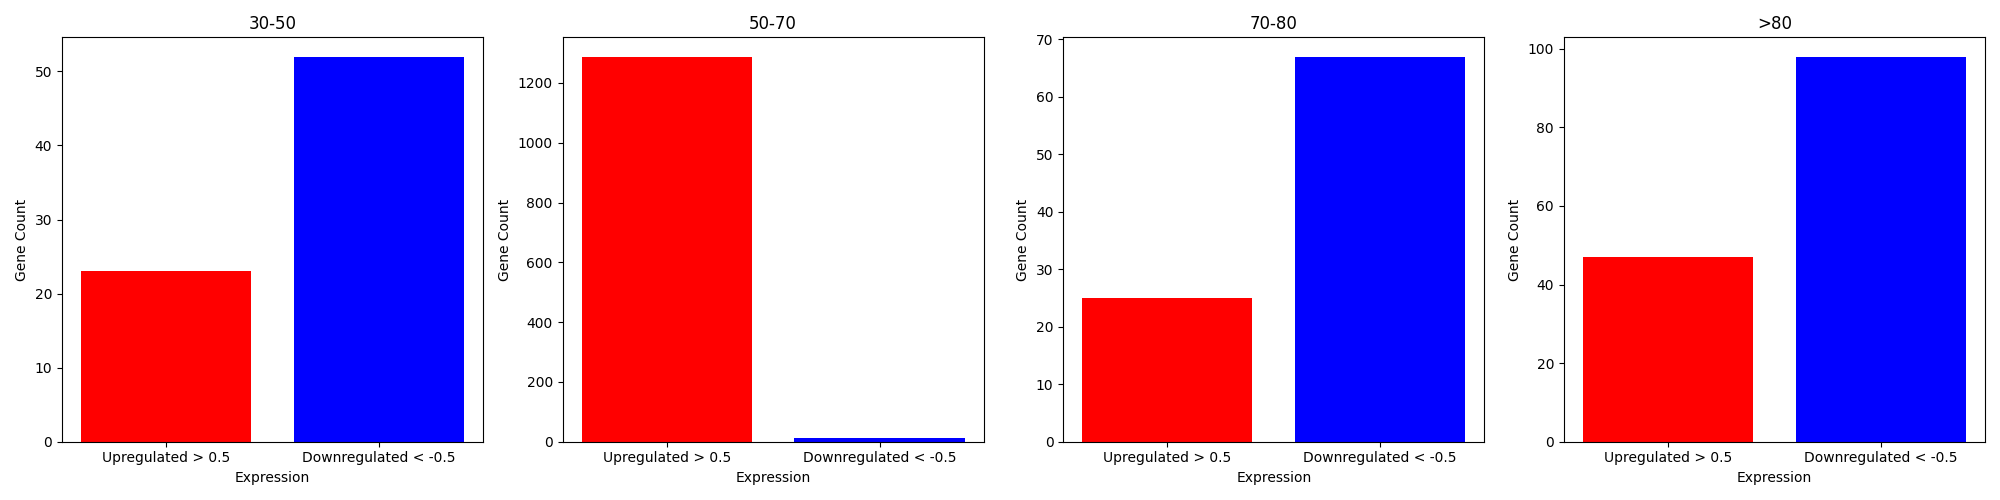
\includegraphics[width=\textwidth,height=4cm]{Chapter-3/barplot_plot_consoVisits_Male.png}
                \caption{Πλήθος στατιστικά σημαντικών διαφορικά εκφραζόμενων γονιδίων - Άνδρες}
                \label{fig:barplot_plot_consoVisits_Male}
            \end{figure}
        \subsection{Σύνοψη της ανάλυσης διαφορικής έκφρασης}
            \par
                Τα αποτελέσματα ανά φύλο και ηλικιακή ομάδα διαφέρουν σε αριθμούς υπό- και υπέρ-εκφραζόμενων γονιδίων. Μια σύντομη σύνοψη των πρώτων έξι διαφορικά εκφραζόμενων γονιδίων παρουσιάζεται στον πίνακα~\ref{tab:top-6-degs-strata}. Πρόκειται για τα γονίδια που έχουν τις χαμηλότερες τιμές $padj$ καθώς και τις υψηλότερες απόλυτες τιμές $log_2FoldChange$.
                \begin{table}[ht]
                    \centering
                    \caption[Ενδεικτική επιλογή έξι διαφορικά εκφραζόμενων γονιδίων] {Ενδεικτική επιλογή έξι διαφορικά εκφραζόμενων γονιδίων με υψηλότερη απόλυτη τιμή έκφρασης και υψηλή στατιστική σημαντικότητα. Υπέρ-εκφραζόμενα γονίδια παρουσιάζονται με κόκκινο φόντο, υπό-εκφραζόμενα με μπλε. Κοινά γονίδια παρουσιάζονται \textbf{έντονα} και \underline{υπογραμμισμένα}}
                    \small
                    \setlength{\tabcolsep}{5pt}
                    \renewcommand{\arraystretch}{1.4}
                    \begin{tabular}{@{}>{\raggedright}p{1.3cm}cccc@{}}
                        \toprule
                        \textbf{Φύλο} & \textbf{30-50} & \textbf{50-70} & \textbf{70-80} & \textbf{>80} \\
                        \midrule
                        \multirow{6}{*}{'Ανδρες}
                        & \cellcolor{blue!20}\textbf{\underline{RNU671-P}} & \cellcolor{red!20}NFYAP1 & \cellcolor{blue!20}\textbf{\underline{RNU1-67P}} & \cellcolor{blue!20}LINC02506 \\
                        & \cellcolor{blue!20}CNTNAP3P2 & \cellcolor{red!20}ENSG00000270962 & \cellcolor{blue!20}NECTIN2 & \cellcolor{blue!20}ENSG00000276345 \\
                        & \cellcolor{blue!20}RNU1-83P & \cellcolor{red!20}LINC00355 & \cellcolor{red!20}\textbf{\underline{ENSG00000259385}} & \cellcolor{blue!20}DEFA3 \\
                        & \cellcolor{blue!20}TUSC3 & \cellcolor{red!20}TRIM64 & \cellcolor{red!20}LRRC37A2 & \cellcolor{blue!20}\textbf{\underline{ENSG00000223779}} \\
                        & \cellcolor{blue!20}LINC02470 & \cellcolor{red!20}ANKRD33BP9 & \cellcolor{blue!20}IFI44L & \cellcolor{red!20}\textbf{\underline{HLA-DQA2}} \\
                        & \cellcolor{blue!20}TUBB2B & \cellcolor{red!20}LCEP2 & \cellcolor{blue!20}CYP4F29P & \cellcolor{blue!20}PAX8-AS1 \\
                        \midrule
                        \multirow{6}{*}{Γυναίκες}
                        & \cellcolor{red!20}RNVU1-7 & \cellcolor{blue!20}\textbf{\underline{RNU1-67P}} & \cellcolor{blue!20}DCLRE1CP1 & \cellcolor{red!20}REXO1L10P \\
                        & \cellcolor{red!20}CTAG2 & \cellcolor{red!20}ADAD1P1 & \cellcolor{blue!20}LINC02899 & \cellcolor{red!20}MIR4289 \\
                        & \cellcolor{red!20}ADGRG7 & \cellcolor{blue!20}RAP1GAP & \cellcolor{blue!20}\textbf{\underline{HLA-DQA2}} & \cellcolor{red!20}ENSG00000241573 \\
                        & \cellcolor{red!20}MRPS35-DT & \cellcolor{blue!20}\textbf{\underline{ENSG00000259385}} & \cellcolor{red!20}C4BPA & \cellcolor{red!20}IQCJ-SCHIP1-AS1 \\
                        & \cellcolor{red!20}ENSG00000275649 & \cellcolor{blue!20}ENSG00000265218 & \cellcolor{blue!20}CEACAMP3 & \cellcolor{red!20}ENSG00000238140 \\
                        & \cellcolor{red!20}\textbf{\underline{ENSG00000223779}} & \cellcolor{blue!20}CTXN2-AS1 & \cellcolor{blue!20}AGAP12P & \cellcolor{red!20}ENSG00000236046 \\
                        
                        \bottomrule
                    \end{tabular}
                    \label{tab:top-6-degs-strata}
                \end{table}
                \par
                    Στην εικόνα~\ref{fig:common-genes-across-genders-per-age-group} παρατίθενται στα εξής διαγράμματα κοινά γονίδια μεταξύ των φύλων ανά ηλικιακή ομάδα, στατιστικά σημαντικά και με τιμές έκφρασης $|log_2FoldChange| > 0,5$. Από τα κοινά γονίδια υπάρχουν μόνο λίγα που παρουσιάζουν ίδιο πρότυπο έκφρασης, δηλαδή είτε και στα δυο φύλα να υπέρ- ή να υπό-εκφράζονται (\emph{υπέρ-εκφραζόμενα γονίδια με κόκκινο και υπό-εκφραζόμενα με μπλε χρώμα. Η τιμή έκφρασης αντικατοπτρίζεται από το μέγεθος των κύκλων}).
                    \begin{figure}[ht]
                        \centering
                        \begin{subfigure}[b]{0.48\textwidth}
                            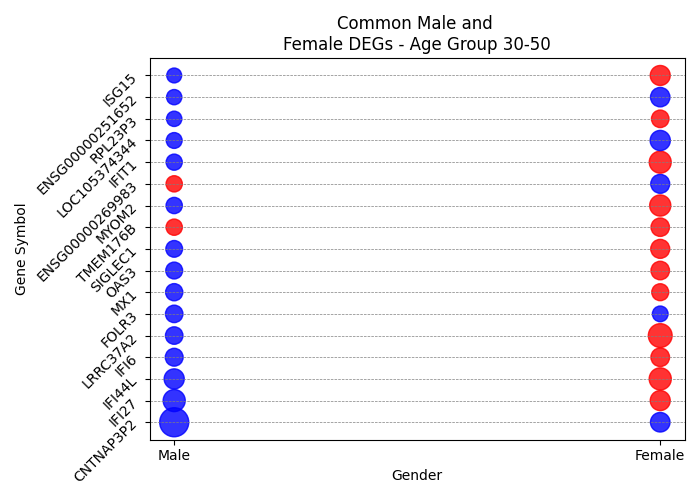
\includegraphics[width=\textwidth]{Chapter-3/bubbleplot_combined_30-50.png}
                            \caption{Κοινά διαφορικά εκφραζόμενα γονίδια ηλικίας 30-50}
                            \label{fig:bubbleplot_combined_30-50}
                        \end{subfigure}
                        \hfill % Add horizontal fill
                        \begin{subfigure}[b]{0.48\textwidth}
                            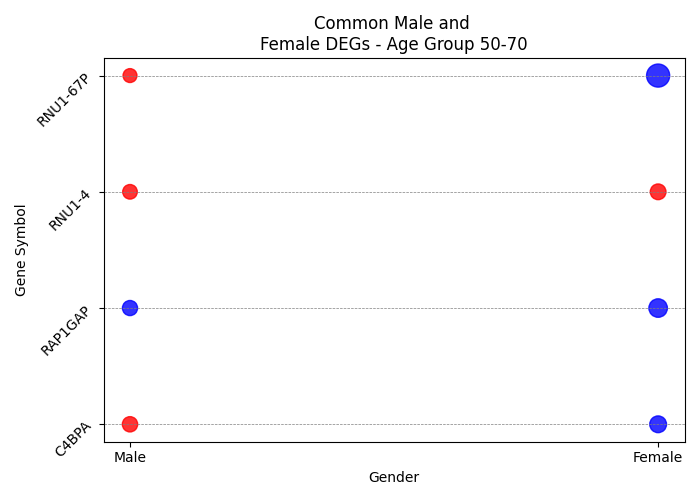
\includegraphics[width=\textwidth]{Chapter-3/bubbleplot_combined_50-70.png}
                            \caption{Κοινά διαφορικά εκφραζόμενα γονίδια ηλικίας 50-70}
                            \label{fig:bubbleplot_combined_50-70}
                        \end{subfigure}
                        
                        \vspace{0.5cm} % Vertical spacing between rows
                        
                        \begin{subfigure}[b]{0.48\textwidth}
                            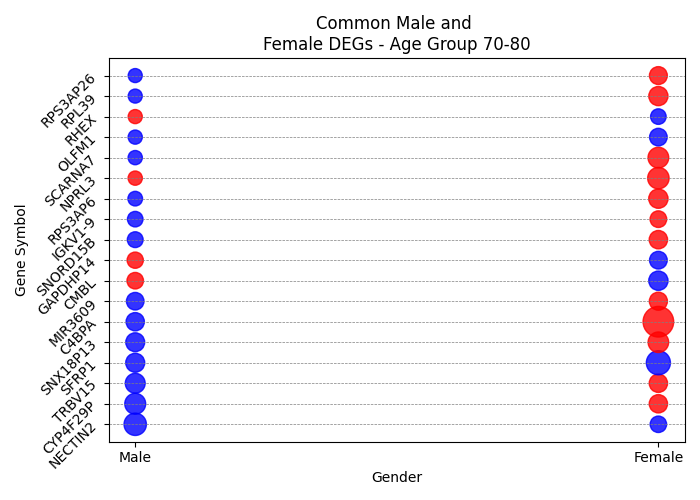
\includegraphics[width=\textwidth]{Chapter-3/bubbleplot_combined_70-80.png}
                            \caption{Κοινά διαφορικά εκφραζόμενα γονίδια ηλικίας 70-80}
                            \label{fig:bubbleplot_combined_70-80}
                        \end{subfigure}
                        \hfill
                        \begin{subfigure}[b]{0.48\textwidth}
                            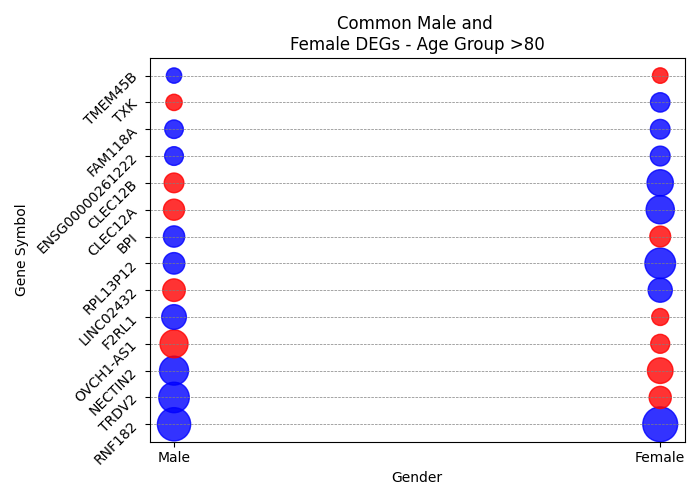
\includegraphics[width=\textwidth]{Chapter-3/bubbleplot_combined_>80.png}
                            \caption{Κοινά διαφορικά εκφραζόμενα γονίδια ηλικίας >80}
                            \label{fig:bubbleplot_combined_>80}
                        \end{subfigure}
                        
                        \caption{Κοινά διαφορικά εκφραζόμενα γονίδια μεταξύ ανδρών και γυναικών}
                        \label{fig:common-genes-across-genders-per-age-group}
                    \end{figure}
                \newpage
                \par    
                    Με μια σύντομη αναζήτηση των, μεταξύ των δύο φύλων κοινών, γονιδίων στη βάση Gene4PD(\emph{\cite{Li2021Gene4PD:Disease}}), μιας βάσης δεδομένων στο διαδίκτυο για την αναζήτηση γενετικών πληροφοριών σχετικά με τη νόσο του Πάρκινσον, ανέκυψαν αποτελέσματα τα οποία συνοψίζονται στον πίνακα~\ref{tab:gene4pd-known-genes}. Υπάρχει μια μίξη μεταξύ γονιδίων που συμμετέχουν σε νευροβιολογικές διεργασίες αλλά και σε διεργασίες σχετικές με το ανοσοποιητικό σύστημα. 
                    \begin{table}[ht]
                        \centering
                        \scriptsize
                        % \setlength{\tabcolsep}{5pt}
                        % \renewcommand{\arraystretch}{1.4}
                        \begin{tabular}{ccc}
                            \textbf{Ηλικιακή ομάδα} & \textbf{Γονίδιο} & \textbf{Εμπλοκή σε βιολογική λειτουργία}\\
                            \midrule
                             \multirow{2}{*}{30-50} & IF27\tablefootnote{http://genemed.tech/gene4pd/geneDetail/main?gene\_symbol=IFI27} & 
                             \parbox{9cm}{Ανοσοποιητικό - Ρύθμιση Ουβικουιτίνης (\emph{\cite{Xue2016ISG12aPathway}}), μονοπάτι σηματοδότησης Jak/STAT (\emph{\cite{Chen2017ISG12aApoptosis}, \cite{Lashgari2021TheDisease}})}
                             \\
                             & MYOM2\tablefootnote{http://genemed.tech/gene4pd/geneDetail/main?gene\_symbol=MYOM2} &
                             \parbox{9cm}{Μυοσκελετικό - \cite{QuickGO::TermGO:0006936} Οντολογία σχετίζεται με μυϊκή συστολή.}
                             \\
                             \midrule
                             50-70 & - & - \\
                             \midrule
                             \multirow{5}{*}{70-80} & RPL39\tablefootnote{http://genemed.tech/gene4pd/geneDetail/main?gene\_symbol=RPL39} & \parbox{9cm}{Ριβοσωμική πρωτεΐνη} \\
                             & NECTIN2\tablefootnote{http://genemed.tech/gene4pd/geneDetail/main?gene\_symbol=NECTIN2} & 
                             \parbox{9cm}{Υποδοχέας ιού του απλού έρπητα (\emph{\cite{Martinez2001StructuralEntry}})}\\
                             & OLFM1\tablefootnote{http://genemed.tech/gene4pd/geneDetail/main?gene\_symbol=OLFM1} & 
                             \parbox{9cm}{Νευρικό σύστημα - (\emph{\cite{Sultana2011OlfactomedinProteins}, \cite{Kelly2019GeneDisease}})}\\
                             & CMBL\tablefootnote{http://genemed.tech/gene4pd/geneDetail/main?gene\_symbol=CMBL} & 
                             \parbox{9cm}{Ένζυμο υδρόλυσης}\\
                             & SFRP1\tablefootnote{http://genemed.tech/gene4pd/geneDetail/main?gene\_symbol=SFRP1} & 
                             \parbox{9cm}{Νευρικό σύστημα - (\emph{\cite{Kele2012SFRP1Cells}})}\\
                             \midrule
                             \multirow{2}{*}{>80} & TXK\tablefootnote{http://genemed.tech/gene4pd/geneDetail/main?gene\_symbol=TXK} & 
                             \parbox{9cm}{Ανοσοποιητικό - (\emph{\cite{Kashiwakura1999TxkLymphocytes}})}\\
                             & NECTIN2 & -"-\\
                        \end{tabular}
                        \caption{Διαφορικά εκφραζόμενα γονίδια σχετικά με την νόσο του Πάρκινσον σύμφωνα με τη βάση δεδομένων Gene4PD}
                        \label{tab:gene4pd-known-genes}
                    \end{table}                    
        \newpage
    \section{Κατηγοριοποίηση δειγμάτων μέσω Μηχανικής Μάθησης}
        \par
            Με την χρήση των δεδομένων της διαφορικής ανάλυσης γονιδιακής έκφρασης εκπαιδεύτηκαν τέσσερις διαφορετικοί κατηγοριοποιητές εποπτευόμενης μάθησης. Χρησιμοποιήθηκαν οι αλγόριθμοι λογιστικής παλινδρόμησης, SVM\nomenclature{SVM}{Support Vector Machines}, Random Forest και XGBoost. Πρόκειται για αλγόριθμους που χρησιμοποιούνται, μεταξύ άλλων, στον τομέα της βιοπληροφορικής.
        \par
            Η εφαρμογή της κατηγοριοποίησης πραγματοποιήθηκε σε όλα τα στρώματα (\emph{strata}) του συνόλου δεδομένων. Ως αποτελέσματα για την αποτίμηση της επίδοσης του κάθε αλγορίθμου ανά στρώμα, χρησιμοποιήθηκαν καθιερωμένες μετρικές όπως ROC-AUC\nomenclature{ROC-AUC}{Receiver Operating Characteristic}\nomenclature{AUC}{Area Under the Curve}, PR-AUC\nomenclature{PR}{Precission Recall} καθώς και η ευαισθησία και η ειδικότητα της κατηγοριοποίησης κατά την εκτέλεση. Η εκπαίδευση λειτούργησε με τη χρήση ενός εύρους παραμέτρων (\emph{Hyperparameters}) μέσω των οποίων ο κατηγοριοποιητής της κάθε μεθόδου δοκιμάζει και αποφασίζει τον βέλτιστο συνδυασμό παραμέτρων μετά από δεκαπλάσια διασταυρούμενη επικύρωση (\emph{10-fold Cross Validation}). Ο έτσι παραμετροποιημένος βέλτιστος κατηγοριοποιητής εκπαιδεύεται και μετέπειτα δοκιμάζεται σε κατηγοριοποίηση επί του αντίστοιχου συνόλου. Ανεξάρτητα της εύρεσης του καλύτερου δυνατού κατηγοριοποιητή ανά αλγόριθμο, η δεκαπλάσια διασταυρούμενη επικύρωση λαμβάνει χώρα και ξεχωριστά από την παραπάνω διαδικασία, ως μέτρο παρουσίασης της γενικής επίδωσης του κάθε μοντέλου κατηγοριοποίησης.
            \begin{figure}[h]
                \centering
                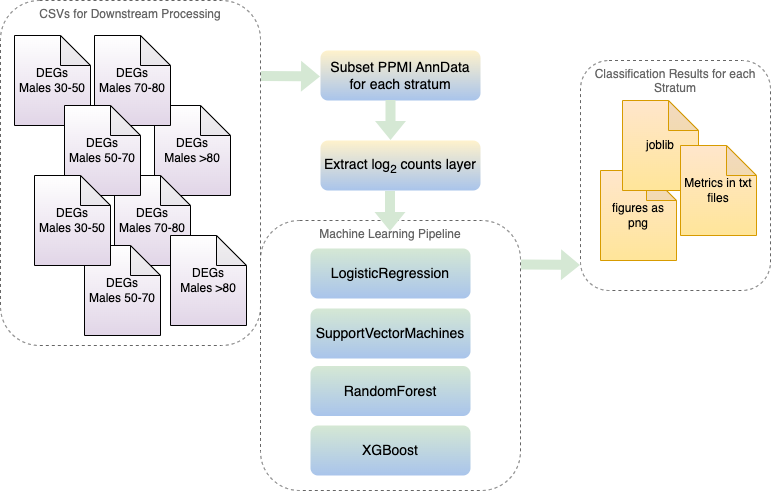
\includegraphics[width=0.7\textwidth]{ML/msci-big-pic-ML-blocks.png}
                \caption{Pipeline για την κατηγοριοποίηση δειγμάτων με χρήση μηχανικής μάθησης}
                \label{fig:msci-big-pic-ML-blocks}
            \end{figure}
        \par
            Τα σύνολα εκπαίδευσης και εκτέλεσης είναι διαφορετικά, με το σύνολο εκπαίδευσης να επιλέγεται στο 80\% επί του συνόλου δεδομένων ανά στρώμα, όπως και επίσης δείγματα από τα ίδια άτομα δεν βρίσκονται και στα δυο σύνολα, κάτι που θα είχε ως αποτέλεσμα το φαινόμενο του Feature Leakage (\emph{\cite{Oosterhuis2024LocalPredictions}}) και θα παραποιούσε σημαντικά τις μετρικές καθώς και την έκβαση της κατηγοριοποίησης. Για την επίτευξη του διαχωρισμού έγινε χρήση της κλάσης GroupShuffleSplit στην Python, από το πακέτο scikit (\emph{\cite{Buitinck2013APIProject}}). 
        \par
            Παρότι τα δείγματα των νοσούντων είναι σε όλα τα στρώματα περίπου διπλάσια των υγιών, η ανισορροπία (\emph{Class imbalance}) δεν είναι αρκετά υψηλή ώστε να δημιουργήσει σημαντικά προβλήματα, όπως την προνομιακή κατηγοριοποίηση με γνώμονα την πολυπληθέστερη ομάδα (\emph{εικόνα~\ref{fig:ppmi-visual-bar-class-imb}}). Για το λόγο αυτό και επίσης για την αποφυγή υπέρ-αισιόδοξων αποτελεσμάτων κατηγοριοποίησης, δεν επιδιώχθηκε η χρήση μεθόδων όπως π.χ.  SMOTE\nomenclature{SMOTE}{Synthetic Minority Oversampling Technique}.

            \begin{figure}[H]
                \centering
                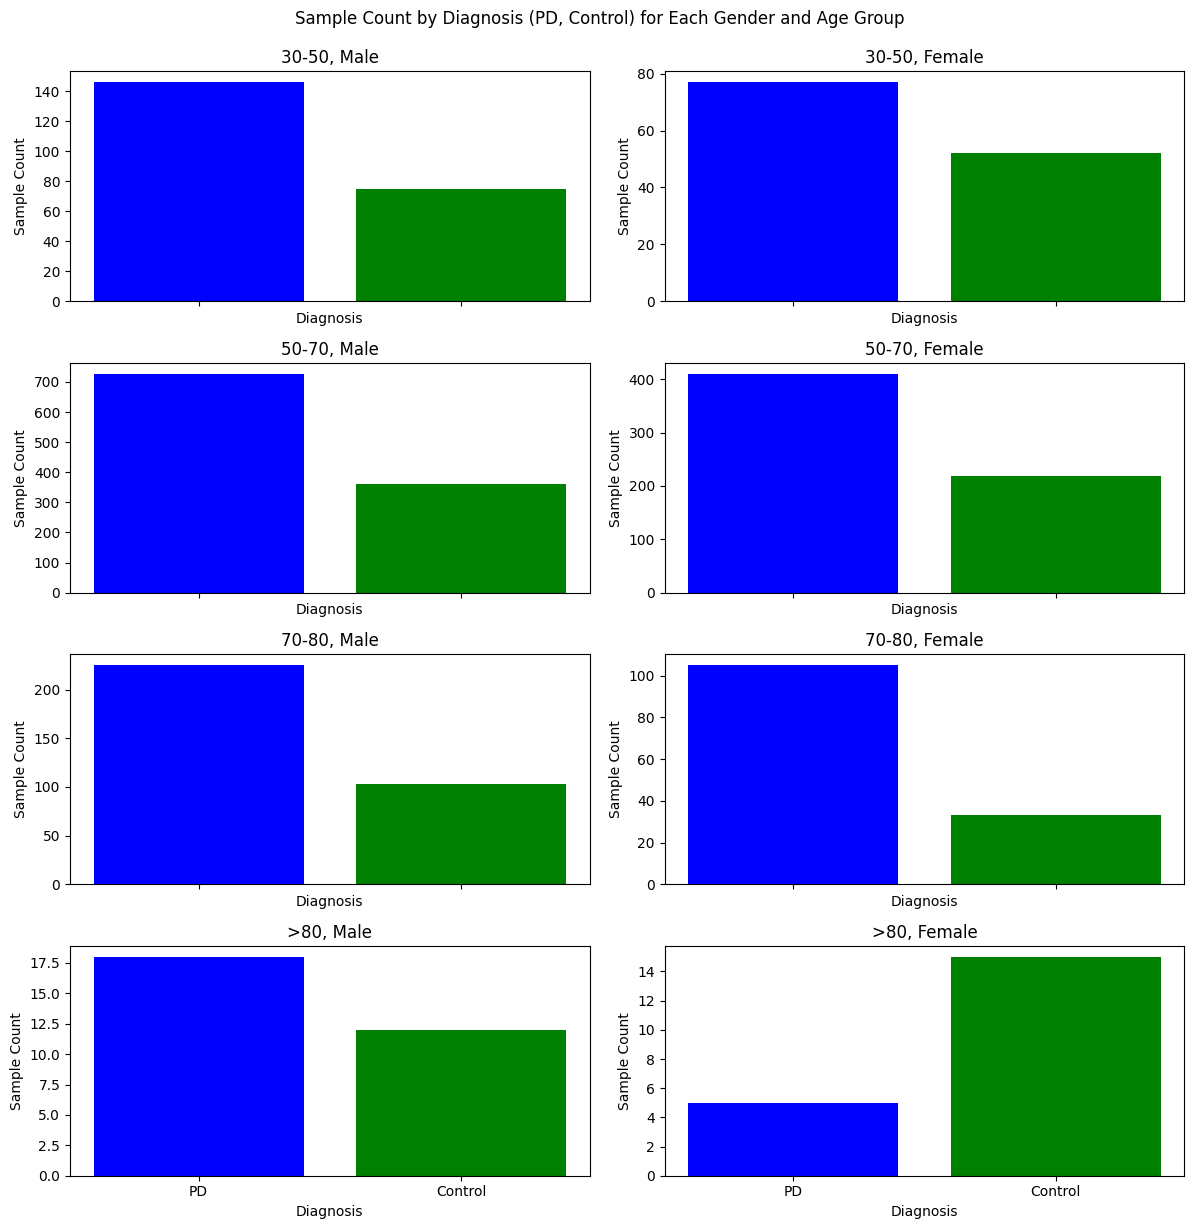
\includegraphics[width=0.7\textwidth]{ML/ppmi-visual-bar-class-imb.png}
                \caption[Απεικόνιση ανισορροπίας μεταξύ των ομάδων της μελέτης] {Στις ομάδες ανδρών 30-50, 50-70 και 70-80 παρατηρείται ανισορροπία κατά περίπου το διπλάσιο της ομάδας ελέγχου. Στις ομάδες γυναικών 50-70 επίσης, ενώ στην ηλικιακή ομάδα 70-80 περίπου το τριπλάσιο. Η ομάδα γυναικών στις ηλικίες άνω των 80 δείχνει σχεδόν τριπλάσια δείγματα ελέγχου αντί νοσούντων.}
                \label{fig:ppmi-visual-bar-class-imb}
            \end{figure}
        \subsection{Επιδόσεις κατηγοριοποίησης}
                Οι επιδόσεις της κατηγοριοποίησης ποικίλουν ανά στρώμα, δηλαδή τον συνδυασμό φύλου και ηλικιακής ομάδας. Η πιο αντιπροσωπευτική ομάδα από άποψη του πλήθους των διαθέσιμων δειγμάτων παρουσιάζεται παρακάτω. Τα αποτελέσματα των λοιπών ομάδων παρατίθενται στο παράρτημα της εργασίας.
            \par
                Αρχικά, παρατηρούνται οι μετρικές της δεκαπλάσιας διασταυρούμενης επικύρωσης των διαφόρων αλγορίθμων κατηγοριοποίησης στην εικόνα~\ref{fig:ml-algorithms-k-fold-validation}. Απεικονίζονται οι καμπύλες ROC-AUC ως παράσταση των αληθώς θετικών προβλέψεων έναντι των ψευδώς θετικών και η PR-AUC ως παράσταση της ακρίβειας και της ευαισθησίας ή ανάκλησης. Τα αποτελέσματα όλων των κατηγοριοποιητών για το γυναικείο φύλο κυμαίνονται μεταξύ της χαμηλότερης τιμής 0,72 και της υψηλότερης 0,77 για τη μετρική ROC-AUC, όπου η χαμηλότερη μέση τιμή αποδίδεται από τον αλγόριθμο XGBoost και η υψηλότερη από τον αλγόριθμο της λογιστικής παλινδρόμησης. Αντίστοιχα, η μετρική PR-AUC βρίσκεται μεταξύ χαμηλού 0,81 από τους αλγόριθμους Random Forest και XGBoost και 0,83 από την λογιστική παλινδρόμηση και SVM. Στους άνδρες οι υψηλότερες μέσες τιμές για ROC-AUC και PR-AUC αποδίδονται από τον αλγόριθμο XGBoost με 0,73 και 0,84 αντίστοιχα. Η χαμηλότερη επίδοση αποδίδεται από την λογιστική παλινδρόμηση με 0,55 για ROC-AUC και 0,70 για PR-AUC. Η χαμηλή ROC-AUC καθιστά την επίδοση της λογιστικής παλινδρόμησης ελαφρώς καλύτερη από ένα μοντέλο τυχαίων προβλέψεων, λόγω της εγγύτητας στο κατώφλι αξιολόγησης των 50\%. Η βελτιωμένη επίδοση του XGBoost πιθανώς μπορεί να αποδοθεί στο μεγαλύτερο πλήθος δειγμάτων και με αυτό, μεγαλύτερο πλήθος δεδομένων μάθησης σε σύγκριση με το σύνολο των γυναικών, παρόλο που η ανισορροπία και στις δυο περιπτώσεις κυμαίνεται σε αναλογία 2 προς 1.      
                \newpage
                \begin{figure}[H]
                    \centering
                    \begin{subfigure}[b]{0.48\textwidth}
                        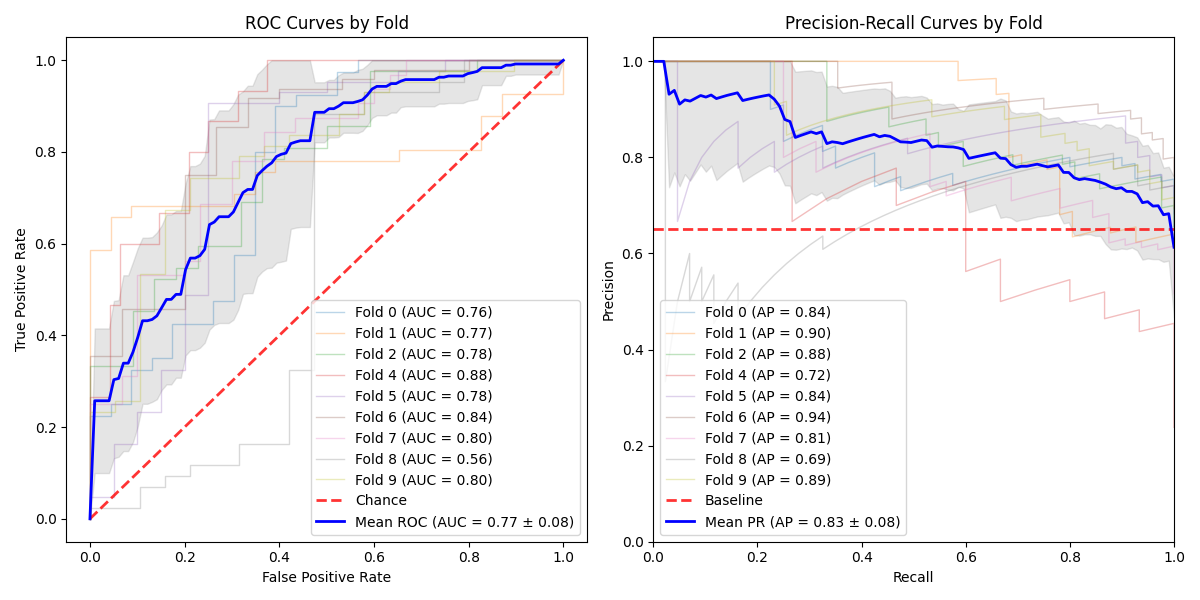
\includegraphics[width=\textwidth]{ML/CV/stratified_Female_50-70_LR_useSMOTE_False_k_fold_validation.png}
                        \caption{Γυναίκες: Λογιστική παλινδρόμηση}
                        \label{stratified_Female_50-70_LR_useSMOTE_False_k_fold_validation}
                    \end{subfigure}
                    \hfill
                    \begin{subfigure}[b]{0.48\textwidth}
                        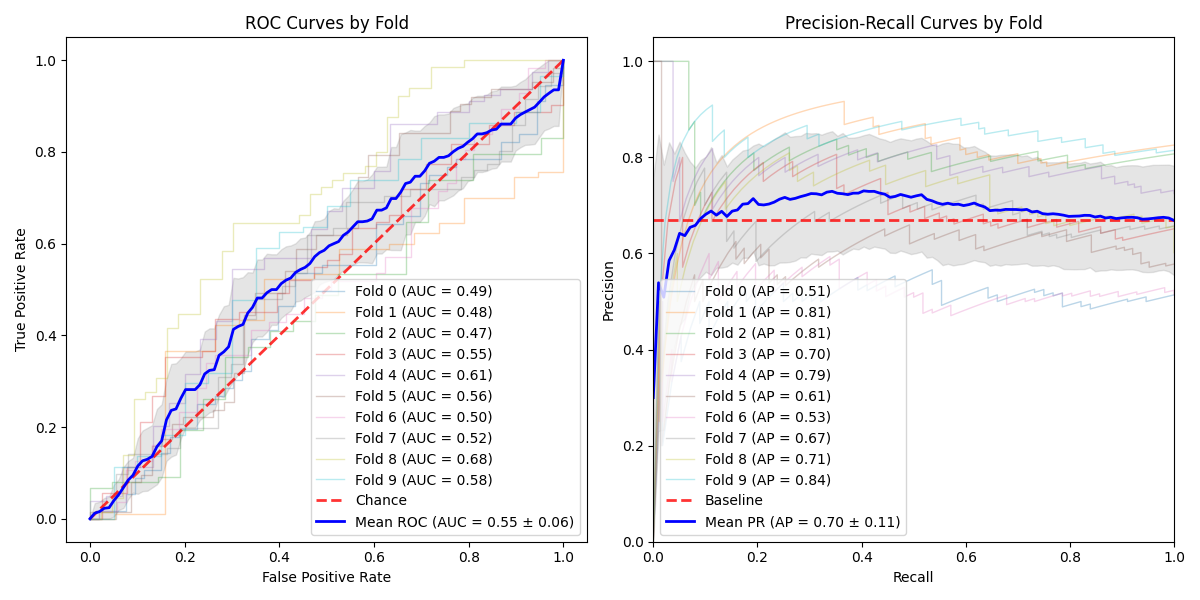
\includegraphics[width=\textwidth]{ML/CV/stratified_Male_50-70_LR_useSMOTE_False_k_fold_validation.png}
                        \caption{Άνδρες: Λογιστική παλινδρόμηση}
                        \label{stratified_Male_50-70_LR_useSMOTE_False_k_fold_validation}
                    \end{subfigure}
                    \vspace{0.5cm}
                    \begin{subfigure}[b]{0.48\textwidth}
                        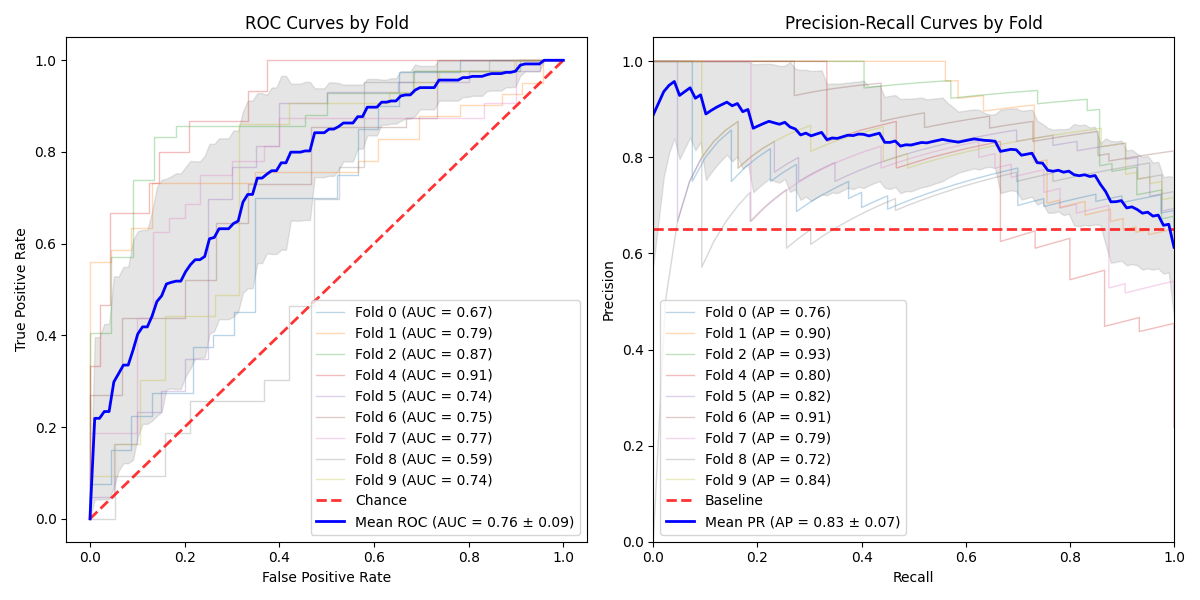
\includegraphics[width=\textwidth]{ML/CV/stratified_Female_50-70_SVM_useSMOTE_False_k_fold_validation.png}
                        \caption{Γυναίκες: Support Vector Machine}
                        \label{stratified_Female_50-70_SVM_useSMOTE_False_k_fold_validation}
                    \end{subfigure}
                    \hfill
                    \begin{subfigure}[b]{0.48\textwidth}
                        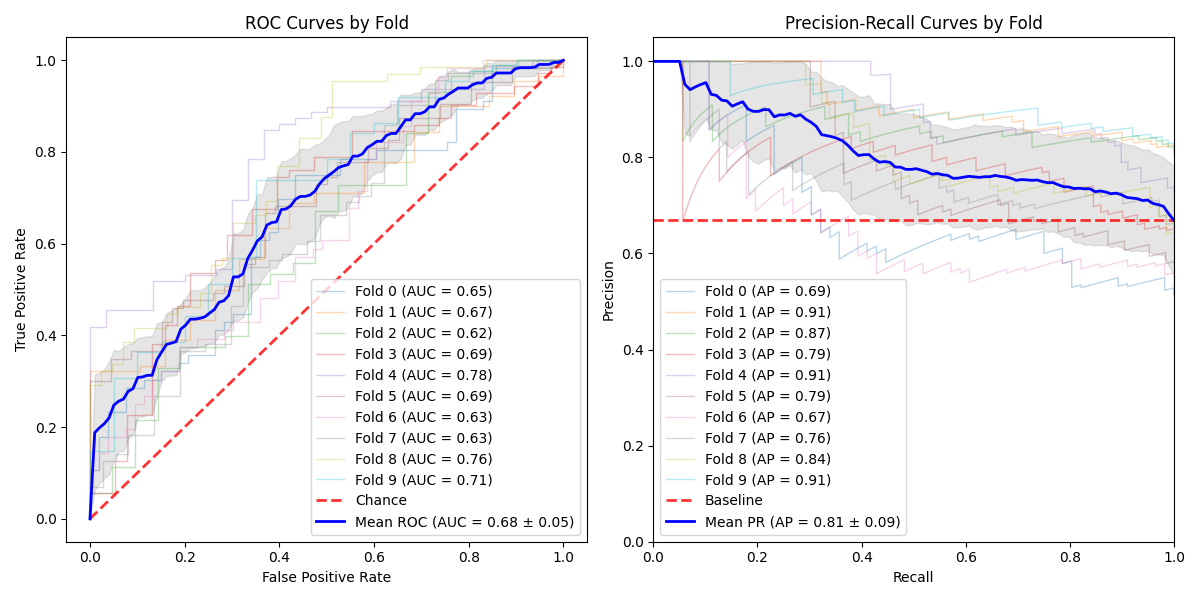
\includegraphics[width=\textwidth]{ML/CV/stratified_Male_50-70_SVM_useSMOTE_False_k_fold_validation.png}
                        \caption{Άνδρες: Support Vector Machine}
                        \label{stratified_Male_50-70_SVM_useSMOTE_False_k_fold_validation}
                    \end{subfigure}
                    \vspace{0.5cm}
                    \begin{subfigure}[b]{0.48\textwidth}
                        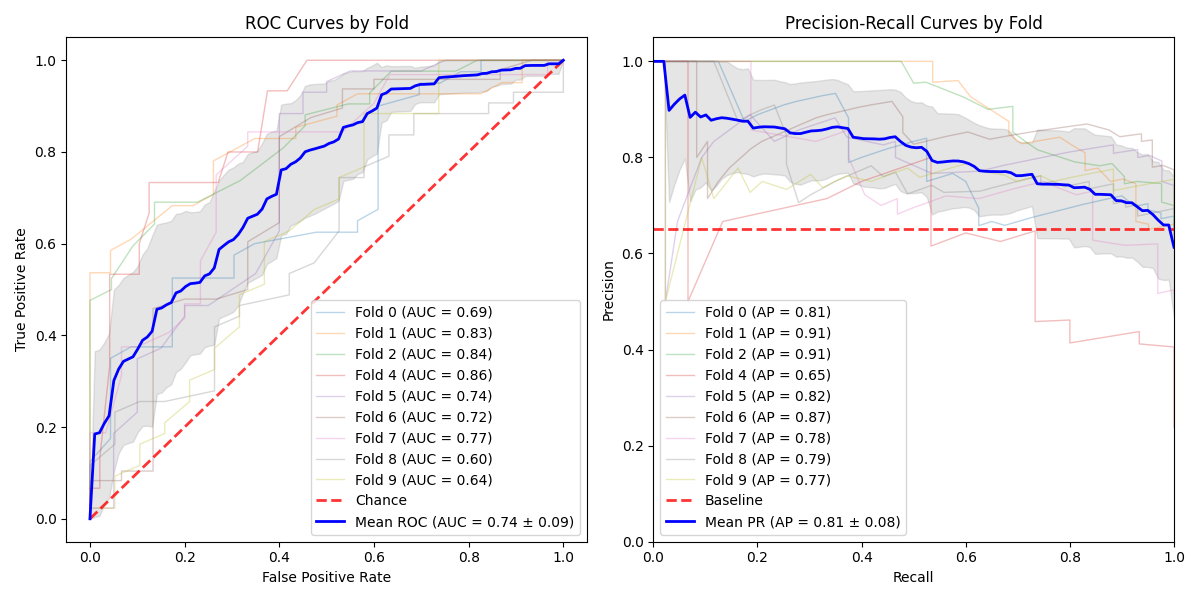
\includegraphics[width=\textwidth]{ML/CV/stratified_Female_50-70_RF_useSMOTE_False_k_fold_validation.png}
                        \caption{Γυναίκες: Random Forest}
                        \label{stratified_Female_50-70_RF_useSMOTE_False_k_fold_validation}
                    \end{subfigure}
                    \hfill
                    \begin{subfigure}[b]{0.48\textwidth}
                        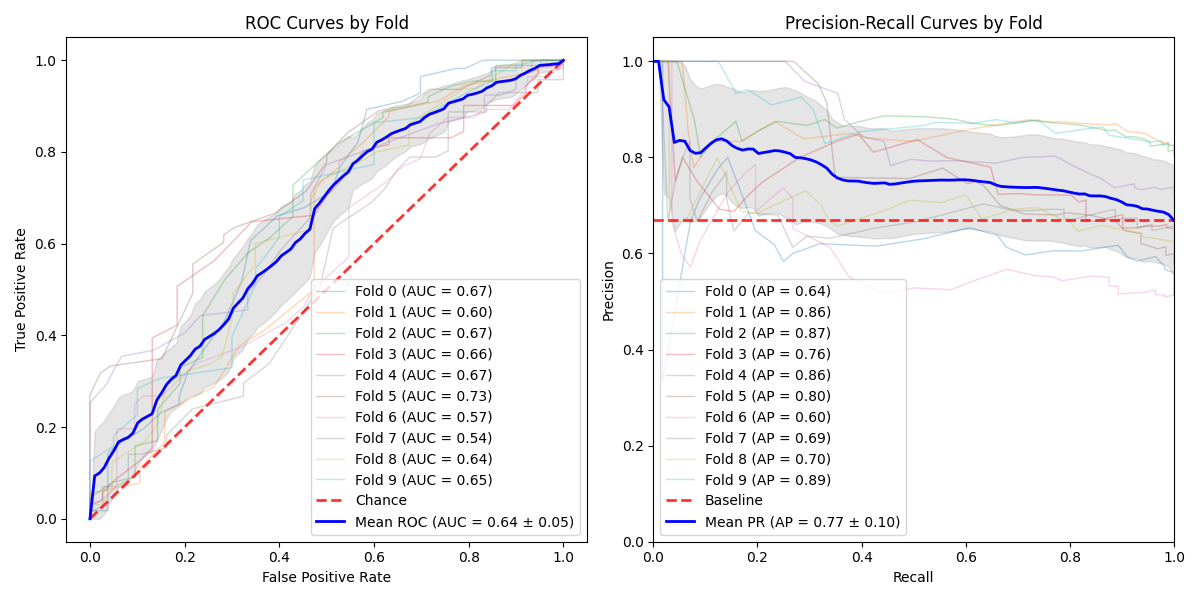
\includegraphics[width=\textwidth]{ML/CV/stratified_Male_50-70_RF_useSMOTE_False_k_fold_validation.png}
                        \caption{Άνδρες: Random Forest}
                        \label{stratified_Male_50-70_RF_useSMOTE_False_k_fold_validation}
                    \end{subfigure}
                    \vspace{0.5cm}
                    \begin{subfigure}[b]{0.48\textwidth}
                        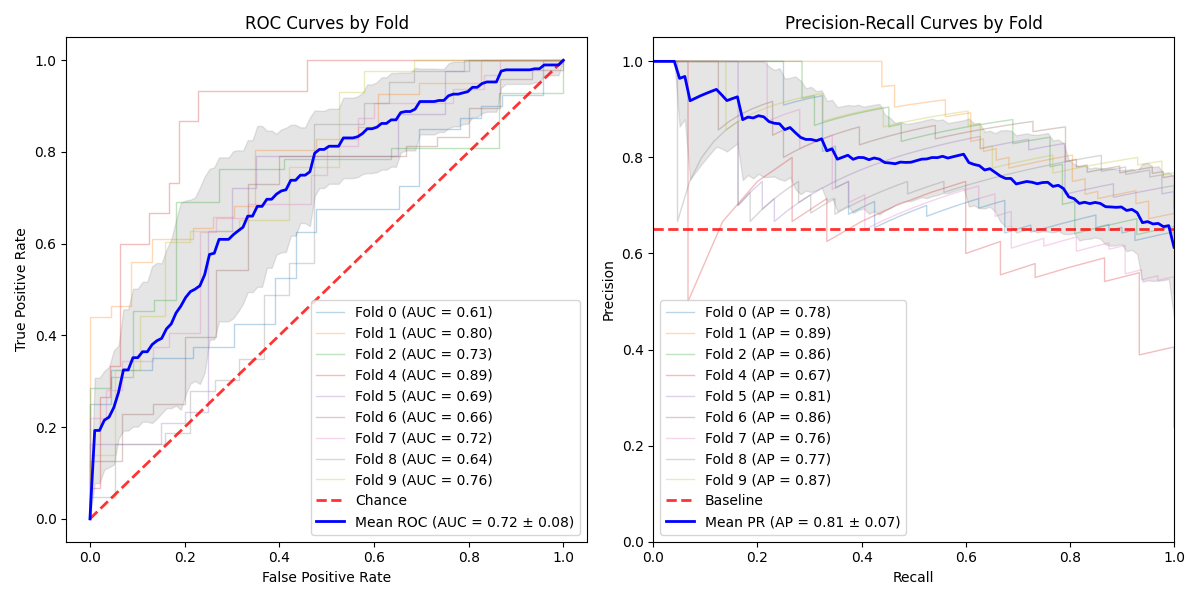
\includegraphics[width=\textwidth]{ML/CV/stratified_Female_50-70_XGBOOST_useSMOTE_False_k_fold_validation.png}
                        \caption{Γυναίκες: XGBoost}
                        \label{stratified_Female_50-70_XGBOOST_useSMOTE_False_k_fold_validation}
                    \end{subfigure}
                    \hfill
                    \begin{subfigure}[b]{0.48\textwidth}
                        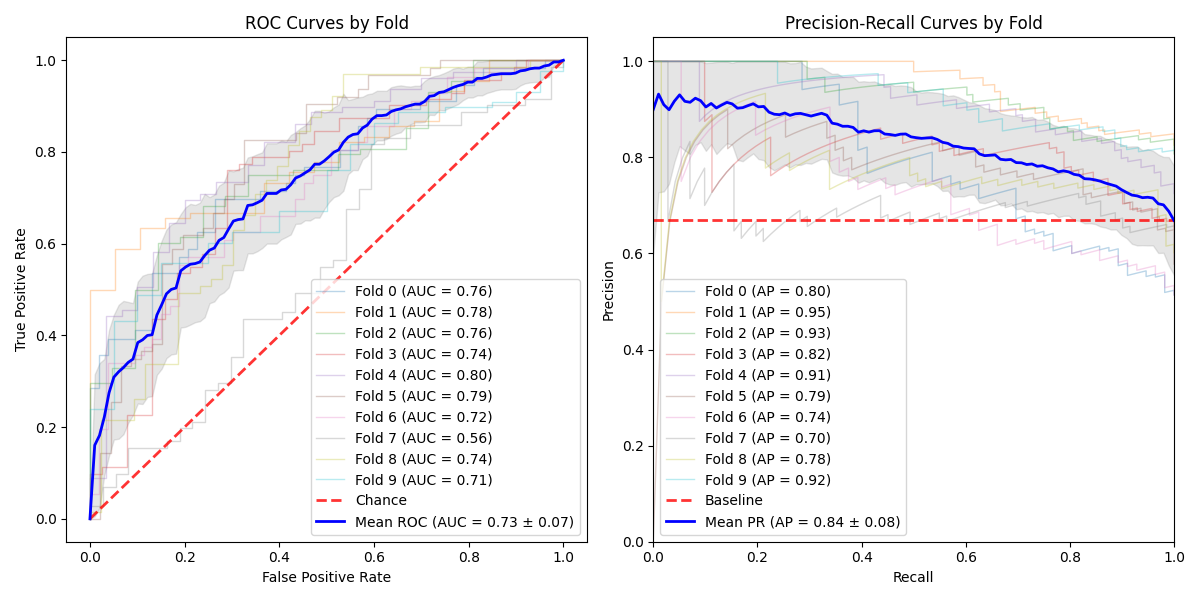
\includegraphics[width=\textwidth]{ML/CV/stratified_Male_50-70_XGBOOST_useSMOTE_False_k_fold_validation.png}
                        \caption{Άνδρες: XGBoost}
                        \label{stratified_Male_50-70_XGBOOST_useSMOTE_False_k_fold_validation}
                    \end{subfigure}
                    \vspace{-0.5cm}
                    \caption{Αποτελέσματα δεκαπλάσιας διασταυρούμενης επικύρωσης}
                    \label{fig:ml-algorithms-k-fold-validation}               
                \end{figure}
            \newpage
                Ο πίνακας~\ref{tab:ml-classification-metrics-detailed} περιέχει μετρικές όπως την ακρίβεια (\emph{Precision}), την ανάκληση ή ευαισθησία (\emph{Recall}) για κάθε κλάση ταξινόμησης (\emph{HC\nomenclature{HC}{Healthy Control}=ομάδα υγειών/ελέγχου, PD=ομάδα νοσού Πάρκινσον}) και τις τιμές ROC-AUC και PR-AUC. Στις στήλες είναι ο αλγόριθμος κατηγοριοποίησης (\emph{LR=Λογιστική Παλινδρόμηση, SVM=Support Vector Machine, RF=Random Forest, XGB=XGBoost}) κάτω από τον οποίο καταγράφονται τα αποτελέσματα για άνδρες και γυναίκες (\emph{M=Male, F=Female}). 
            \par
                Η τιμή της ακρίβειας ορίζεται από το λόγο των αληθώς θετικών προς το σύνολο των θετικών προβλέψεων και καταγράφει την επίδοση του κατηγοριοποιητή να διακρίνει περιπτώσεις θετικών δειγμάτων ως προς την κλάση αναφοράς, που όπως απεικονίζεται στον πίνακα~\ref{tab:ml-classification-metrics-detailed} η τιμή υπολογίζεται τόσο για την ομάδα νοσούντων όσο και για την ομάδα ελέγχου. Η τιμή της ευαισθησίας ή ανάκλησης αφορά, όπως και η ακρίβεια, κάθε κλάση στον παρακάτω πίνακα και υπολογίζεται ως λόγος αληθώς θετικών προβλέψεων προς το σύνολο των προβλέψεων.

                \begin{table}[H]
                    \centering
                    \setlength{\tabcolsep}{4pt} 
                    \begin{tabular}{lccccccccc}
                        \multirow{2}{*}{} & \multirow{2}{*}{} & \multicolumn{2}{c}{\textbf{LR}} & \multicolumn{2}{c}{\textbf{SVM}} & \multicolumn{2}{c}{\textbf{RF}} & \multicolumn{2}{c}{\textbf{XGB}} \\
                        & & M & F & M & F & M & F & M & F \\
                        \midrule
                        \multirow{2}{*}{Precision} 
                            & HC & 0,37 & 0,56 & 0,52 & 0,68 & 0,50 & \textbf{0,80} & 0,59 & 0,59 \\
                            & PD & \textbf{0,70} & \textbf{0,72} & \textbf{0,75} & 0,69 & \textbf{0,70} & 0,65 & \textbf{0,74} & 0,68 \\
                        \multirow{2}{*}{Recall}
                            & HC & 0,38 & \textbf{0,71} & 0,45 & 0,54 & 0,13 & 0,36 & 0,33 & 0,57 \\
                            & PD & \textbf{0,70} & 0,58 & \textbf{0,80} & \textbf{0,81} & \textbf{0,94} & \textbf{0,93} & \textbf{0,89} & \textbf{0,70} \\
                        \midrule
                        ROC-AUC & & \multicolumn{2}{c}{0,582} & \multicolumn{2}{c}{0,707} & \multicolumn{2}{c}{0,636} & \multicolumn{2}{c}{0,694} \\
                        PR-AUC & & \multicolumn{2}{c}{0,739} & \multicolumn{2}{c}{0,747} & \multicolumn{2}{c}{0,796} & \multicolumn{2}{c}{0,790} \\
                    \end{tabular}
                    \caption{Αναλυτικές μετρικές επίδοσης κατηγοριοποίησης}
                    \label{tab:ml-classification-metrics-detailed}
                \end{table}
                \par
                    Η ευαισθησία του μοντέλου Random Forest βρίσκεται σε εξαιρετικά υψηλά επίπεδα και για τα δύο φύλα. Υψηλές τιμές ευαισθησίας παρουσιάζονται επίσης από το μοντέλο SVM. Ο αλγόριθμος XGBoost παρουσιάζει υψηλό σκορ ανάκλησης για άνδρες και μειωμένο για τις γυναίκες. Αντίστοιχα, στη λογιστική παλινδρόμηση για τους άνδρες η ευαισθησία βρίσκεται σε ένα ικανοποιητικό  επίπεδο των 70\%. Με αυτές τις τιμές ευαισθησίας, τα προαναφερόμενα μοντέλα κατηγοριοποίησης παρουσιάζουν σχετικά ικανοποιητική επίδοση σχετικά με την ανίχνευση θετικών ως προς την νόσο του Πάρκινσον. Ως προς την ακρίβεια, η λογιστική παλινδρόμηση παρουσιάζει τιμές $\geq70\%$ και στα δύο φύλα. Η ακρίβεια στους αλγόριθμους Random Forest και XGBoost βρίσκεται για τους άνδρες στο 70\% και 74\% αντίστοιχα. Η υψηλότερη τιμή ακρίβειας ως προς την ομάδα ελέγχου αποδίδεται από το μοντέλο Random Forest με 80\% για τις γυναίκες.
                \par
                    Οι καμπύλες ROC-AUC, PR-AUC και η αντίστοιχη μήτρα σύγχυσης παρουσιάζονται στην εικόνα~\ref{fig:predictions-genders-50-70-all-classifiers}.                
                \begin{figure}[H]
                    \centering
                    \begin{subfigure}[b]{0.48\textwidth}
                        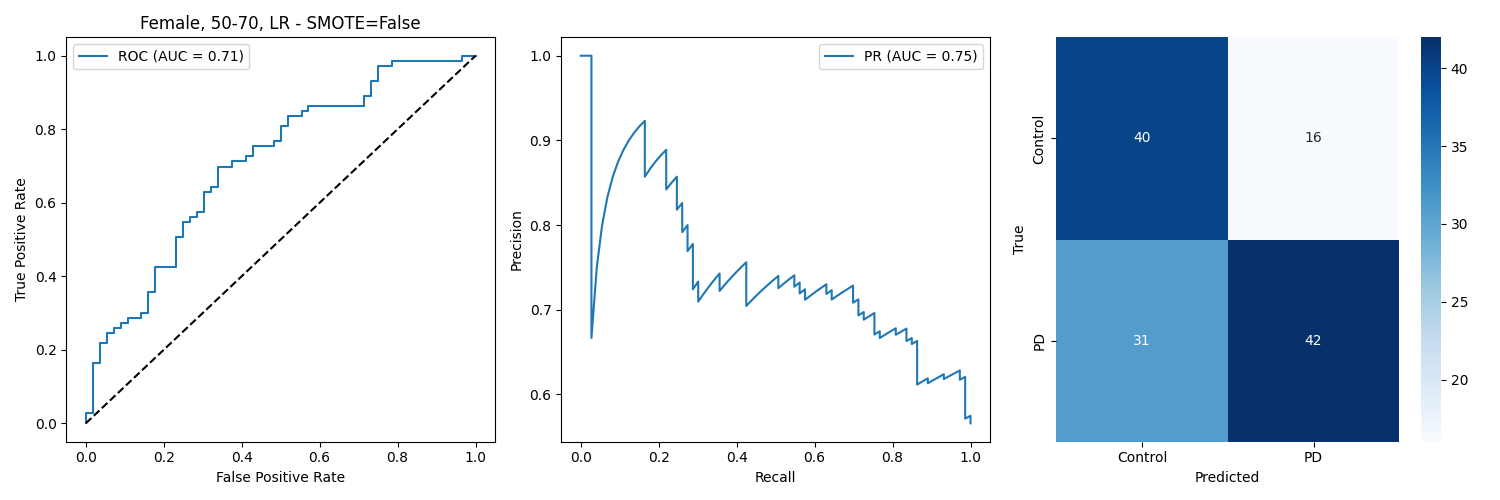
\includegraphics[width=\textwidth]{ML/Predict/DEG/AUC/results_stratified_Female_50-70_LR_useSMOTE_False.png}
                        \caption{Γυναίκες: Λογιστική παλινδρόμηση}
                        \label{fig:results_stratified_Female_50-70_LR_useSMOTE_False}
                    \end{subfigure}
                    \hfill
                    \begin{subfigure}[b]{0.48\textwidth}
                        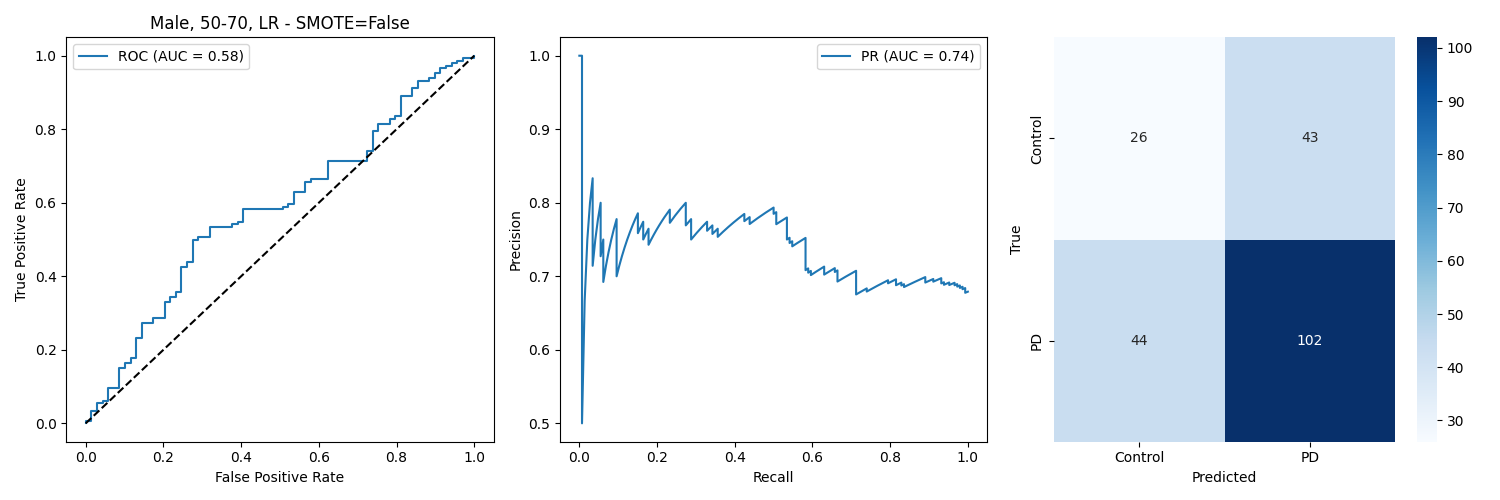
\includegraphics[width=\textwidth]{ML/Predict/DEG/AUC/results_stratified_Male_50-70_LR_useSMOTE_False.png}
                        \caption{Άνδρες: Λογιστική παλινδρόμηση}
                        \label{fig:results_stratified_Male_50-70_LR_useSMOTE_False}
                    \end{subfigure}
                    \vspace{0.5cm}
                    \begin{subfigure}[b]{0.48\textwidth}
                        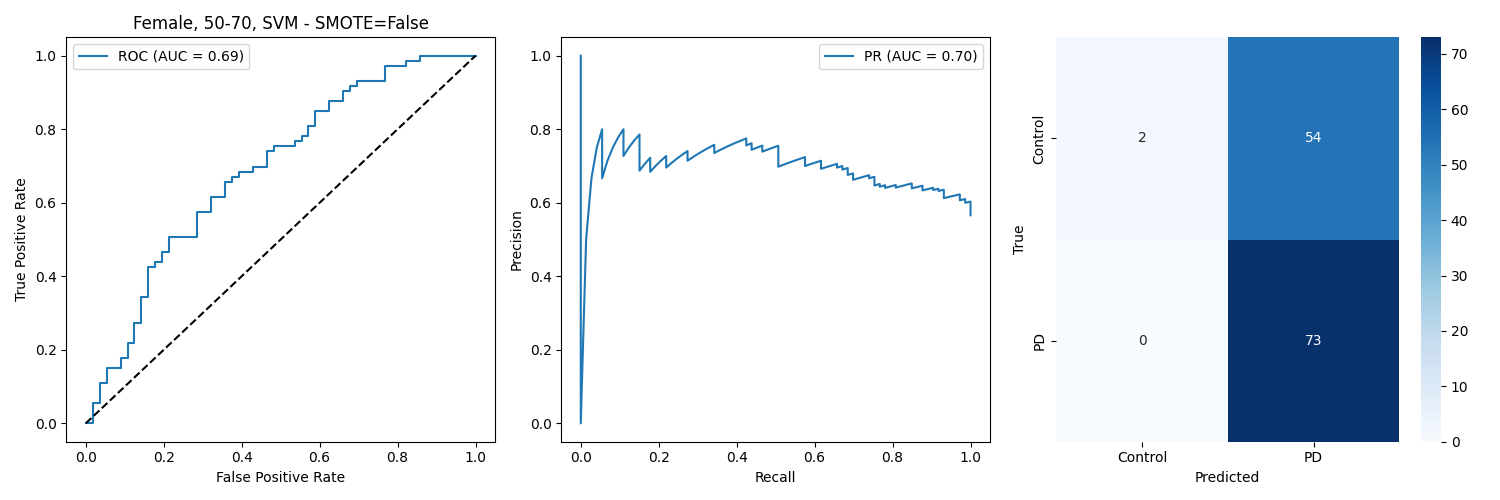
\includegraphics[width=\textwidth]{ML/Predict/DEG/AUC/results_stratified_Female_50-70_SVM_useSMOTE_False.png}
                        \caption{Γυναίκες: SVM}
                        \label{fig:results_stratified_Female_50-70_SVM_useSMOTE_False}
                    \end{subfigure}
                    \hfill
                    \begin{subfigure}[b]{0.48\textwidth}
                        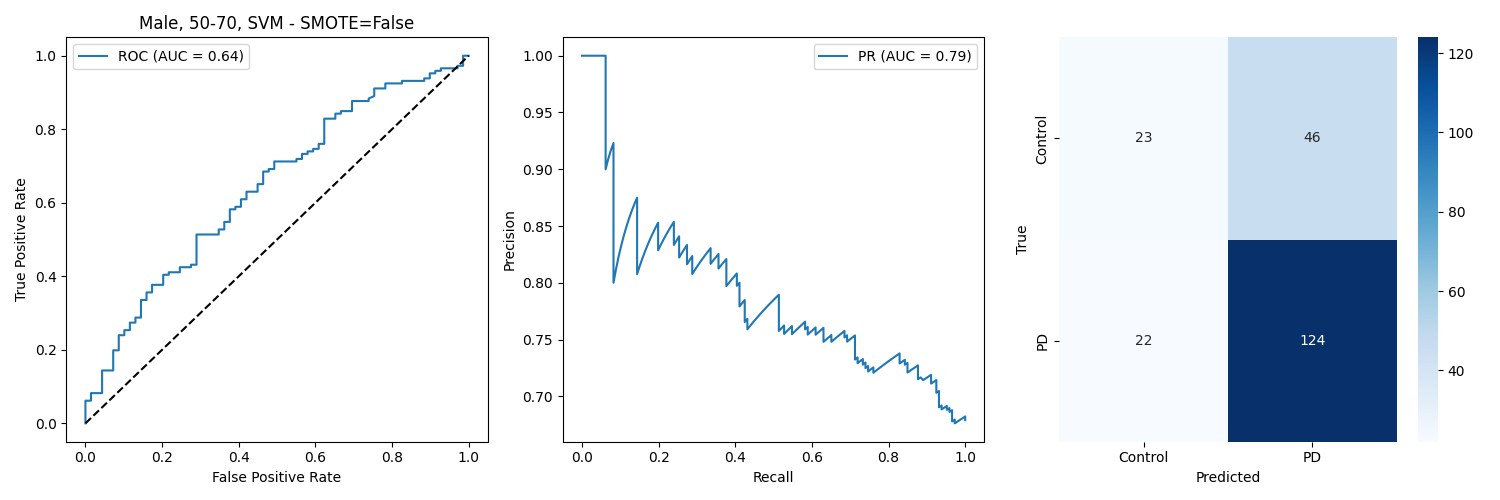
\includegraphics[width=\textwidth]{ML/Predict/DEG/AUC/results_stratified_Male_50-70_SVM_useSMOTE_False.png}
                        \caption{Άνδρες: SVM}
                        \label{fig:results_stratified_Male_50-70_SVM_useSMOTE_False}
                    \end{subfigure}
                    \vspace{0.5cm}
                    \begin{subfigure}[b]{0.48\textwidth}
                        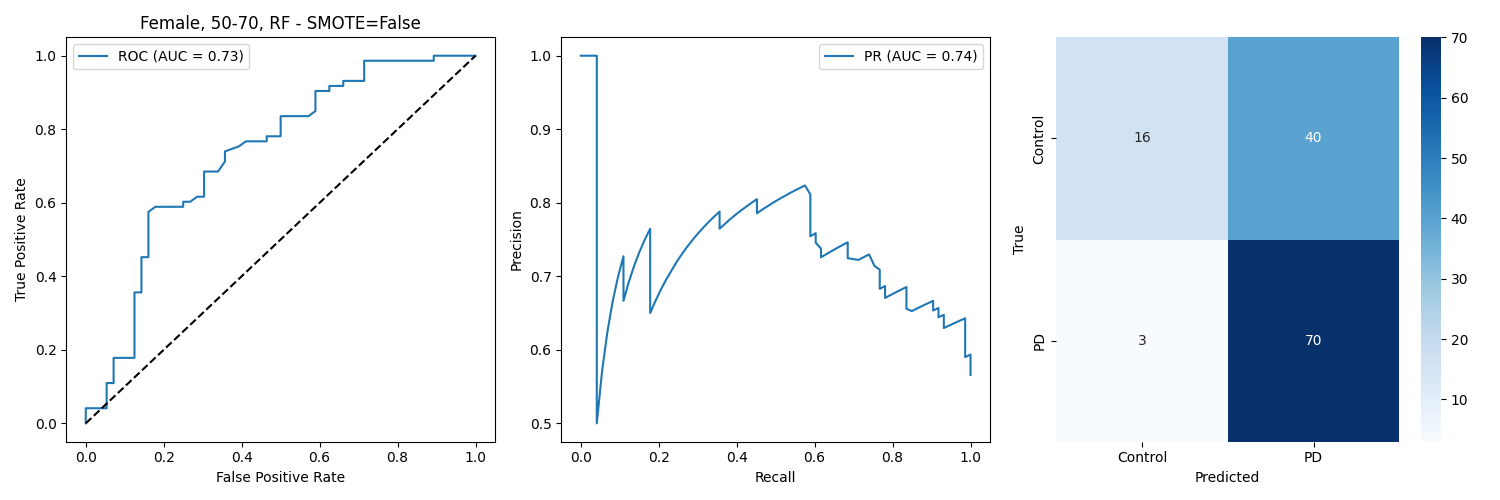
\includegraphics[width=\textwidth]{ML/Predict/DEG/AUC/results_stratified_Female_50-70_RF_useSMOTE_False.png}
                        \caption{Γυναίκες: Random Forest}
                        \label{fig:results_stratified_Female_50-70_RF_useSMOTE_False}
                    \end{subfigure}
                    \hfill
                    \begin{subfigure}[b]{0.48\textwidth}
                        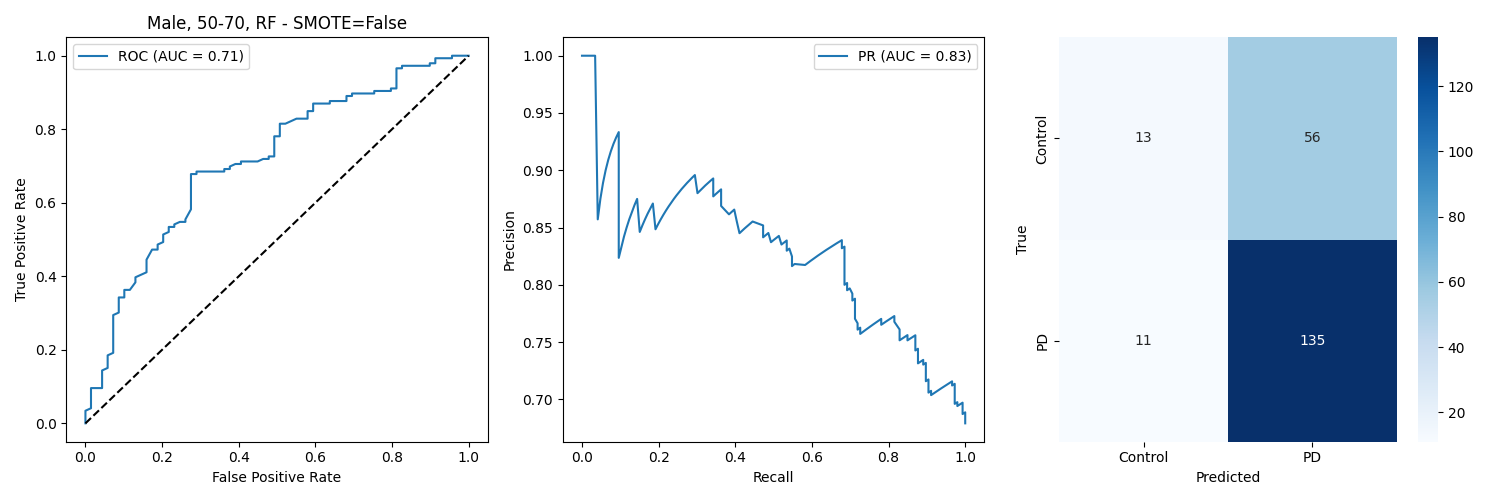
\includegraphics[width=\textwidth]{ML/Predict/DEG/AUC/results_stratified_Male_50-70_RF_useSMOTE_False.png}
                        \caption{Άνδρες: Random Forest}
                        \label{fig:results_stratified_Male_50-70_RF_useSMOTE_False}
                    \end{subfigure}
                    \vspace{0.5cm}
                    \begin{subfigure}[b]{0.48\textwidth}
                        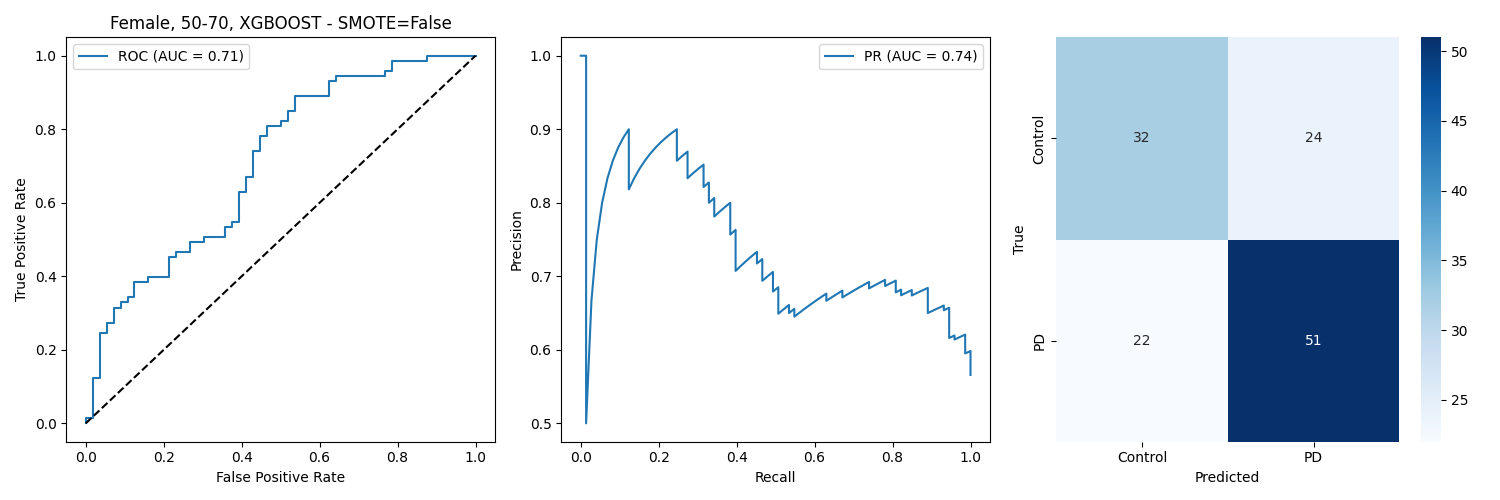
\includegraphics[width=\textwidth]{ML/Predict/DEG/AUC/results_stratified_Female_50-70_XGBOOST_useSMOTE_False.png}
                        \caption{Γυναίκες: XGBoost}
                        \label{fig:results_stratified_Female_50-70_XGBOOST_useSMOTE_False}
                    \end{subfigure}
                    \hfill
                    \begin{subfigure}[b]{0.48\textwidth}
                        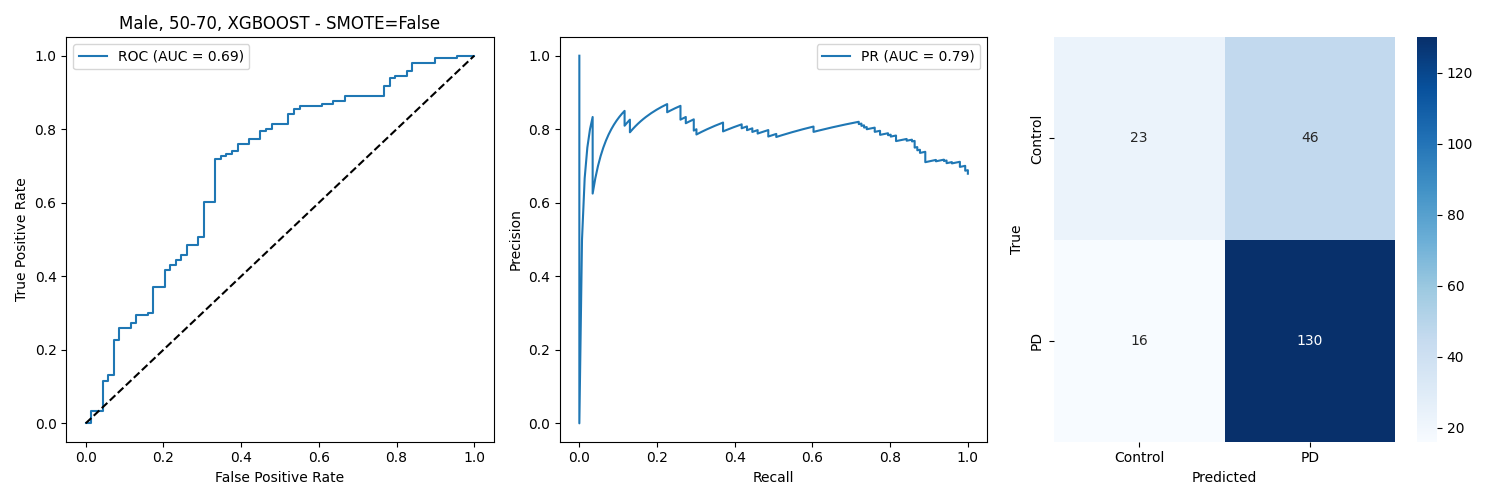
\includegraphics[width=\textwidth]{ML/Predict/DEG/AUC/results_stratified_Male_50-70_XGBOOST_useSMOTE_False.png}
                        \caption{Άνδρες: XGBoost}
                        \label{fig:results_stratified_Male_50-70_XGBOOST_useSMOTE_False}
                    \end{subfigure}
                    \vspace{-0.5cm}
                    \caption{Αποτελέσματα κατηγοριοποίησης ανά φύλο}
                    \label{fig:predictions-genders-50-70-all-classifiers}
                \end{figure}
    \newpage
        \subsection{Αποτίμηση των αποτελεσμάτων της κατηγοριοποίησης}
            Μετά την εκτέλεση της κατηγοριοποίησης προκύπτει το ερώτημα ποια χαρακτηριστικά θεώρησαν τα μοντέλα ταξινόμησης ως παράγοντες διαφοροποίησης μεταξύ των δύο κλάσεων, των υγιών και των νοσούντων ή αλλιώς, ποια είναι τα χαρακτηριστικά που συνέβαλαν περισσότερο ή και λιγότερο, για τη διάκριση των νοσούντων και αντίστοιχα των υγιών.
        \par
            Η ερώτηση μπορεί να απαντηθεί μέσω της εξαγωγής συγκεκριμένων τιμών από τα μοντέλα κατηγοριοποίησης, τα λεγόμενα feature importances που αποδίδουν τιμές σημαντικότητας στα χαρακτηριστικά με βάση των οποίων έγινε η ταξινόμηση. Κάθε μοντέλο κατηγοριοποίησης περιλαμβάνει τρόπους εξαγωγής χαρακτηριστικών, στα οποία αποδίδει και αντίστοιχα σκορ, σύμφωνα με το ρόλο που διαδραμάτισαν στην ταξινόμηση. Τα σκορ που αποδίδονται μπορεί να διαφέρουν αρκετά μεταξύ κατηγοριοποιητών και σε περίπτωση όπου στόχος είναι η σύγκριση των χαρακτηριστικών μεταξύ διάφορων μοντέλων ταξινόμησης, τότε τα σκορ σημαντικότητας πρέπει να κανονικοποιηθούν ώστε να είναι συγκρίσιμα. Επίσης, ο τρόπος με τον οποίο υπολογίζονται τα σημαντικά χαρακτηριστικά της ταξινόμησης μπορεί να διαφέρει από μοντέλο σε μοντέλο και να υπάρχει και μια κλίση σε κατεύθυνση συγκεκριμένων χαρακτηριστικών, η οποία υπόκειται στην αλγοριθμική υλοποίηση, όπως στην περίπτωση του κατηγοριοποιητή Random Forest (\emph{\cite{Strobl2007BiasSolution}}).
        \par
            Η αξιολόγηση της κατηγοριοποίησης μπορεί να επιτευχθεί με ενιαίο και κατανοητό τρόπο με τη χρήση των SHAP\nomenclature{SHAP}{SHapley Additive exPlanation} Values. Πρόκειται για μια μέθοδο η οποία λειτουργεί για κάθε μοντέλο ταξινόμησης με την οποία αποδίδονται σκορ για κάθε χαρακτηριστικό, εξηγώντας πώς αυτό συνέβαλε στην κατηγοριοποίηση. Συγκεκριμένα αποδίδουν το σκορ για το πόσο πολύ ή πόσο λίγο ένα χαρακτηριστικό συνέβαλε στο διαχωρισμό των κλάσεων. Η μέθοδος αυτή χρησιμοποιείται ευρέως σε επιστημονικές έρευνες βιοπληροφορικής όπως \cite{Meral2025Fine-TunedAnalysis} και \cite{FilaliRazzouki2025ExplainingDisease} με στόχο την απάντηση ερωτημάτων σχετικά με τη λήψη αποφάσεων ενός κατηγοριοποιητή και δυνητικά στην ανεύρεση βιοδεικτών, ως πιθανή επέκταση της χρήσης και ερμηνείας αποτελεσμάτων.
        \par
            Στην εικόνα~\ref{fig:beeswarm-shap-50-70-lr-classifier} παρουσιάζεται σε διάγραμμα σκέδασης, γνωστό με την ονομασία beeswarm plot (\emph{διάγραμμα σμήνους}), η αξιολόγηση των χαρακτηριστικών κατά τη μέθοδο SHAP για το μοντέλο ταξινόμησης της λογιστικής παλινδρόμησης για τα δύο φύλα. Στον άξονα $x$ αναγράφεται το αντίκτυπο του κάθε χαρακτηριστικού (\emph{άξονας $y$}) στην πρόβλεψη. Η τελείες εκπροσωπούν τιμές χαρακτηριστικών, δηλαδή τιμές γονιδιακής έκφρασης. Τελείες σε κοντινές αποστάσεις παραπέμπουν σε παρόμοια μοτίβα έκφρασης και αντίθετα, μεγαλύτερες αποστάσεις σε διαφοροποιημένα μοτίβα έκφρασης. Ο χρωματισμός σε μπλε παραπέμπει σε χαμηλές τιμές έκφρασης και αντίστοιχα, υψηλές τιμές έκφρασης αναπαρίστανται με κόκκινο χρώμα. Η έκταση σε αρνητική κατεύθυνση του άξονα $x$ σημαίνει πως το αντίστοιχο χαρακτηριστικό συνέβαλε αρνητικά στην ταξινόμηση. Δηλαδή, οι τιμές του χαρακτηριστικού, ανάλογα με τα επίπεδα έκφρασης που παρουσιάζει, συνέβαλαν στην απόφαση να χαρακτηριστεί αντίστοιχο δείγμα ως αρνητικό. Οι εκτάσεις σε θετική κατεύθυνση του άξονα $x$ εννοούν το ακριβώς αντίθετο, δηλαδή είτε με χαμηλή τιμή (\emph{μπλε}) ή υψηλή τιμή έκφρασης, το αντίστοιχο χαρακτηριστικό συνέβαλε θετικά ως προς το να ληφθεί θετική απόφαση κατηγοριοποίησης. Από την εικόνα~\ref{fig:shap_beeswarm_LR_plot_Female_50-70_useSMOTE_False} μπορεί να ερμηνευθεί ότι χαμηλές τιμές έκφρασης του γονιδίου IFIT1 οδηγούν σε αρνητική ταξινόμηση, ενώ υψηλές σε θετική. Παρακάτω, ψηλές τιμές έκφρασης του γονιδίου LGALS2 οδηγούν σε αρνητικές προβλέψεις και αντίθετα χαμηλές σε θετικές.
            \begin{figure}[H]
                \centering
                \begin{subfigure}[b]{0.45\textwidth}
                    \centering
                    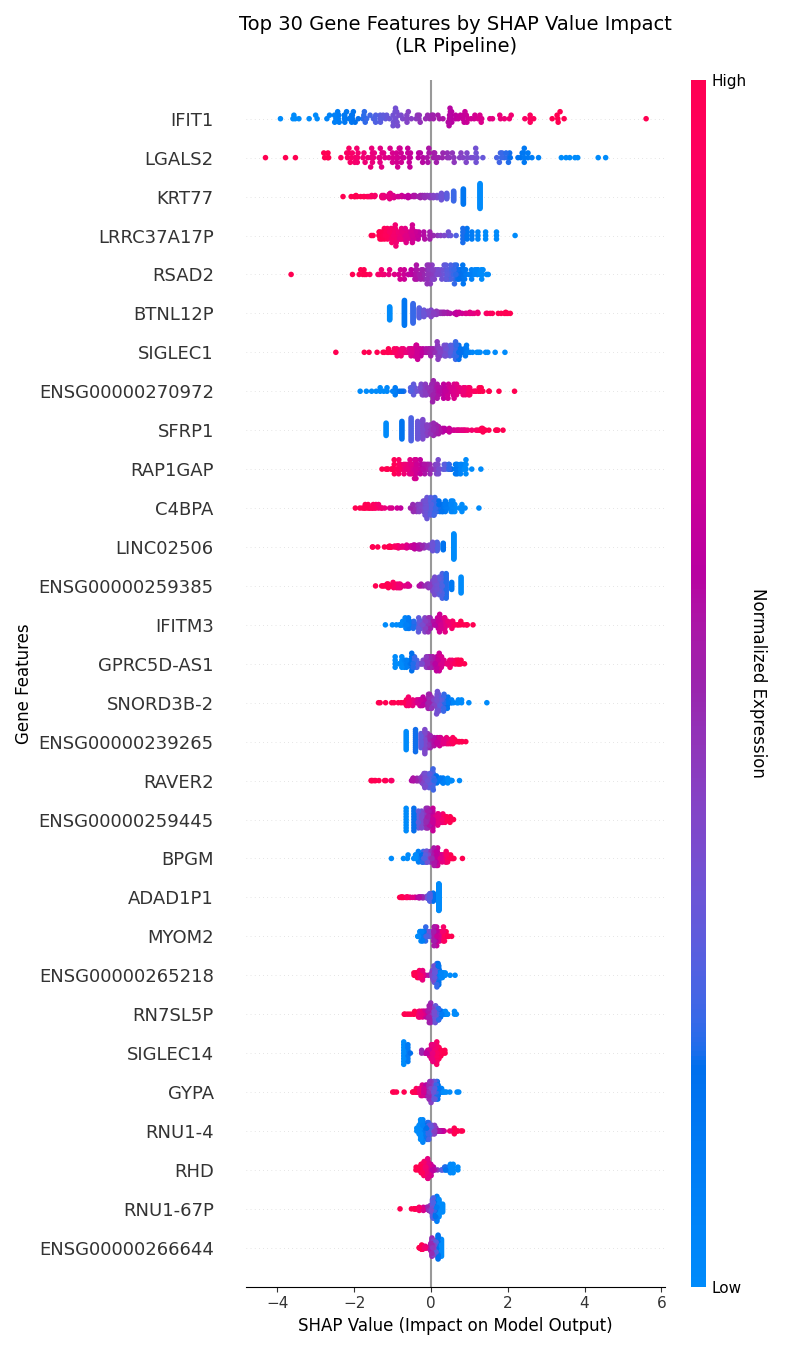
\includegraphics[height=11cm,width=\textwidth,keepaspectratio]{ML/Predict/DEG/SHAP/LR/shap_beeswarm_plot_Female_50-70_useSMOTE_False.png}
                    \caption{Γυναίκες 50-70 ετών}
                    \label{fig:shap_beeswarm_LR_plot_Female_50-70_useSMOTE_False}
                \end{subfigure}
                \hfill
                \begin{subfigure}[b]{0.45\textwidth}
                    \centering
                    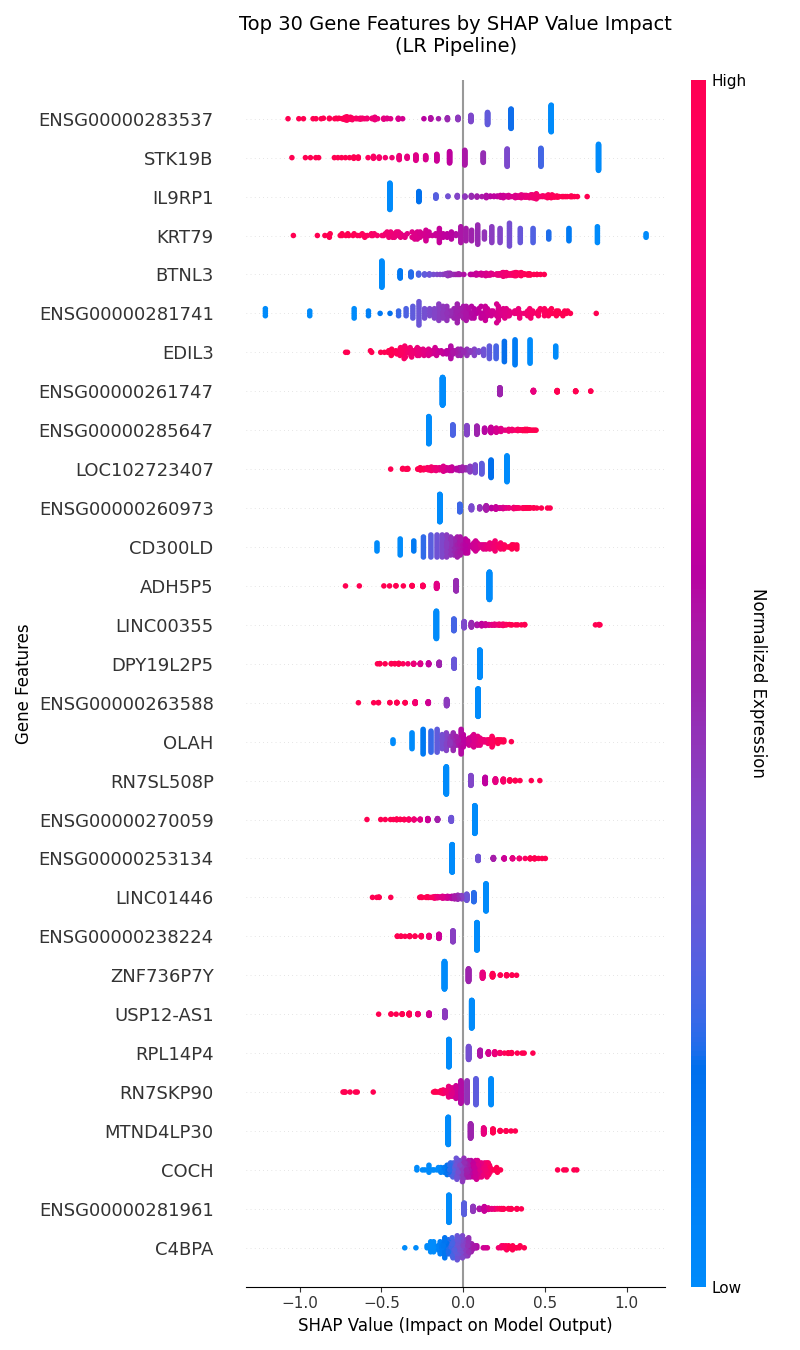
\includegraphics[height=11cm,width=\textwidth,keepaspectratio]{ML/Predict/DEG/SHAP/LR/shap_beeswarm_plot_Male_50-70_useSMOTE_False.png}
                    \caption{Άνδρες 50-70 ετών}
                    \label{fig:shap_beeswarm_LR_plot_Male_50-70_useSMOTE_False}
                \end{subfigure}
                \caption{Ανάλυση SHAP για μοντέλο Λογιστικής Παλινδρόμησης}
                \label{fig:beeswarm-shap-50-70-lr-classifier}
            \end{figure}
        \par
            Συγκρίνοντας τις γραφικές αναπαραστάσεις των εικόνων \ref{fig:shap_beeswarm_LR_plot_Female_50-70_useSMOTE_False} και \ref{fig:shap_beeswarm_LR_plot_Male_50-70_useSMOTE_False}, ιδιαίτερα στις πρώτες εγγραφές από την κορυφή, καθώς εκεί βρίσκονται και τα χαρακτηριστικά που είχαν το μεγαλύτερο αντίκτυπο στην ταξινόμηση, διακρίνονται περισσότερα διαφορετικά γονίδια μεταξύ ανδρών και γυναικών παρά κοινά. Αυτό το φαινόμενο επιτρέπει στο συμπέρασμα, πως η νόσος του Πάρκινσον οδηγείται ενδεχομένως από εκφράσεις διαφορετικών γονιδίων μεταξύ ανδρών και γυναικών.
            
            \begin{figure}[H]
                \centering
                \begin{subfigure}[b]{0.45\textwidth}
                    \centering
                    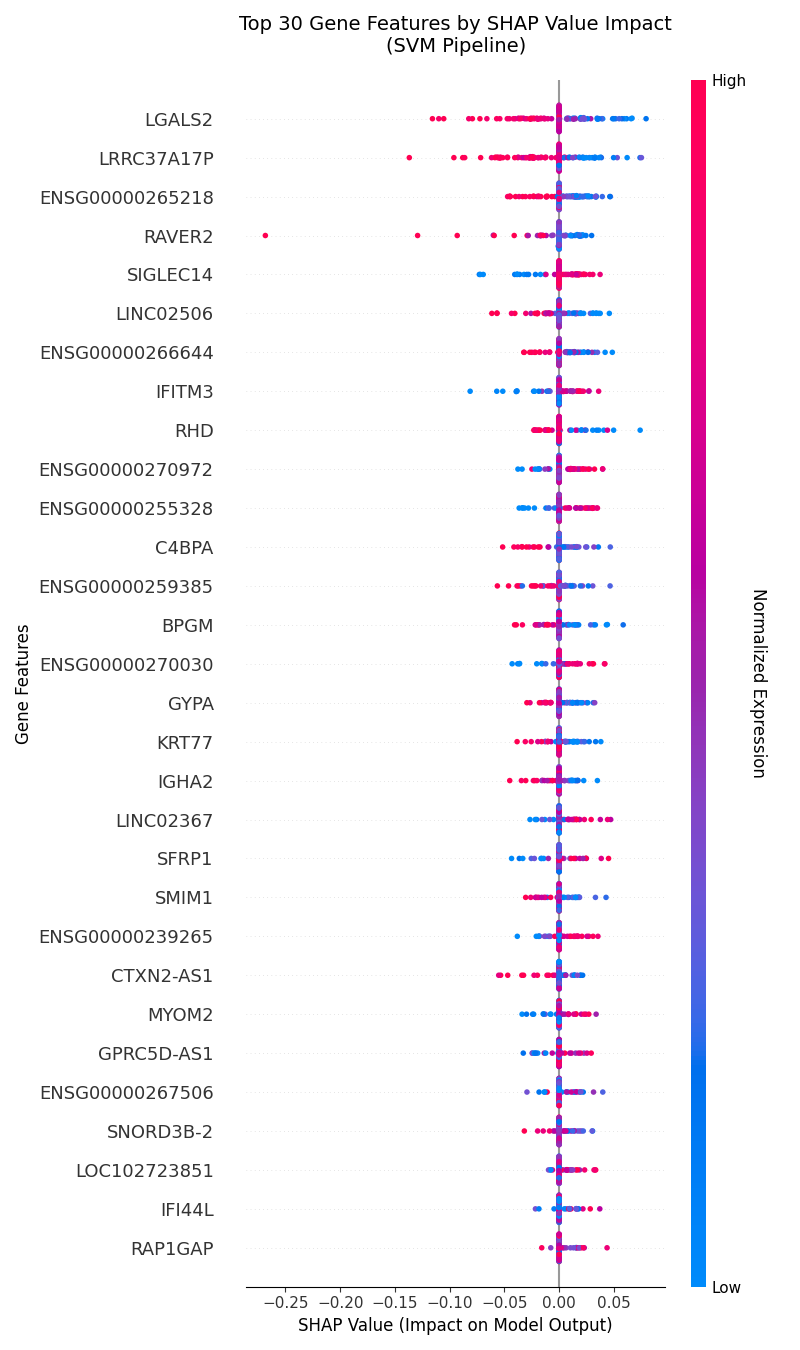
\includegraphics[height=11cm,width=\textwidth,keepaspectratio]{ML/Predict/DEG/SHAP/SVM/shap_beeswarm_plot_Female_50-70_useSMOTE_False.png}
                    \caption{Γυναίκες 50-70 ετών}
                    \label{fig:shap_beeswarm_SVM_plot_Female_50-70_useSMOTE_False}
                \end{subfigure}
                \hfill
                \begin{subfigure}[b]{0.45\textwidth}
                    \centering
                    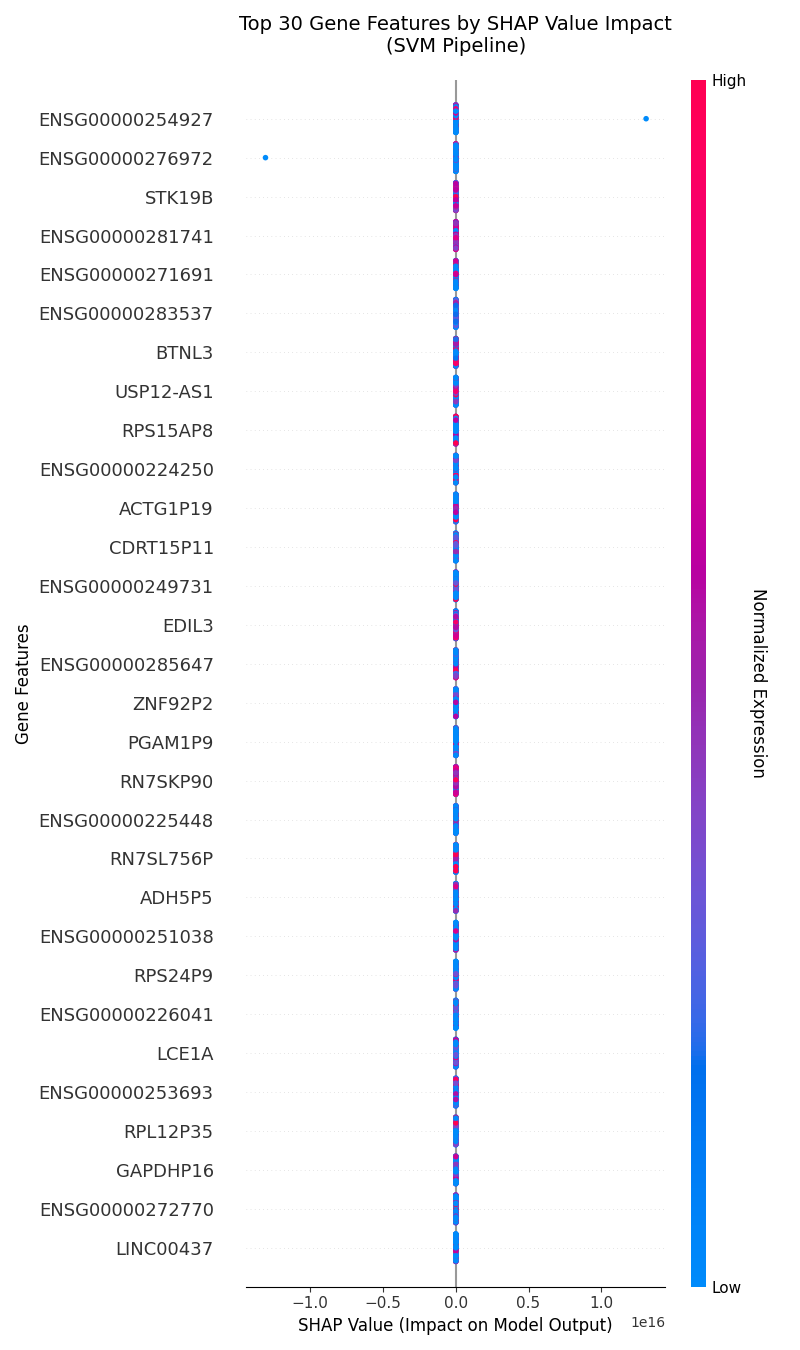
\includegraphics[height=11cm,width=\textwidth,keepaspectratio]{ML/Predict/DEG/SHAP/SVM/shap_beeswarm_plot_Male_50-70_useSMOTE_False.png}
                    \caption{Άνδρες 50-70 ετών}
                    \label{fig:shap_beeswarm_SVM_plot_Male_50-70_useSMOTE_False}
                \end{subfigure}
                \caption{Ανάλυση SHAP για μοντέλο SVM}
                \label{fig:beeswarm-shap-50-70-svm-classifier}
            \end{figure}
        \par
            Το συμπέρασμα από την εφαρμογή της μεθόδου SHAP στα αποτελέσματα της ταξινόμησης μέσω της λογιστικής παλινδρόμησης υποστηρίζεται από τα σημαντικά χαρακτηριστικά που εξάγονται από το μοντέλο SVM. Για τις γυναίκες παρουσιάζονται τα γονίδια LGALS2 και LRRC37A17P ως τα σημαντικότερα. Επίσης, τα αποτελέσματα δείχνουν και συνοχή ως προς το μοτίβο έκφρασης, δηλαδή και τα δύο αυτά γονίδια βοήθησαν να διακριθούν οι νοσούντες από τους υγιείς μέσω χαμηλών επιπέδων έκφρασης και ταυτόχρονα οι υγιείς από τους νοσούντες μέσω υψηλών επιπέδων έκφρασης (\emph{\ref{fig:shap_beeswarm_SVM_plot_Female_50-70_useSMOTE_False}}).
        \par
            Το ίδιο μοτίβο επαναλαμβάνεται και στην περίπτωση του μοντέλου Random Forest, όπου παρουσιάζονται και πάλι τα γονίδια LGALS2 και LRRC37A17P στις ανώτερες θέσεις με τα ίδια μοτίβα έκφρασης τα οποία οδήγησαν και στους προηγούμενους κατηγοριοποιητές την ταξινόμηση (\emph{\ref{fig:shap_beeswarm_RF_plot_Female_50-70_useSMOTE_False}}). Στους άνδρες δείχνουν τα γονίδια ENSG00000283537, STK19B, KRT79 σημαντικότητα σε μοτίβο υπο-έκφρασης για την ομάδα νοσούντων. Αντίθετα, τα γονίδια IL9RP1, ENSG00000281741 και BTNL3 παρουσιάζονται ως οδηγοί διάκρισης της ομάδας νοσούντων σε μοτίβο υπέρ-έκφρασης.
            \begin{figure}[H]
                \centering
                \begin{subfigure}[b]{0.45\textwidth}
                    \centering
                    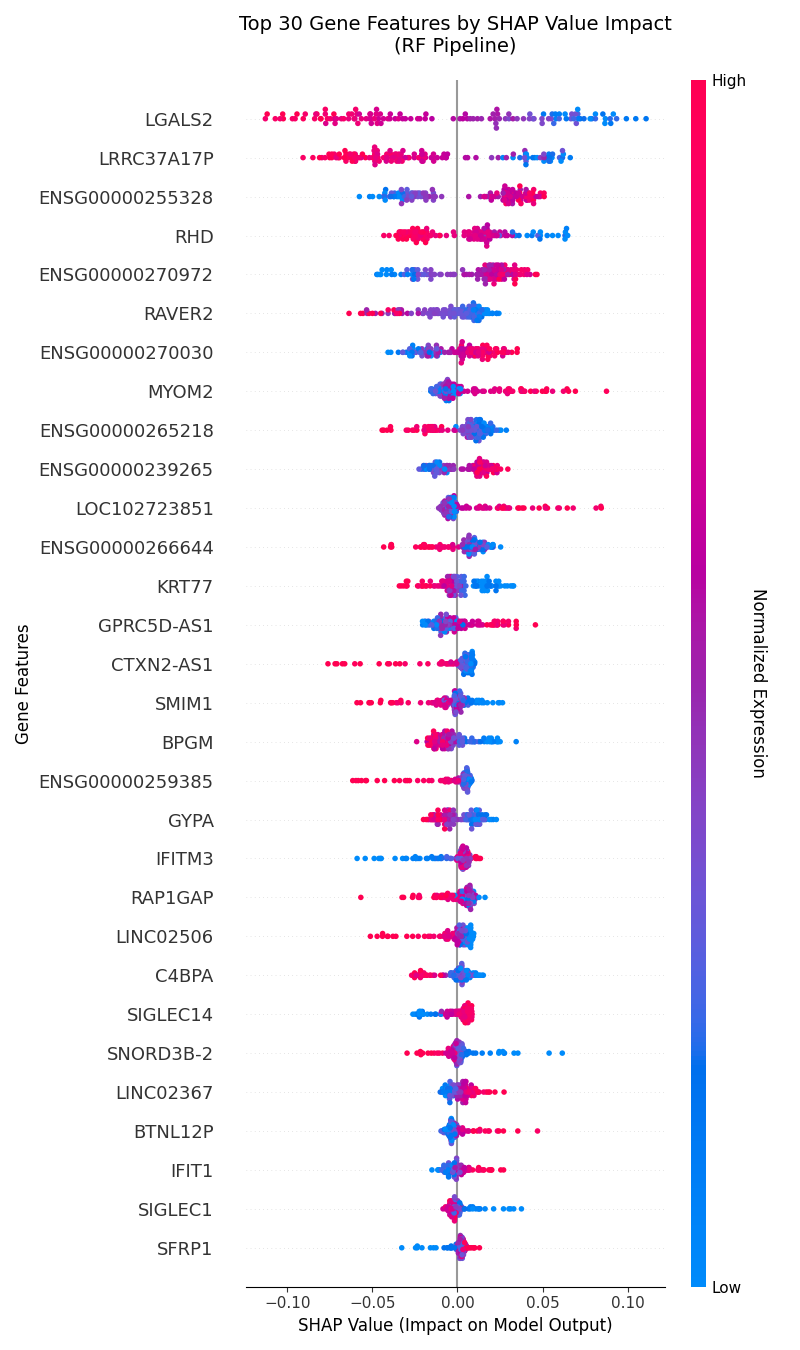
\includegraphics[height=11cm,width=\textwidth,keepaspectratio]{ML/Predict/DEG/SHAP/RF/shap_beeswarm_plot_Female_50-70_useSMOTE_False.png}
                    \caption{Γυναίκες 50-70 ετών}
                    \label{fig:shap_beeswarm_RF_plot_Female_50-70_useSMOTE_False}
                \end{subfigure}
                \hfill
                \begin{subfigure}[b]{0.45\textwidth}
                    \centering
                    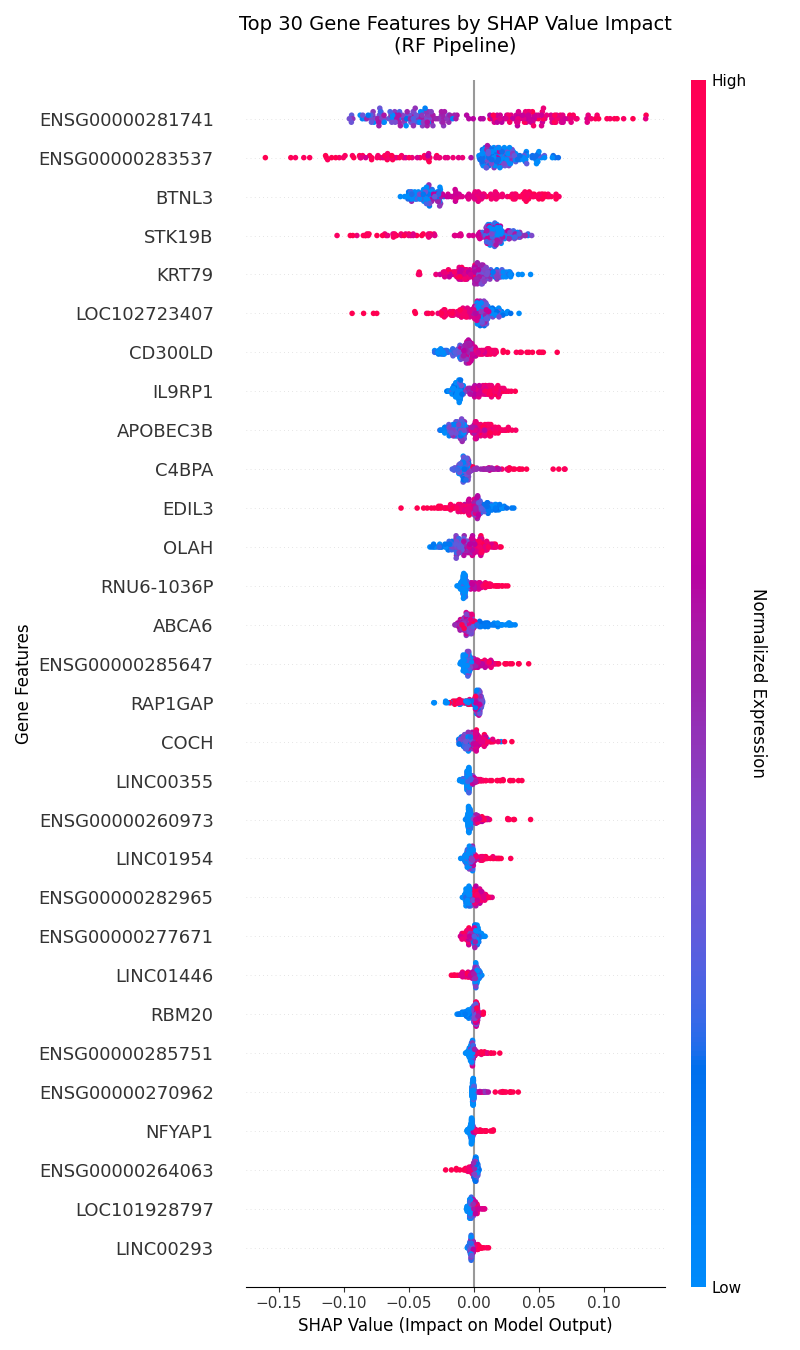
\includegraphics[height=11cm,width=\textwidth,keepaspectratio]{ML/Predict/DEG/SHAP/RF/shap_beeswarm_plot_Male_50-70_useSMOTE_False.png}
                    \caption{Άνδρες 50-70 ετών}
                    \label{fig:shap_beeswarm_RF_plot_Male_50-70_useSMOTE_False}
                \end{subfigure}
                \caption{Ανάλυση SHAP για μοντέλο Random Forest}
                \label{fig:beeswarm-shap-50-70-rf-classifier}
            \end{figure}             
        \par
            Για τον κατηγοριοποιητή XGBoost σημαντικό ρόλο διαδραμάτισε η έκφραση του γονιδίου LGAL2 ενώ το κοινό στους κατηγοριοποιητές της λογιστικής παλινδρόμησης, SVM και Random Forest γονίδιο LRRC37A17P δεν βρίσκεται εντός των πρώτων τριών θέσεων. Αντί αυτού, παρουσιάζονται τα γονίδια ENSG00000239265, C4BPA, GPRC5D-AS1 ως σημαντικότερα, τα οποία στους άλλους κατηγοριοποιητές αποδόθηκε χαμηλότερη σημασία. Τα σημαντικά γονίδια στην ομάδα των ανδρών παρουσιάζουν ομοιότητα στον κατηγοριοποιητή XGBoost (\emph{\ref{fig:shap_beeswarm_XGB_plot_Male_50-70_useSMOTE_False}}) για την αντίστοιχη ομάδα του κατηγοριοποιητή Random Forest (\emph{\ref{fig:shap_beeswarm_RF_plot_Male_50-70_useSMOTE_False}}). Συγκεκριμένα, στις ανώτερες θέσεις βρίσκονται και στους δύο κατηγοριοποιητές τα γονίδια ENSG00000281741, BTNL3 και STK19B.
            \begin{figure}[ht]
                \centering
                \begin{subfigure}[b]{0.45\textwidth}
                    \centering
                    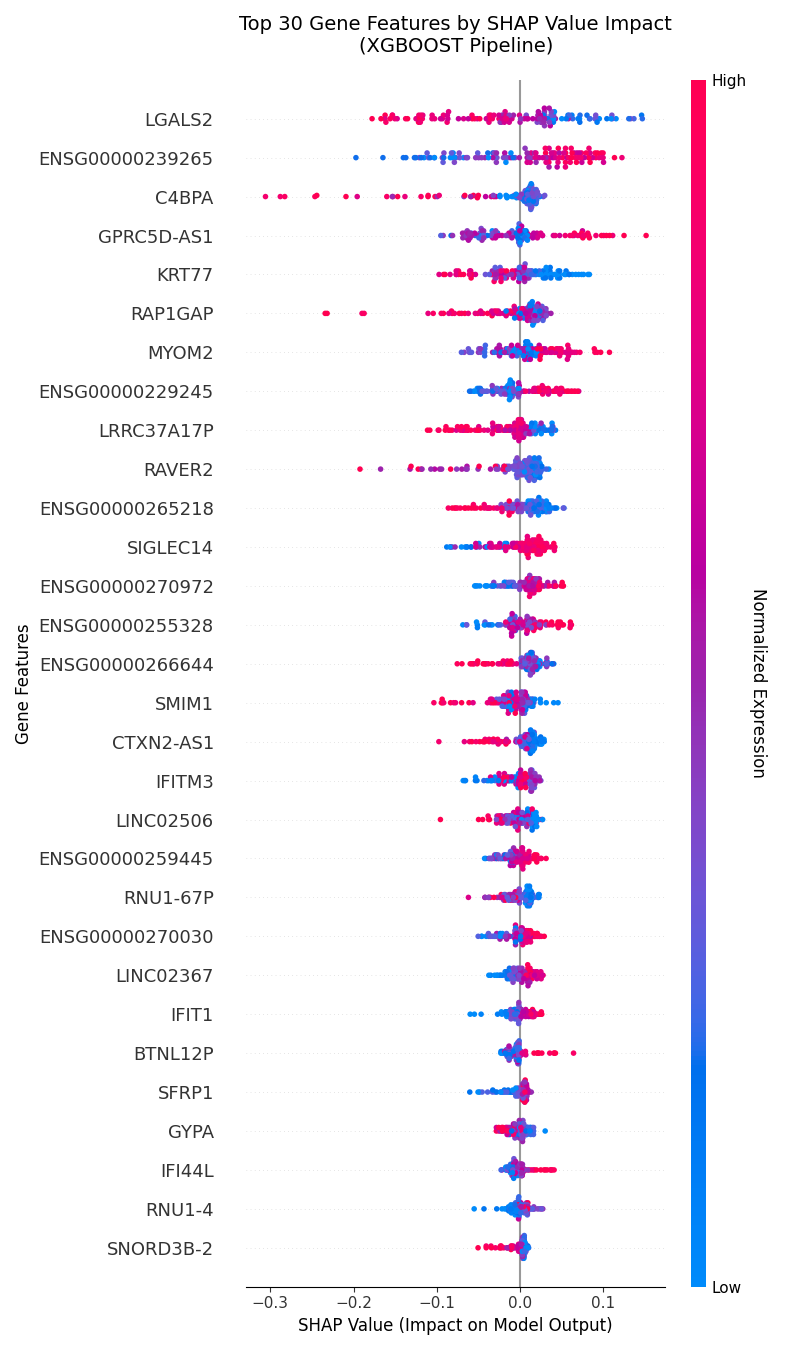
\includegraphics[height=11cm,width=\textwidth,keepaspectratio]{ML/Predict/DEG/SHAP/XGBoost/shap_beeswarm_plot_Female_50-70_useSMOTE_False.png}
                    \caption{Γυναίκες 50-70 ετών}
                    \label{fig:shap_beeswarm_XGB_plot_Female_50-70_useSMOTE_False}
                \end{subfigure}
                \hfill
                \begin{subfigure}[b]{0.45\textwidth}
                    \centering
                    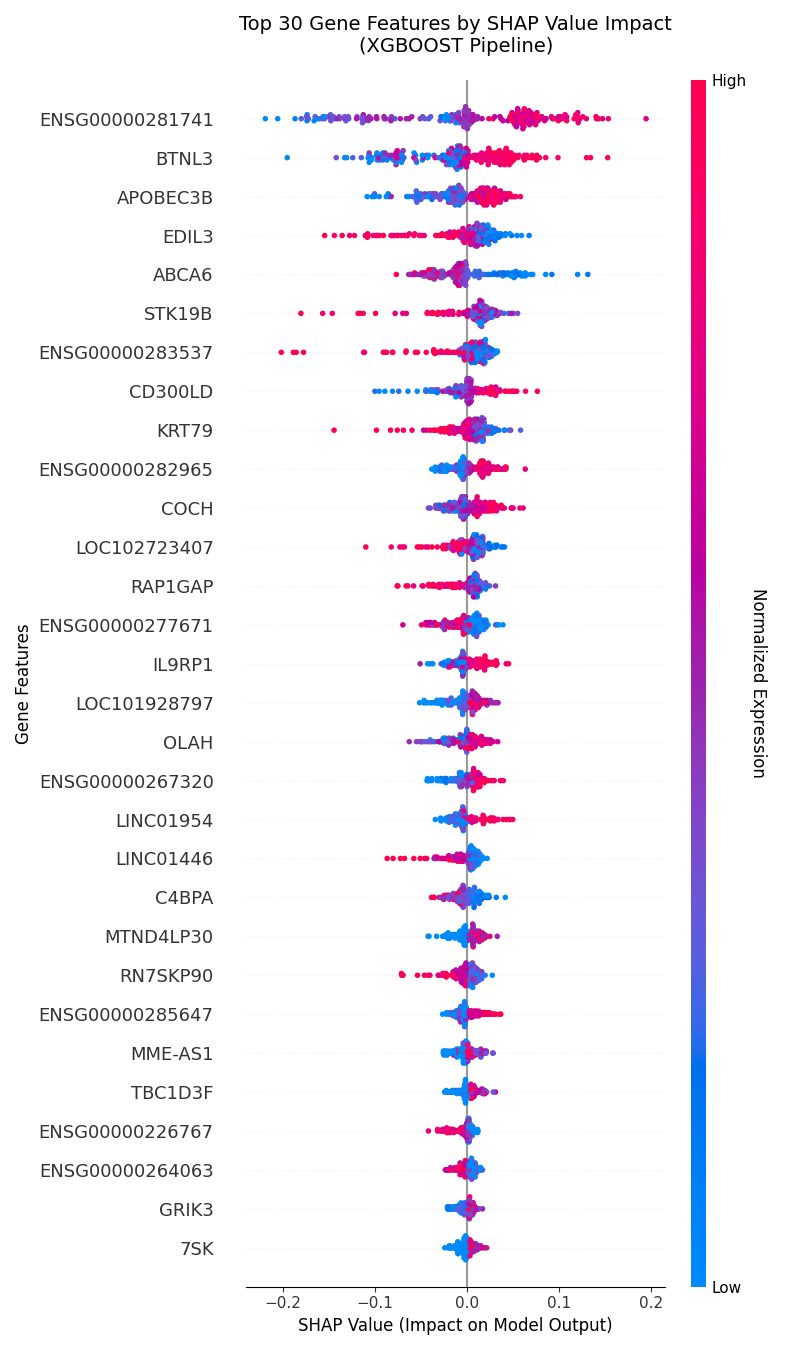
\includegraphics[height=11cm,width=\textwidth,keepaspectratio]{ML/Predict/DEG/SHAP/XGBoost/shap_beeswarm_plot_Male_50-70_useSMOTE_False.png}
                    \caption{Άνδρες 50-70 ετών}
                    \label{fig:shap_beeswarm_XGB_plot_Male_50-70_useSMOTE_False}
                \end{subfigure}
                \caption{Ανάλυση SHAP για μοντέλο Random Forest}
                \label{fig:beeswarm-shap-50-70-xgb-classifier}
            \end{figure}
        \par
            Η εφαρμογή της μεθόδου SHAP στα μοντέλα κατηγοριοποίησης ανά φύλο της ηλικιακής ομάδας 50-70 ετών έδειξε συνοχή ως προς τα γονίδια που συντέλεσαν στην ταξινόμηση και διάκριση μεταξύ δειγμάτων των ομάδων ελέγχου και νοσούντων. Εκτός από την απόδοση παρόμοιων σκορ, διακρίθηκε και η συνοχή στα αντίστοιχα μοτίβα έκφρασης.

    \section{Χαρτογράφηση λειτουργικών δικτύων και ανάλυση εμπλουτισμού}
            Στα πλαίσια της εργασίας διενεργήθηκε η χαρτογράφηση λειτουργικών δικτύων με τη χρήση του λογισμικού Cytoscape (\emph{\cite{Shannon2003Cytoscape:Networks}}) καθώς και ο εμπλουτισμός των αλληλεπιδράσεων και βιβλιογραφίας μέσω της βάσης STRING (\emph{\cite{Szklarczyk2023TheInterest}}) \nomenclature{STRING}{Search Tool for the Retrieval of Interacting Genes/Proteins} και η ανάλυση εμπλουτισμού, με τη χρήση του API \nomenclature{API}{Application Programming Interface} της βάσης Enrichr (\emph{\cite{Chen2013Enrichr:Tool}}) μέσω της βιβλιοθήκης Python GSEApy (\emph{\cite{Fang2023GSEApy:Python}}). Επίσης, χρησιμοποιήθηκε η βάση δεδομένων Gene4PD (\emph{\cite{Li2021Gene4PD:Disease}}) όπου υπάρχουν εμπλουτισμένες καταχωρισμένες συσχετίσεις γονιδίων με τη νόσο του Πάρκινσον από διαδεδομένες βάσεις σχολιασμού. Ο στόχος είναι η αποτίμηση του συνόλου των αποτελεσμάτων, από τα επιμέρους αναλυτικά στάδια που πραγματοποιήθηκαν σε αυτήν την εργασία. Η χαρτογράφηση γονιδιακών δικτύων και η ανάλυση εμπλουτισμού έγιναν με βάση τα διαφορικά εκφραζόμενα γονίδια που προέκυψαν ανά φύλο και ηλικιακή ομάδα.

            \begin{figure}[H]
                \centering
                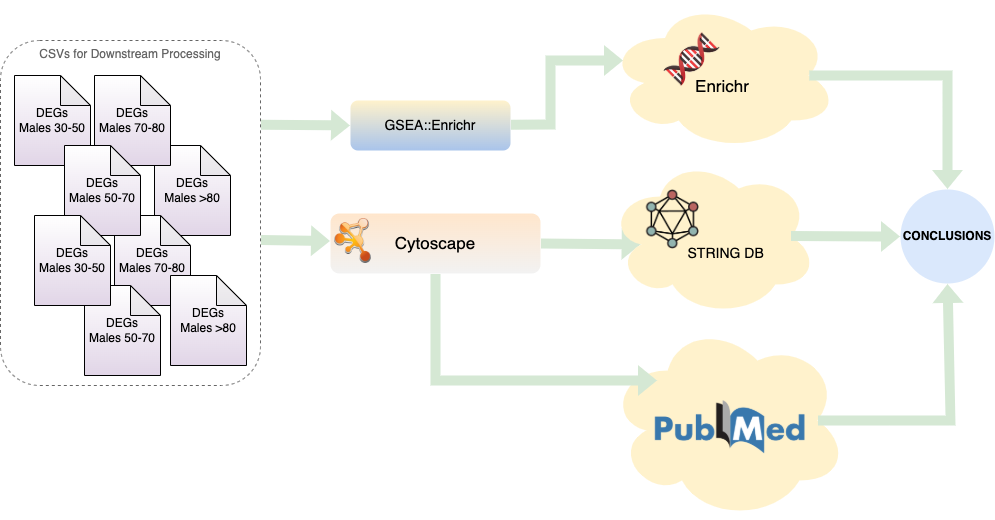
\includegraphics[width=0.7\textwidth]{GSEA/msci-big-pic-GSEA-blocks.png}
                \caption{Pipeline για την χαρτογράφηση λειτουργικών δικτύων και ανάλυση εμπλουτισμού}
                \label{fig:msci-big-pic-GSEA-blocks}
            \end{figure}
    
        \subsection{Αποτελέσματα γυναικών - Ηλικίες 50-70 έτη}
            Στον πίνακα~\ref{tab:cyto-enrichment-females-50-70} παρατίθενται τα αποτελέσματα εμπλουτισμού μετά από κατασκευή δικτύου με βάση διαφορικά εκφραζόμενα γονίδια γυναικών, της ηλικιακής ομάδας 50-70 ετών. Έντονη είναι η παρουσία των γονιδίων IFITM3, SIGLEC1, MYOM2 τα οποία απαντώνται και στα αποτελέσματα της εφαρμογής της μεθόδου SHAP (\emph{εικόνες \ref{fig:shap_beeswarm_LR_plot_Female_50-70_useSMOTE_False}, \ref{fig:shap_beeswarm_SVM_plot_Female_50-70_useSMOTE_False}, \ref{fig:shap_beeswarm_RF_plot_Female_50-70_useSMOTE_False}, \ref{fig:shap_beeswarm_XGB_plot_Female_50-70_useSMOTE_False}}).
        \begin{table}[H]
            \centering
            \scriptsize % Small font size (8pt)
            \setlength{\tabcolsep}{4pt} % Tight column spacing
            \renewcommand{\arraystretch}{1.1} % Slightly increased row spacing
            \begin{tabular}{@{}>{\raggedright}p{3cm}>{\raggedright}p{6cm}cS[table-format=1.2E-2]@{}}
                \toprule
                \textbf{Source} & \textbf{Term Name} & \textbf{Intersecting Genes} & \textbf{P-value} \\
                \midrule
                WikiPathways & Network map of SARS CoV 2 signaling & IFITM3, SIGLEC1, MYOM2 & 1.6E-3 \\
                Gene Ontology (BP) & biological process involved in interaction with host & IFITM3, 9606, ENSP00000371471, SIGLEC1 & 6.6E-3 \\
                Transfac predictions & Factor: IRF-1; motif: INRAAANNGAAASN; match class: 1 & SIGLEC1, MYOM2 & 8.2E-3 \\
                mirTarBase & hsa-miR-146a-5p & IFITM3, SIGLEC1, MYOM2 & 1.06E-2 \\
                Gene Ontology (BP) & biological process involved in symbiotic interaction & IFITM3, l9606.ENSP00000371471, SIGLEC1 & 2.41E-2 \\
                Gene Ontology (BP) & defense response to virus & IFITM3, SIGLEC1, MYOM2 & 2.41E-2 \\
                Reactome & Interferon alpha/beta signaling & IFITM3, SIGLEC1 & 2.60E-2 \\
                Gene Ontology (BP) & viral life cycle & IFITM3, 9606.ENSP00000371471, SIGLEC1 & 2.61E-2 \\
                Transfac predictions & Factor: IRF-4; motif: KRAAANGAAAANYN; match class: 1 & SIGLEC1, MYOM2 & 3.91E-2 \\
                \bottomrule
            \end{tabular}
            \caption{Αποτελέσματα εμπλουτισμού κατά τη χαρτογράφηση γονιδιακών δικτύων γυναικών 50-70 ετών}
            \label{tab:cyto-enrichment-females-50-70}
        \end{table}
            Η εικόνα~\ref{fig:cyto_females_50_70} παρουσιάζει το γονιδιακό δίκτυο, όπως αυτό προέκυψε μετά την ανάλυση μέσω Cytoscape, όπου ο σκούρος χρωματισμός των κόμβων αντιπροσωπεύει υψηλές απόλυτες τιμές έκφρασης και ο ανοιχτός αντίστοιχα χαμηλές τιμές. Χαρακτηριστική στο δίκτυο είναι η παρουσία ιντερφερόνων, η έκφραση των οποίων συμβαδίζει με μια απόκριση του ανοσοποιητικού συστήματος σε φλεγμονή ή και σε κυτταρική βλάβη (\emph{\cite{Kopitar-Jerala2017TheActivation}}). Στα αποτελέσματα βιβλιογραφικού εμπλουτισμού μέσω STRING διακρίθηκαν αποτελέσματα για το υποδίκτυο των γονιδίων RSAD2, IFIT1, SIGLEC1, IFI44L, σχετικά με την κινάση Janus (\emph{\cite{Yamaoka2004TheJaks}}), η οποία συμμετέχει στο μονοπάτι Jak/Stat, με το οποίο βρέθηκε συσχετισμός με έκφραση γονιδίου ιντερφερόνης IF27, που αναφέρθηκε στον πίνακα~\ref{tab:gene4pd-known-genes}. Ο συσχετισμός του μονοπατιού Jak/Stat με τη νόσο του Πάρκινσον περιγράφεται από τους \cite{Lashgari2021TheDisease} ως πιθανός θεραπευτικός στόχος. Ταυτόχρονα το ίδιο υποδίκτυο σχετίζεται με αναφορά σε νευροεκφυλισμό, σύμφωνα με δημοσίευση των \cite{Cooray2023NeuroinflammationIRAK4}.
            \begin{figure}[h]
                \centering
                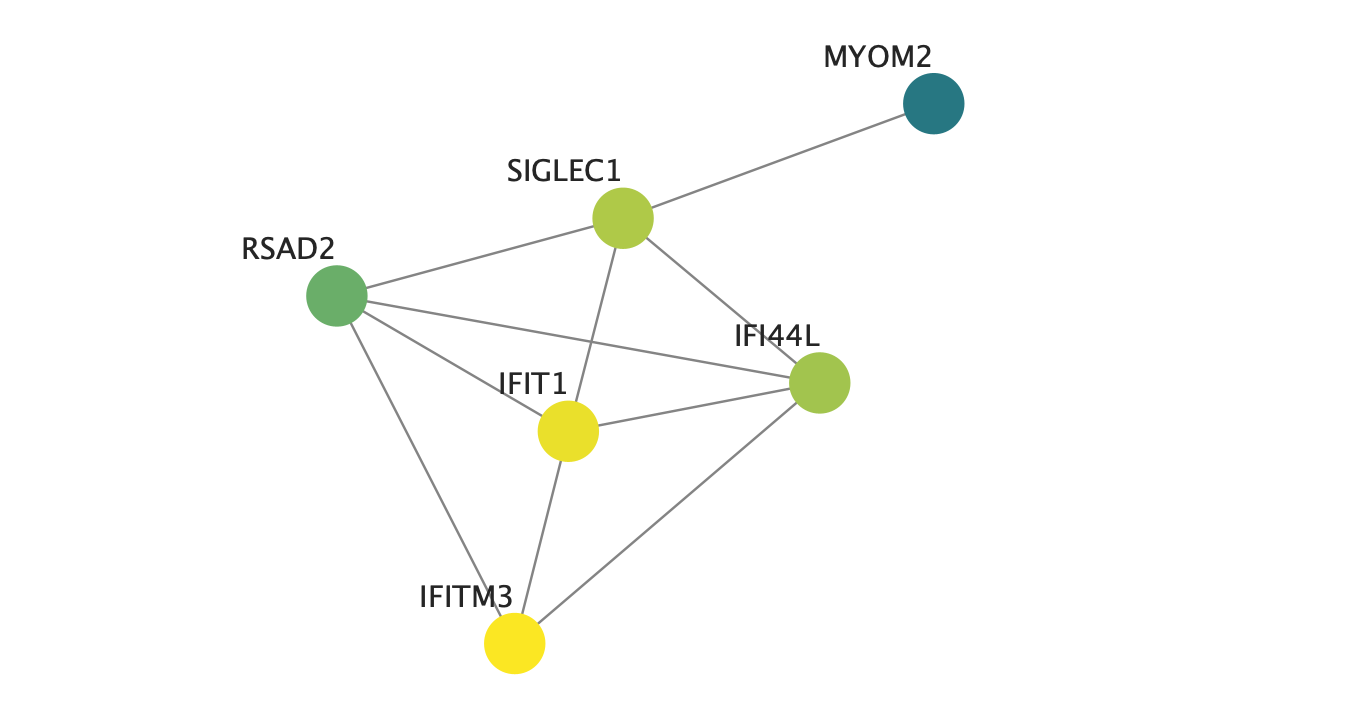
\includegraphics[width=0.65\textwidth]{Cytoscape/cyto_females_50_70.png}
                \caption{Λειτουργικό δίκτυο διαφορικά εκφραζόμενων γονιδίων σε γυναίκες 50-70 ετών}
                \label{fig:cyto_females_50_70}
            \end{figure}
            \begin{table}[H]
                \centering
                \scriptsize
                \setlength{\tabcolsep}{4pt}
                \renewcommand{\arraystretch}{1.1}
                \begin{tabular}{@{}>{\raggedright}p{10cm}S[table-format=1.2E-2]c@{}}
                    \toprule
                    \textbf{Description} & \textbf{FDR} & \textbf{PMID} \\
                    \midrule
                     Janus Kinase Inhibitors in the Treatment of Type I Interferonopathies: A Case Series From a Single Center in China. & 1.75E-5 & PMID:35418997 \\
                      JAK inhibitors: a potential treatment for JDM in the context of the role of interferon-driven pathology. & 7.98E-5 & PMID:34563217 \\
                      Neuroinflammation, autoinflammation, splenomegaly and anemia caused by bi-allelic mutations in IRAK4. & 1.2E-4 & PMID:37744344 \\
                    \bottomrule
                \end{tabular}
                \caption{Επιλογή βιβλιογραφικών αναφορών κατά τη χαρτογράφηση γονιδιακών δικτύων γυναικών 50-70 ετών}
                \label{tab:cyto-pub-enrichment-females-50-70}
            \end{table}
            \newpage
                Τα αποτελέσματα εμπλουτισμού μέσω Enrichr δεν αποκλίνουν από τα παραπάνω, καθώς και σε αυτή την περίπτωση οι σχολιασμοί με υψηλό σκορ στατιστικής σημαντικότητας συγκεντρώνονται γύρω από τη μεταγραφή ιντερφερονών και γενικότερα αφορούν σε λειτουργίες του ανοσοποιητικού. Επιπλέον των βάσεων σχολιασμού οντολογιών και μονοπατιών, συμπεριλήφθηκαν και πηγές δεδομένων από μεταγραφικούς παράγοντες, όπου και πάλι τα αποτελέσματα σχετίζονται ή παραπέμπουν σε αποκρίσεις φλεγμονής (\emph{Πίνακας~\ref{tab:gseapy-enrichment-females-50-70}}). 
            \par
                Χαρακτηριστικό είναι το αποτέλεσμα του μεταγραφικού παράγοντα HESX1\footnote{http://genemed.tech/gene4pd/geneDetail/main?gene\_symbol=HESX1}, για το οποίο βρέθηκαν αντιστοιχήσεις στην βάση Gene4PD με φαινότυπους από την οντολογία HPO \nomenclature{HPO}{Human Phenotype Ontology}(\emph{\cite{Gargano2024TheWorld}}) που αφορούν σε κινητικά προβλήματα, τρόμους, υποσμία και ανοσμία (\emph{\cite{Mitchell2025HyposmiaLoss.}, \cite{Tarakad2017AnosmiaDisease}}), παθολογικά επίπεδα προλακτίνης (που σύμφωνα με \emph{\cite{Al-kuraishy2023TheWays} δεν υφίσταται ακριβή και εξακριβωμένη συσχέτιση}) και κατ' επέκταση σχετικούς με τη νόσο του Πάρκινσον (\emph{Πίνακας~\ref{tab:hpo-terms-females-50-70}}).
            \begin{table}[H]
                \centering
                \scriptsize
                \setlength{\tabcolsep}{4pt}
                \renewcommand{\arraystretch}{1.1}
                \begin{tabular}{@{}
                    >{\raggedright}p{4.5cm}
                    >{\raggedright}p{3cm}S[table-format=1.2E-2]
                    >{\raggedright\arraybackslash}p{2.5cm}
                    @{}
                }
                    \toprule
                    \textbf{Gene set} & \textbf{Term} & \textbf{Adjusted P-value} & \textbf{Genes} \\
                    \midrule
                    MSigDB\_Hallmark\_2020 & Interferon Gamma Response & 7.0E-4 & IFITM3, RSAD2, BPGM, IFIT1, IFI44L \\
                    MSigDB\_Hallmark\_2020 & Interferon Alpha Response & 4.3E-3 & IFITM3, RSAD2, IFI44L \\
                    Enrichr\_Submissions\_TF-Gene\_Coocurrence & \textbf{HESX1} & 5.19E-2 & IFITM3, RSAD2, SIGLEC1, IFIT1, IFI44L \\
                    \bottomrule
                \end{tabular}
                \caption{Ανάλυση εμπλουτισμού μέσω Enrichr - ενδεικτικά αποτελέσματα γυναικών 50-70 ετών}
                \label{tab:gseapy-enrichment-females-50-70}
            \end{table}

            \begin{table}[H]
                \centering
                \scriptsize
                \setlength{\tabcolsep}{4pt}
                \renewcommand{\arraystretch}{1.1}
                \begin{tabular}{@{}>{\raggedright}p{5cm}c@{}}
                    \toprule
                    \textbf{HP ID} & \textbf{Phenotype} \\
                    \midrule
                    HP:0001337 & Tremor \\
                    HP:0001288 & Gait disturbance \\
                    HP:0004409 & Hyposmia \\
                    HP:0000458 & Anosmia \\
                    HP:0040086 & Abnormal prolactin level \\
                    HP:0008202 & Reduced circulating prolactin concentration \\
                    \bottomrule
                \end{tabular}
                \caption{Σχετικοί με τη νόσο του Πάρκινσον Φαινότυποι σε έδαφος του μεταγραφικού παράγοντα HSX1}
                \label{tab:hpo-terms-females-50-70}
            \end{table}
        \subsection{Αποτελέσματα ανδρών - Ηλικίες 50-70 έτη}
            Τα αποτελέσματα της ανάλυσης λειτουργικών δικτύων μέσω Cytoscape για τα διαφορικά εκφραζόμενα γονίδια ανδρών της ηλικιακής ομάδας 50-70 ετών χαρακτηρίζονται από την έντονη παρουσία πρωτεϊνών κερατίνης (\emph{Εικόνα~\ref{fig:cyto_males_keratin_50_70}}). Σύμφωνα με τα ευρήματα της διαφορικής ανάλυσης, το γονίδιο KRT77 βρέθηκε να υπό-εκφράζεται και επίσης συνέβαλε στη διαφοροποίηση μεταξύ παθολογικών και υγιών δειγμάτων στην εφαρμογή ταξινόμησης μηχανικής μάθησης. Παραδόξως, τα παρακάτω απεικονιζόμενα γονίδια παρουσιάζουν υπέρ-έκφραση (\emph{σκούρος χρωματισμός των κόμβων}).  Έρευνες που έχουν αποτυπωθεί σε δημοσιεύσεις όπως των \cite{Liu2025ImpairedKeratinocytes} και \cite{Wang2022BioinformaticsDisease} αναφέρουν μεταξύ άλλων και το αντίκτυπο σε επίπεδα κερατίνης στη νόσο του Πάρκινσον. Χαρακτηριστική είναι η απουσία οποιουδήποτε στοιχείου απόκρισης ανοσοποιητικού συστήματος ή κάποιου σχολιασμού σχετικά με φλεγμονή, σε αντίθεση με τους όρους εμπλουτισμού που σχημάτιζαν την πλειοψηφία του συνόλου του εμπλουτισμού στις γυναίκες. Από τον εμπλουτισμό βιβλιογραφίας μέσω της βάσης STRING δεν προέκυψαν αποτελέσματα, παρά μόνο για τη λειτουργική ανάλυση εμπλουτισμού.         Στον πίνακα~\ref{tab:cyto-enrichment-males-50-70} παρατίθενται τα αποτελέσματα της λειτουργικής ανάλυσης εμπλουτισμού μέσω STRING. Όλα τα αποτελέσματα αφορούν βιολογικές διεργασίες σχετικές με την κερατίνη. Στις σχετικές διεργασίες συμβάλλουν κατ' επανάληψη γονίδια όπως LCE1A, LC5AA (\emph{οικογένεια πρωτεϊνών Late Cornified Envelope}) και οι σχετικές με την πρωτεΐνη της κερατίνης KRTAP45, KRTAP21, κοκ. 
            \begin{figure}[H]
                \centering
                \includegraphics[width=0.5\textwidth]{Cytoscape/Males/cyto_males_50_70_keratine.png}
                \caption{Λειτουργικό δίκτυο διαφορικά εκφραζόμενων γονιδίων σε άνδρες 50-70 ετών}
                \label{fig:cyto_males_keratin_50_70}
            \end{figure}
    \begingroup
    \scriptsize
    \setlength{\tabcolsep}{6pt} % Increased from 4pt
    \renewcommand{\arraystretch}{1.1}
    \begin{longtable}{
        @{}
        >{\raggedright}p{3.2cm} % Wider first column
        >{\raggedright}p{3cm}   % Wider second column
        S[table-format=1.2E-2]
        >{\raggedright\arraybackslash}p{6cm} % Widest column
        @{}
    }
        \caption{Αποτελέσματα λειτουργικού εμπλουτισμού - Άνδρες 50-70 ετών}\label{tab:cyto-enrichment-males-50-70}\\
        \toprule
        \textbf{Category} & \textbf{Description} & \textbf{FDR value} & \textbf{Genes} \\
        \midrule
        \endfirsthead

        \toprule
        \textbf{Category} & \textbf{Description} & \textbf{FDR value} & \textbf{Genes} \\
        \midrule
        \endhead

        \midrule
        \multicolumn{4}{r@{}}{\footnotesize\itshape Συνέχεια στην επόμενη σελίδα}\\
        \endfoot

        \bottomrule
        \endlastfoot

        Reactome Pathways & Keratinization & 1.36E-14 & LCE1A, LC5AA, KRTAP4\-5, SPRR2B, IVL, LCECC, KRTAP1\-4, KRTAP13\-3, KRTAP2\-1, KRTAP2\-2, LC5BA \\ 
        Pfam & Keratin, high sulfur B2 protein & 8.27E-11 & KRTAP4\-5, KRTAP1\-4, KRTAP4\-4, KRTAP2\-1, KRTAP9\-9, KRTAP4\-12, KRTAP2\-2 \\ 
        UniProt Keywords & Keratinization & 1.06E-09 & LCE1A, LC5AA, SPRR2B, IVL, LCECC, LC5BA \\ 
        STRING Clusters & Keratin & 2.32E-09 & KRTAP4\-5, KRTAP1\-4, KRTAP4\-4, KRTAP13\-3, KRTAP2\-1, KRTAP9\-9, KRTAP4\-12 \\ 
        GO Cellular Component & Keratin filament & 7.04E-09 & KRTAP4\-5, KRTAP1\-4, KRTAP4\-4, KRTAP2\-1, KRTAP9\-9, KRTAP4\-12, KRTAP2\-2 \\ 
        GO Cellular Component & Intermediate filament & 7.15E-09 & KRTAP4\-5, KRTAP1\-4, KRTAP4\-4, KRTAP13\-3, KRTAP2\-1, KRTAP9\-9, KRTAP4\-12, KRTAP2\-2 \\ 
        STRING Clusters & Keratinization and Cornified envelope & 1.74E-08 & LCE1A, LC5AA, SPRR2B, IVL, LCECC, LC5BA \\ 
        STRING Clusters & Keratin, high sulfur B2 protein & 1.95E-09 & KRTAP4\-5, KRTAP4\-4, KRTAP2\-1, KRTAP9\-9, KRTAP4\-12 \\ 
        STRING Clusters & Keratinization & 3.48E-08 & LCE1A, LC5AA, SPRR2B, LCECC, LC5BA \\ 
        TISSUES & Scalp & 4.42E-08 & KRTAP4\-5, KRTAP4\-4, KRTAP2\-1, KRTAP9\-9, KRTAP4\-12, KRTAP2\-2 \\ 
        STRING Clusters & Late cornified envelope & 7.12E-07 & LCE1A, LC5AA, LCECC, LC5BA \\ 
        STRING Clusters & Keratin, high sulfur B2 protein & 1.01E-08 & KRTAP4\-5, KRTAP4\-4, KRTAP2\-1, KRTAP9\-9 \\ 
        Reactome Pathways & Formation of the cornified envelope & 1.16E-06 & LCE1A, LC5AA, SPRR2B, IVL, LCECC, LC5BA \\ 
        GO Biological Process & Keratinization & 1.99E-06 & LCE1A, LC5AA, SPRR2B, IVL, LCECC, LC5BA \\ 
        STRING Clusters & Late cornified envelope & 9.07E-06 & LCE1A, LCECC, LC5BA \\ 
        TISSUES & Skin & 1.66E-05 & KRTAP4\-5, APOD, SPRR2B, IVL, KRTAP4\-4, KRTAP2\-1, KRTAP9\-9, KRTAP4\-12, KRTAP2\-2, LC5BA \\ 
        UniProt Keywords & Keratin & 6.13E-05 & KRTAP4\-5, KRTAP1\-4, KRTAP13\-3, KRTAP2\-1, KRTAP2\-2 \\ 
        InterPro Domains & Keratin-associated protein & 3.80E-04 & KRTAP4\-5, KRTAP1\-4, KRTAP2\-1, KRTAP2\-2 \\ 
        Pfam & Late cornified envelope & 9.70E-04 & LCE1A, LC5AA, LCECC \\ 
        InterPro Domains & Late cornified envelope protein & 3.00E-03 & LCE1A, LC5AA, LCECC \\ 
        STRING Clusters & Keratin, high sulfur B2 protein & 5.00E-03 & KRTAP4\-5, KRTAP4\-4 \\ 
        STRING Clusters & Mixed, incl. Keratin, high sulfur B2 protein, and Keratin, high-sulphur matrix protein & 5.00E-03 & KRTAP2\-1, KRTAP9\-9 \\ 
        GO Cellular Component & Cytoskeleton & 2.38E-02 & KRTAP4\-5, IVL, KRTAP1\-4, KRTAP4\-4, KRTAP13\-3, KRTAP2\-1, KRTAP9\-9, KRTAP4\-12, KRTAP2\-2 \\ 
        STRING Clusters & Keratin-associated protein, PMG type, and Keratin-associated protein, type6/6/16/19/20/21 & 3.92E-02 & KRTAP1\-4, KRTAP13\-3 \\ 
    \end{longtable}
\endgroup
    Аπό την ανάλυση εμπλουτισμού με τη χρήση Enrichr δεν προέκυψαν στατιστικά σημαντικά αποτελέσματα. Μια επιλογή από τα αποτελέσματα που θα μπορούσαν να θεωρηθούν σχετικά με τη νόσο του Πάρκινσον, λόγω της συνάφειας των εμπλουτισμένων όρων, παρατίθεται στον πίνακα~\ref{tab:enrichr-males-50-70}. 
    \par
        Οι τέσσερις πρώτες εγγραφές αναφέρονται σε κυτταρικές συστάσεις και βιολογικές διεργασίες του νευρικού συστήματος. Η σχέση της εγγραφής IL-2/STAT5 Signaling αφορά σε διεργασία του ανοσοποιητικού συστήματος. Η εγγραφή Xenobiotic Metabolism αναφέρεται σε μεταβολισμό ξενοβιοτικών, δηλαδή εξωσωματικά χημικά τα οποία μπορούν να παρέμβουν στον μεταβολισμό και ως συγκεντροτικός όρος μπορεί να περιλαμβάνει χημικές ουσίες όπως παρασιτοκτόνα αλλά και φάρμακα (\emph{\cite{Croom2012MetabolismEnvironments}}). Η σχέση παρασιτοκτόνων και ανάπτυξης της νόσου έχει αναλυθεί και στο παρελθόν από τους \cite{LeCouteur1999PesticidesDisease}. Η σχέση μεταξύ της νόσου του Πάρκινσον και του μεταβολισμού λιπαρών οξέων αναλύεται από τους \cite{Alecu2019DysregulatedDisease}. Διαταραχές του μεταβολισμού της αίμης και σχέσεις με νευροεκφυλιστικές νόσους, λόγω οξειδωτικού στρές περιγράφεται σε δημοσίευση των \cite{Chiabrando2018UnravelingNeurodegeneration}. Ακολοθούν εγγραφές, κυρίως σχετικές με ανοσολογική απόκριση σε μόλυνση από τον ιό SARS CoV2 καθώς και συγκεκριμένα μετά-COVID προκληθείσα νευροφλεγμονή και χρόνιο οξειδωτικό στρές. Ο εμπλουτισμός για το γονίδιο TUBB8 βρίσκει συσχέτιση με μονοπάτι παρκίνης και ουβικουιτίνης, με ρόλο στην αποδόμηση πρωτεϊνών και διαταραχές της οποίας εικάζεται πως σχετίζεται με τη συσσώρευση  συνουκλεϊνης-α λόγω ελλιπής αποδόμησης και στη συνέχεια την εκδήλωση του νευροεκφυλισμού στη νόσο του Πάρκινσον (\emph{\cite{Zhao2024ExploringDisease}}). Η ομοιόσταση χαλκού, που αναφέρεται ως πρώτη των τεσσάρων τελευταίων εγγραφών του πίνακα, αναφέρεται στη βιβλιογραφία σε δημοσίευση των \cite{Gaggelli2006CopperSclerosis} όπου σχετίζεται με νευροεκφυλιστικές παθήσεις και αναλύει βιοχημικές σχέσεις μεταξύ ιόντων χαλκού και συνουκλεϊνης-α. Στις τρείς τελευταίες εγγραφές αναφέρεται και η νόσος Alzheimer και τέλος ο εμπλουτισμός του γονιδίου TUBB8 με τη νόσο του Πάρκινσον.
    \begin{table}[htbp]
        \centering
        \scriptsize
        \setlength{\tabcolsep}{4pt}
        \renewcommand{\arraystretch}{1.1}
        \begin{tabular}{@{}>{\raggedright}p{3.2cm}>{\raggedright}p{8cm}S[table-format=1.2]>{\raggedright\arraybackslash}p{1.5cm}@{}}
            \toprule
            \textbf{Gene set} & \textbf{Term} & \textbf{Adj. P-value} & \textbf{Genes} \\ \addlinespace
            \midrule
            SynGO\_2024 & Integral Component Of Postsynaptic Density Membrane (GO:0099061) CC & 0.9998 & GRIK3 \\ \addlinespace
            SynGO\_2024 & Voltage-Gated Ca Channel Activity Involved In Regulation Of Presynaptic Cytosolic Ca Levels (GO:0099626) BP & 0.9998 & CACNB2 \\ \addlinespace
            SynGO\_2024 & Ligand-Gated IC Activity Involved In Regulation Of Presynaptic Membrane Potential (GO:0099507) BP & 0.9998 & GRIK3 \\ \addlinespace
            SynGO\_2024 & Integral Component Of Presynaptic Membrane (GO:0099056) CC & 0.9998 & GRIK3 \\ \addlinespace
            MSigDB\_Hallmark\_2020 & IL-2/STAT5 Signaling & 1.0000 & COCH \\ \addlinespace
            MSigDB\_Hallmark\_2020 & Xenobiotic Metabolism & 1.0000 & RAP1GAP \\ \addlinespace
            MSigDB\_Hallmark\_2020 & Fatty Acid Metabolism & 1.0000 & XIST \\ \addlinespace
            MSigDB\_Hallmark\_2020 & Heme Metabolism & 1.0000 & RAP1GAP \\ \addlinespace
            WikiPathways\_2024\_Human & Zinc Homeostasis WP3529 & 1.0000 & MT4 \\ \addlinespace
            WikiPathways\_2024\_Human & Post COVID Neuroinflammation WP5485 & 1.0000 & ACE2 \\ \addlinespace
            WikiPathways\_2024\_Human & SARS CoV 2 Mt Chronic Ox Stress And Endothelial Dysfunction WP5183 & 1.0000 & ACE2 \\ \addlinespace
            WikiPathways\_2024\_Human & COVID 19 Structural Coverage Map WP5145 & 1.0000 & ACE2 \\ \addlinespace
            WikiPathways\_2024\_Human & RAS And Bradykinin Pathways in COVID 19 WP4969 & 1.0000 & ACE2 \\ \addlinespace
            WikiPathways\_2024\_Human & Antiviral And Anti-Inflam Effects Of Nrf2 On SARS CoV 2 Pathway WP5113 & 1.0000 & ACE2 \\ \addlinespace
            WikiPathways\_2024\_Human & Type I Interferon Induction And Signaling SARS CoV 2 Infection WP4868 & 1.0000 & ACE2 \\ \addlinespace
            WikiPathways\_2024\_Human & SARS Coronavirus And Innate Immunity WP4912 & 1.0000 & ACE2 \\ \addlinespace
            WikiPathways\_2024\_Human & Mitochondrial Immune Response To SARS CoV 2 WP5038 & 1.0000 & ACE2 \\ \addlinespace
            WikiPathways\_2024\_Human & lncRNA In Canonical Wnt Signaling And Colorectal Cancer WP4258 & 1.0000 & ROR1;WNT3 \\ \addlinespace
            WikiPathways\_2024\_Human & SARS CoV 2 Innate Immunity Evasion And Cell Immune Response WP5039 & 1.0000 & ACE2 \\ \addlinespace
            WikiPathways\_2024\_Human & Parkin Ubiquitin Proteasomal System Pathway WP2359 & 1.0000 & TUBB8 \\ \addlinespace
            WikiPathways\_2024\_Human & Copper Homeostasis WP3286 & 1.0000 & MT4 \\ \addlinespace
            WikiPathways\_2024\_Human & Alzheimer's Disease WP5124 & 1.0000 & TUBB8;WNT3 \\ \addlinespace
            WikiPathways\_2024\_Human & Alzheimer's Disease And miRNA Effects WP2059 & 1.0000 & TUBB8;WNT3 \\ \addlinespace
            KEGG\_2021\_Human & Parkinson disease & 1.0000 & TUBB8 \\ \addlinespace
            \bottomrule
        \end{tabular}
        \caption{Ανάλυση εμπλουτισμού μέσω Enrichr - ενδεικτικά αποτελέσματα ανδρών 50-70 ετών}
        \label{tab:enrichr-males-50-70}
    \end{table}    
    % \begingroup
    %     \scriptsize
    %     \setlength{\tabcolsep}{4pt}
    %     \renewcommand{\arraystretch}{1.1}
    %     \begin{longtable}{@{}>{\raggedright}p{2.5cm}>{\raggedright}p{4.5cm}S[table-format=1.4]>{\raggedright\arraybackslash}p{2cm}@{}}
    %         \caption{Ανάλυση εμπλουτισμού μέσω Enrichr - ενδεικτικά αποτελέσματα γυναικών 50-70 ετών}\label{tab:enrichr-results-males-50-70}\\
    %         \toprule
    %         \textbf{Gene set} & \textbf{Term} & \textbf{Adj. P-value} & \textbf{Genes} \\
    %         \midrule
    %         \endfirsthead
    
    %         \toprule
    %         \textbf{Gene set} & \textbf{Term} & \textbf{Adj. P-value} & \textbf{Genes} \\
    %         \midrule
    %         \endhead
    
    %         \bottomrule
    %         \multicolumn{4}{r@{}}{\footnotesize\itshape Continued on next page}\\
    %         \endfoot
    
    %         \bottomrule
    %         \endlastfoot
    
    %         \rowcolor{gray!10}
    %         \multirow{4}{*}{SynGO\_2024} & Integral Component Of Postsynaptic Density Membrane (GO:0099061) CC & 0.9998 & GRIK3 \\ 
    %         & Voltage-Gated Ca Channel Activity Involved In Regulation Of Presynaptic Cytosolic Ca Levels (GO:0099626) BP & 0.9998 & CACNB2 \\ 
    %         & Ligand-Gated IC Activity Involved In Regulation Of Presynaptic Membrane Potential (GO:0099507) BP & 0.9998 & GRIK3 \\ 
    %         & Integral Component Of Presynaptic Membrane (GO:0099056) CC & 0.9998 & GRIK3 \\ \cline{2-4}
    
    %         \rowcolor{gray!10}
    %         \multirow{4}{*}{MSigDB\_Hallmark\_2020} & IL-2/STAT5 Signaling & 1.0000 & COCH \\ 
    %         & Xenobiotic Metabolism & 1.0000 & RAP1GAP \\ 
    %         & Fatty Acid Metabolism & 1.0000 & XIST \\ 
    %         & Heme Metabolism & 1.0000 & RAP1GAP \\ \cline{2-4}
    
    %         \rowcolor{gray!10}
    %         \multirow{12}{*}{WikiPathways\_2024\_Human} & Zinc Homeostasis WP3529 & 1.0000 & MT4 \\ 
    %         & Post COVID Neuroinflammation WP5485 & 1.0000 & ACE2 \\ 
    %         & SARS CoV 2 Mt Chronic Ox Stress And Endothelial Dysfunction WP5183 & 1.0000 & ACE2 \\ 
    %         & COVID 19 Structural Coverage Map WP5145 & 1.0000 & ACE2 \\ 
    %         & RAS And Bradykinin Pathways in COVID 19 WP4969 & 1.0000 & ACE2 \\ 
    %         & Antiviral And Anti-Inflam Effects Of Nrf2 On SARS CoV 2 Pathway WP5113 & 1.0000 & ACE2 \\ 
    %         & Type I Interferon Induction And Signaling SARS CoV 2 Infection WP4868 & 1.0000 & ACE2 \\ 
    %         & SARS Coronavirus And Innate Immunity WP4912 & 1.0000 & ACE2 \\ 
    %         & Mitochondrial Immune Response To SARS CoV 2 WP5038 & 1.0000 & ACE2 \\ 
    %         & lncRNA In Canonical Wnt Signaling And Colorectal Cancer WP4258 & 1.0000 & ROR1;WNT3 \\ 
    %         & SARS CoV 2 Innate Immunity Evasion And Cell Immune Response WP5039 & 1.0000 & ACE2 \\ 
    %         & Parkin Ubiquitin Proteasomal System Pathway WP2359 & 1.0000 & TUBB8 \\ \cline{2-4}
    
    %         \rowcolor{gray!10}
    %         WikiPathways\_2024\_Human & Copper Homeostasis WP3286 & 1.0000 & MT4 \\ 
    %         & Alzheimer's Disease WP5124 & 1.0000 & TUBB8;WNT3 \\ 
    %         & Alzheimer's Disease And miRNA Effects WP2059 & 1.0000 & TUBB8;WNT3 \\ \cline{2-4}
    
    %         \rowcolor{gray!10}
    %         KEGG\_2021\_Human & Parkinson disease & 1.0000 & TUBB8 \\ 
    
    %     \end{longtable}
    % \endgroup    




    \cleardoublepage
    \appendix
    \chapter*{Παράρτημα}
    \addcontentsline{toc}{chapter}{Παράρτημα}
    
    \section*{Κώδικας Προγραμμάτων}\label{thesis:code}
    % \lstset{language=R}
    \begin{lstlisting}[language=Python,caption={read-data.py: Συκγρότηση CSV αρχείου με το σύνολο των δειγμάτων},label=lst:readdatapy]
    import pandas as pd
    import numpy as np
    import glob
    import os
    from tqdm import tqdm
    from multiprocessing import Pool, cpu_count
    
    def read_csv(filename):
        df = pd.read_csv(filename, sep="\t", comment="#", header=None, skiprows=1)
        df.columns = ["GeneID", "Chr", "Start", "End", "Strand", "Length", "Counts"]
        df = df[["GeneID", "Counts"]].set_index("GeneID")
        df.rename(columns={"Counts": os.path.basename(filename)}, inplace=True)
        return df
    
    def main():
        num_workers = min(6, cpu_count())
        count_files = glob.glob("/Volumes/Elements/counts/*.txt")
        count_files_len = len(count_files)
        count_files_len=10
        all_counts = []
        with Pool(num_workers) as pool:
            for result in tqdm(pool.imap_unordered(read_csv, count_files[1:10]), total=count_files_len, desc="Reading files"):
                all_counts.append(result)
    
        all_counts = pd.concat(all_counts, axis=1, join="outer")
        all_counts = all_counts.apply(pd.to_numeric, errors="coerce").fillna(0)
        all_counts.to_csv("ppmi_counts_matrix.csv", index=True)
    
        print("Done")

        if __name__ == '__main__':
            main()
    \end{lstlisting}
    \begin{lstlisting}[language=Python,caption={prepare-data.py: Εισαγωγή Metadata και φιλτράρισμα ακατάλληλων δειγμάτων},label=lst:preparedatapy]
        import pandas as pd
    
        def main():
            metadata = pd.read_csv("/Volumes/Elements/metaDataIR3.csv")
            metadata = metadata[metadata["QCflagIR3"].str.lower() == "pass"]
            counts = pd.read_csv("ppmi_counts_matrix.csv")
        
            counts = counts.set_index("GeneID")
            pattern = r"(\d+\-SL-\d+)"
            new_colnames = counts.columns.str.extract(pattern, expand=False)
            counts.columns = new_colnames
            metadata = metadata.set_index("HudAlphaID")
            merged = metadata.join(counts.T)
            merged.to_csv("ppmi_clean_counts_meta.csv")
        
        if __name__ == '__main__':
            main()
    \end{lstlisting}
    \begin{lstlisting}[language=Python,caption={data\_consolidation.py: Συγχώνευση δεδομένων σε H5AD τύπο αρχείου}, label=lst:dataconsolidationpy]
        import pandas as pd
        import mygene
        import re
        import anndata as ad
        import numpy as np
        import anndata as ad
        import numpy as np
        
        genetic_mapping = {
            'ENRLPINK1': 'PINK1',
            'ENRLPRKN': 'PRKN',
            'ENRLSRDC': 'SRDC',
            'ENRLHPSM': 'HPSM',
            'ENRLRBD': 'RBD',
            'ENRLLRRK2': 'LRRK2',
            'ENRLSNCA': 'SNCA',
            'ENRLGBA': 'GBA'
        }
        
        def get_genetic_group(row):
            for col, group in genetic_mapping.items():
                if row[col] == 1:
                    return group
            return 'None'
        
        def map_age_group(age):
            if 30 <= age <= 50:
                return "30-50"
            elif 50 < age <= 70:
                return "50-70"
            elif 70 < age <= 80:
                return "70-80"
            elif age > 80:
                return ">80"
            return "Unknown"
        
        def main():
            bulk_feature_counts = pd.read_csv("/Users/kpax/Documents/aep/study/MSC/lab/PPMI_Project_133_RNASeq/ppmi_counts_meta_dataset.csv", index_col=0)
            patient_status = pd.read_csv("/Users/kpax/Documents/aep/study/MSC/lab/PPMI_Project_133_RNASeq/Participant_Status_19Mar2025.csv")
            genetic_groups = patient_status[['PATNO'] + list(genetic_mapping.keys())].copy()
            genetic_groups['Genetic_Group'] = genetic_groups.apply(get_genetic_group, axis=1)
            bulk_feature_counts = bulk_feature_counts.merge(
                genetic_groups[['PATNO', 'Genetic_Group']],
                left_on='Patient',
                right_on='PATNO',
                how='left'
            ).set_index(bulk_feature_counts.index)
        
            counts_raw = bulk_feature_counts.iloc[:,bulk_feature_counts.columns.str.startswith("ENSG")]
            counts_raw_t = counts_raw.T
            trunc_eid = [re.sub(r"\.\d+$", "", eid) for eid in counts_raw_t.index.values.tolist()]
        
            mg = mygene.MyGeneInfo()
            mappings = mg.querymany(
                trunc_eid,
                scopes="ensembl.gene",
                fields="symbol",
                species="human"
            )
            df = pd.DataFrame(mappings)
            df = df[['query', 'symbol']].rename(columns={'query': 'Ensembl_ID', 'symbol': 'Gene_Symbol'})
            df['Gene_Symbol'] = df['Gene_Symbol'].fillna(df['Ensembl_ID'])
            dup_counts = df['Ensembl_ID'].value_counts()
            print(f"Total duplicates: {len(dup_counts[dup_counts > 1])}")
            print(dup_counts[dup_counts > 1])
        
        
            df_deduped = df.drop_duplicates(subset=['Ensembl_ID'], keep='first')
            counts_raw_export = counts_raw_t.reset_index(drop=False)
            counts_raw_export['index'] = trunc_eid
            counts_raw_export = counts_raw_export.rename(columns={'index':'Ensembl_ID'})
            counts_raw_export = (
                counts_raw_export.merge(df_deduped, on='Ensembl_ID', how='left')
                .set_index('Gene_Symbol')
                .drop(columns=['Ensembl_ID'])
            )
        
            bulk_feature_counts['Genetic_Group'] = bulk_feature_counts['Genetic_Group'].fillna('Unknown')
        
            patient_status['Age_Group'] = patient_status['ENROLL_AGE'].apply(map_age_group)
        
            age_group_mapping = patient_status[['PATNO', 'Age_Group']]
        
            bulk_feature_counts = bulk_feature_counts.merge(
                age_group_mapping,
                left_on='Patient',
                right_on='PATNO',
                how='left'
            ).set_index(bulk_feature_counts.index)
        
            counts_raw_export.index.name = None
        
            ensembl_symbol_mapping = pd.DataFrame({
                "gene_symbol": counts_raw_export.index,
                "ensembl_id": counts_raw_t.index,
                "trunc_eid": trunc_eid
            }).set_index('ensembl_id')
        
            ppmi_adata = ad.AnnData(bulk_feature_counts.loc[:, bulk_feature_counts.columns.str.startswith("ENSG")])
            ppmi_adata.obs['Sample'] = bulk_feature_counts['Sample'].values
            ppmi_adata.obs['Diagnosis'] = bulk_feature_counts['Diagnosis'].values
            ppmi_adata.obs['Visit'] = bulk_feature_counts['Visit'].values
            ppmi_adata.obs['Gender'] = bulk_feature_counts['Gender'].values
            ppmi_adata.obs['Patient'] = bulk_feature_counts['Patient'].values
            ppmi_adata.obs['Genetic_Group'] = bulk_feature_counts['Genetic_Group'].values
            ppmi_adata.obs['Age_Group'] = bulk_feature_counts['Age_Group'].values
            ppmi_adata.layers['counts_log2'] = np.log2(ppmi_adata.X + 1)
            ppmi_adata.layers['gene_symbols'] = counts_raw_export.T
            ppmi_adata.varm['symbol_ensembl_mapping'] = ensembl_symbol_mapping
        
            ppmi_adata.write_h5ad("/Users/kpax/Documents/aep/study/MSC/lab/PPMI_Project_133_RNASeq/ppmi_adata.h5ad")
        
        if __name__ == '__main__':
            main()
    \end{lstlisting}
    \begin{lstlisting}[language=R,caption={Main.R: Διαφορική ανάλυση μέσω πακέτου R DESeq2},label=lst:mainr]
        library(DESeq2)
        library(tibble)
        library(tidyverse)
        
        setwd('/Users/kpax/Documents/aep/study/MSC/lab/PPMI_Project_133_RNASeq')
        
        metadata <- read.csv("metadata.csv", row.names=1)
        counts <-  read.csv("counts_matrix.csv", row.names=1)
        
        design <- "Visit + Diagnosis"
        
        strata <- list(
          list(Gender="Male", Age_Group="30-50", Diagnosis=c("PD", "Control"), Design=design),
          list(Gender="Male", Age_Group="50-70", Diagnosis=c("PD", "Control"), Design=design),
          list(Gender="Male", Age_Group="70-80", Diagnosis=c("PD", "Control"), Design=design),
          list(Gender="Male", Age_Group=">80", Diagnosis=c("PD", "Control"), Design=design),
          list(Gender="Female", Age_Group="30-50", Diagnosis=c("PD", "Control"), Design=design),
          list(Gender="Female", Age_Group="50-70", Diagnosis=c("PD", "Control"), Design=design),
          list(Gender="Female", Age_Group="70-80", Diagnosis=c("PD", "Control"), Design=design),
          list(Gender="Female", Age_Group=">80", Diagnosis=c("PD", "Control"), Design=design)
        )
        
        results_list <- lapply(strata, function(stratum) {
          print(paste("design=",stratum$Design))
          meta_stratum <- metadata %>% filter(Gender == stratum$Gender,
                                              Age_Group == stratum$Age_Group,
                                              # Visit == stratum$Visit,
                                              Diagnosis %in% stratum$Diagnosis)
          counts_stratum <- counts[rownames(meta_stratum), ]
          dds <- DESeqDataSetFromMatrix(
            t(counts_stratum),
            meta_stratum,
            design = formula(paste("~ ", stratum$Design))
          )
          dds <- DESeq(dds)
          (dds)
        })
        
        
        names(results_list) <- sapply(strata, function(s) paste(s$Gender, s$Age_Group, sep="_"))
        for (i in seq_along(results_list)) {
          stratum_name <- ifelse(is.null(names(results_list)),
                                 paste0("Stratum_", i),
                                 names(results_list)[i])
          res <- results(results_list[[i]], contrast=c("Diagnosis", "PD", "Control")) %>%
            as.data.frame() %>%
            rownames_to_column("Gene") %>%
            arrange(padj, desc(abs(log2FoldChange)))
          filename <- file.path("./data/deg_consolidated_visits", paste0("DEGs_stratified_consoVisits_", stratum_name, ".csv"))
          write.csv(res, file=filename, row.names=FALSE)
        }
    \end{lstlisting}
    \begin{lstlisting}[language=Python,caption={process\_deg\_consolidated\_visits.py: Κατασκευή γραφημάτων διαφορικά εκφραζομένων γονιδίων}, label=lst:processdegconsolidatedvisitspy]
        import pandas as pd
        import matplotlib.pyplot as plt
        import numpy as np
        
        def visualize_amounts_of_up_and_down_regulated_genes(dfs):
            fig, axes = plt.subplots(1, 4, figsize=(20, 5))
            titles = list(dfs.keys())
        
            for ax, df, title in zip(axes, list(dfs.values()), titles):
                count_up = ((df['log2FoldChange'] > 0.5) & (df['padj'] < 0.05)).sum()
                count_down = ((df['log2FoldChange'] < -0.5) & (df['padj'] < 0.05)).sum()
                ax.bar(['Upregulated > 0.5', 'Downregulated < -0.5'], [count_up, count_down], color=['red', 'blue'])
                ax.set_title(title)
                ax.set_ylabel('Gene Count')
                ax.set_xlabel('Expression')
        
            plt.tight_layout()
            return plt
        
        def visualize_volcano_plots(dfs):
            fig, axes = plt.subplots(1, 4, figsize=(25, 5), sharey=False)
            titles = list(dfs.keys())
        
            for ax, df, title in zip(axes, list(dfs.values()), titles):
                significant = (df['log2FoldChange'].abs() > 0.5) & (df['padj'] < 0.05)
                ax.scatter(df['log2FoldChange'], -np.log10(df['padj']), color='gray', s=10, alpha=0.6, label='Non-significant')
                ax.scatter(df.loc[significant, 'log2FoldChange'],
                           -np.log10(df.loc[significant, 'padj']),
                           color='red',
                           s=10,
                           label='Significant')
                ax.axvline(x=0.5, color='blue', linestyle='--', linewidth=0.8)
                ax.axvline(x=-0.5, color='blue', linestyle='--', linewidth=0.8)
                ax.set_title(title)
                ax.set_xlabel('log$_2$ Fold Change')
                ax.set_ylabel('-log$_{10}$(p-value)')
                ax.legend(loc='upper right', fontsize='small')
        
            plt.tight_layout()
            return plt
        
        def main():
            gender = ["Male", "Female"]
            age_groups = ["30-50", "50-70", "70-80", ">80"]
        
            deg_data_path = "/Users/kpax/Documents/aep/study/MSC/lab/PPMI_Project_133_RNASeq/data/deg_consolidated_visits/"
            deg_results_path = "/Users/kpax/Documents/aep/study/MSC/lab/PPMI_Project_133_RNASeq/data/deg_consolidated_visits/results"
        
            dfs = {};
            dfs_filtered = {};
            for gender in gender:
                for age_group in age_groups:
                    df = pd.read_csv(deg_data_path + f"DEGs_stratified_consoVisits_{gender}_{age_group}.csv")
                    df_filtered = df[(df['log2FoldChange'].abs() > 0.5) & (df['padj'] < 0.05)]
                    dfs_filtered[age_group] = df_filtered
                    dfs[age_group] = df
        
                volcano_plot = visualize_volcano_plots(dfs)
                volcano_plot.savefig(deg_results_path + f"/volcano_plot_consoVisits_{gender}.png")
                bar_plot = visualize_amounts_of_up_and_down_regulated_genes(dfs)
                bar_plot.savefig(deg_results_path + f"/barplot_plot_consoVisits_{gender}.png")
        
        
        if __name__ == '__main__':
            main()
        
    \end{lstlisting}
    \begin{lstlisting}[language=Python,caption={gsea\_stratified\_batch\_consolidated\_visits.py: Ανάλυση εμπλουτισμού με χρήση της βιβλιοθήκης gseapy σε Python}, label=lst:gseastratifiedbatchconsolidatedvisits]
    from typing import Final
        import anndata as ad
        import pandas as pd
        import numpy as np
        import gseapy as gp
        
        DEG_DATA_PATH: Final = "/Users/kpax/Documents/aep/study/MSC/lab/PPMI_Project_133_RNASeq/data/deg_consolidated_visits"
        GSEA_PATH: Final = "/Users/kpax/Documents/aep/study/MSC/lab/PPMI_Project_133_RNASeq/data/gsea"
        
        
        def main():
            ppmi_ad = ad.read_h5ad("/Users/kpax/Documents/aep/study/MSC/lab/PPMI_Project_133_RNASeq/ppmi_adata.h5ad")
            age_groups = ['30-50', '50-70', '70-80', '>80']
            genders = ['Male', 'Female']
            gene_sets = ['MSigDB_Hallmark_2020',
                         'KEGG_2021_Human',
                         'WikiPathways_2024_Human',
                         'Human_Phenotype_Ontology',
                         'GO_Biological_Process_2023',
                         'GO_Molecular_Function_2023',
                         'GO_Cellular_Component_2023',
                         'SynGO_2024',
                         'OMIM_Disease',
                         'ARCHS4_TFs_Coexp',
                         'ChEA_2013',
                         'ChEA_2015',
                         'ChEA_2016',
                         'ChEA_2022',
                         'ENCODE_TF_ChIP-seq_2014',
                         'ENCODE_TF_ChIP-seq_2015',
                         'ENCODE_and_ChEA_Consensus_TFs_from_ChIP-X',
                         'Enrichr_Submissions_TF-Gene_Coocurrence',
                         'TF-LOF_Expression_from_GEO',
                         'TF_Perturbations_Followed_by_Expression',
                         'TRRUST_Transcription_Factors_2019']
        
            for gender in genders:
                for age_group in age_groups:
                    print(f"GSEA running => Age Group: {age_group}, Gender: {gender}")
                    mask = ((ppmi_ad.obs['Age_Group'] == age_group) &
                            (ppmi_ad.obs['Gender'] == gender) &
                            (ppmi_ad.obs['Diagnosis'].isin(['PD', 'Control'])))
        
                    ppmi_ad_subset = ppmi_ad[mask]
                    symbol_ensembl_mapping = ppmi_ad_subset.varm['symbol_ensembl_mapping']
                    deg_data = pd.read_csv(f"{DEG_DATA_PATH}/DEGs_stratified_consoVisits_{gender}_{age_group}.csv", index_col=0)
                    deg_sign = deg_data[
                        (np.abs(deg_data['log2FoldChange']) > 0.5) & (deg_data['padj'] < 0.05)]
                    deg_sign = deg_sign.merge(symbol_ensembl_mapping, left_index=True, right_index=True)
                    ranked_genes = deg_sign.set_index('gene_symbol')['stat'].sort_values(ascending=False)
                    ranked_genes = ranked_genes[~ranked_genes.isna()]
                    ranked_genes = ranked_genes.sort_values(ascending=False, key=abs)
                    if ranked_genes.empty:
                        continue
        
                    enr = gp.enrichr(gene_list=ranked_genes.index.tolist(),
                                     gene_sets=gene_sets,
                                     organism='human',
                                     verbose=True)
                    enr_results_sorted = enr.results.sort_values(by='Adjusted P-value', ascending=True)
                    enr_results_sorted.to_csv(f"{GSEA_PATH}/enr_results_sorted_consoVisits_{gender}_{age_group}.csv")
        
        
        if __name__ == '__main__':
            main()
    \end{lstlisting}
    
    % \section*{Επιπλέον Υλικά}
    % [Your additional appendix content...]

    \printbibliography

\end{document}